% ----------- Cover Master Thesis Faculty of Sciences ---------------
% This document should be compiled with pdflatex.  If you want to use
% latex to compile to dvi/ps, you have to convert the images to (e)ps
%                           -- December 2012
% -------------------------------------------------------------------
\RequirePackage{fix-cm}
\documentclass[12pt,a4paper,oneside]{book}

% ------------------------- Load packages ---------------------------
% You can eventually add these while you load other packages
% in case you want to integrate the titlepage with the rest of your thesis
% -------------------------------------------------------------------
\usepackage{graphicx,xcolor,textpos}


\renewcommand{\familydefault}{\sfdefault}
\usepackage{helvet}
\usepackage{sectsty}
\usepackage{helvet}                       % one could turn off this one
\usepackage{etoolbox}
%\usepackage[scaled=0.92]{helvet}
%\usepackage[scaled=1]{newtxsf}
%\usepackage[helvet]{sfmath}               % one could turn off this one
%\usepackage{cmbright}
\usepackage{amsmath, amsfonts, amssymb}
\usepackage{booktabs}
\usepackage[backend=biber, style=chem-acs, sorting=none]{biblatex}
\let\cite=\supercite
\addbibresource{allpapers.bib}
%\usepackage[numbers,sort&compress]{natbib}
\usepackage{siunitx}
\usepackage{subcaption}
\usepackage{svg}
\usepackage[T1]{fontenc}
\usepackage{setspace}
%\usepackage[nottoc,numbib]{tocbibind}
\usepackage{algorithm}
\usepackage{algpseudocode}

\usepackage{longtable} % For tables that span multiple pages
\usepackage{array}     % For advanced column formatting (like p{})
\newcolumntype{L}[1]{>{\raggedright\arraybackslash}p{#1}}
\usepackage{pdflscape} % For landscape pages

\usepackage[font={small,rm}]{caption} % to make the captions' font smaller

\usepackage[colorlinks=true, linkcolor=blueaff, citecolor=blueaff, urlcolor=blueaff]{hyperref}

\usepackage{csquotes} % for quotes

\usepackage[nohyperlinks]{acronym} % for acronyms

\usepackage{textcomp} % nice greek alphabet
\usepackage{pifont}   % Dingbats
\usepackage{booktabs}
\usepackage{amsthm}
\usepackage{cancel}
\usepackage{graphicx}
\usepackage{pdflscape}
\usepackage{textcomp}
\usepackage[version=4]{mhchem}
\usepackage{caption}
\usepackage{textgreek}
\usepackage[]{acronym}
%\usepackage[superscript]{cite}
\DeclareCiteCommand{\citenum} % \citenum in biblatex
  {}
  {\printfield{labelnumber}}
  {}
  {}
\usepackage{tikz}
\usepackage{gensymb}
\AtBeginEnvironment{tabular}{\rmfamily}
\AtBeginEnvironment{tabular*}{\rmfamily}
\AtBeginEnvironment{figure}{\rmfamily}
\AtBeginEnvironment{table}{\rmfamily}
\AtBeginEnvironment{picture}{\rmfamily}
\AtBeginEnvironment{minipage}{\rmfamily}
\renewcommand*{\bibfont}{\rmfamily}
\renewcommand{\theequation}{\rmfamily\arabic{equation}}

% ------------------------ Page settings -----------------------------
% If you change these, the cover layout will also change.  In that
% case you have to adjust the latter manually.
% --------------------------------------------------------------------

\topmargin -10mm
\textwidth 160truemm
\textheight 240truemm
\oddsidemargin 0mm
\evensidemargin 0mm

% ---------------------- textpos settings ----------------------------
% Some additional settings for the cover
% --------------------------------------------------------------------

\definecolor{green}{RGB}{172,196,0}
\definecolor{bluetitle}{RGB}{29,141,176}
\definecolor{blueaff}{RGB}{0,0,128}
\definecolor{blueline}{RGB}{82,189,236}
\setlength{\TPHorizModule}{1mm}
\setlength{\TPVertModule}{1mm}

\begin{document}

% ----------------------- Cover --------------------------------------
% Please fill in:
% - The title and subtitle (if applicable)
%         to include a formula in the title or subtitle
%         use  \form{$...$}
% - Your name
% - Your (co)supervisor, mentor (if applicable)
% - Your master
% - The academic year
% --------------------------------------------------------------------
\thispagestyle{empty}
\newcommand{\form}[1]{\scalebox{1.087}{\boldmath{#1}}}
\sffamily % one could change this one to 'rmfamily'
%
\begin{textblock}{191}(-24,-11)
\colorbox{bluetitle}{\hspace{139mm}\ \parbox[c][18truemm]{52mm}{\textcolor{white}{FACULTY OF SCIENCE}}}
\end{textblock}
%
\begin{textblock}{70}(-18,-19)
\textblockcolour{}
\includegraphics*[height=19.8truemm]{LogoKULeuven}
\end{textblock}
%
\begin{textblock}{160}(-6,63)
\textblockcolour{}
\vspace{-\parskip}
\flushleft
\fontsize{35}{37}\selectfont \textcolor{bluetitle}{Computational Exploration of Non-Valence Anions from Biological Quinones}\\[1.5mm]
%\fontsize{20}{22}\selectfont Dynamics and Reactivity
\end{textblock}
%
\begin{textblock}{160}(8,153)
\textblockcolour{}
\vspace{-\parskip}
\flushright
\fontsize{14}{16}\selectfont \textbf{Mauro GASC{\'O}N}
\end{textblock}
%
\begin{textblock}{70}(-6,191)
\textblockcolour{}
\vspace{-\parskip}
\flushleft
Supervisor: Prof. T. C. Jagau\\[-2pt]
\textcolor{blueaff}{KU Leuven}\\[5pt]
Mentor: Robin Moorby\\[-2pt]
\textcolor{blueaff}{KU Leuven}\\
\end{textblock}
%
\begin{textblock}{160}(8,191)
\textblockcolour{}
\vspace{-\parskip}
\flushright
Thesis presented in\\[4.5pt]
fulfillment of the requirements\\[4.5pt]
for the degree of Master of Science\\[4.5pt]
in Theoretical Chemistry and Computational Modelling\\
\end{textblock}
%
\begin{textblock}{160}(8,232)
\textblockcolour{}
\vspace{-\parskip}
\flushright
Academic year 2024-2025
\end{textblock}
%
\begin{textblock}{191}(-24,248)
{\color{blueline}\rule{550pt}{5.5pt}}
\end{textblock}
%

% In case you want to integrate the TeX-file for the titlepage
% with the rest of your thesis, you cab continue below
% ------------------------- First pages ---------------------------
% For table of contents, acknowlegments, ...
% -----------------------------------------------------------------
\setcounter{page}{0}
\pagenumbering{roman}
\onehalfspacing

\mbox{}
\thispagestyle{empty}
\vfill
\noindent \textbf{© Copyright by KU Leuven}
\par\bigskip
\noindent Without written permission of the promotors and the authors it is forbidden to reproduce or adapt in any form or by
any means any part of this publication. Requests for obtaining the right to reproduce or utilize parts of this publication should be addressed to KU Leuven, Faculteit Wetenschappen, Celestijnenlaan 200H bus 2100, 3001 Leuven
(Heverlee), telephone +32 16 32 14 01.
\par\bigskip
\noindent A written permission of the promotor is also required to use the methods, products, schematics and programs
described in this work for industrial or commercial use, and for submitting this publication in scientific contests.
\par\bigskip
\noindent This thesis is an exam document that obtained no further correction of possible errors after the defense. Referring to this thesis in papers and analogous documents is only allowed after written consent of the supervisor(s), mentioned on the title page.
\rmfamily
% !TeX root = ../../thesis.tex
\chapter*{Acknowledgements}
I would like to express my heartfelt gratitude to all the people who have accompanied me on this journey.

First of all, to the members of the Theory of Unbound Electrons group at KU Leuven—Anthuan, Cansu, Charlotte, Florian, Maristella, Simen—thank you for the camaraderie, the stimulating conversations, and for making the office a place of both scientific discovery and genuine connection. It was an honour to work alongside you. To Prof. Thomas Jagau, thank you for being such an engaged and inspiring mentor—your enthusiasm and guidance were invaluable.

A very special thank you to Robin, whose mentorship was instrumental throughout this project. Your clarity, patience, and insightful discussions helped me find solid footing in unfamiliar terrain. You made complex problems feel approachable.

To my fellow KU Leuven TCCM classmates—Albert, Steff, Steff 2, Arya, Pauline, Tomas, Bilge, Alaina, Yi Fan—thank you for being such a vibrant and diverse group of individuals. From classroom struggles to international dinners, you made this experience richer. Thank you, Janko, for sharing both good times and the bittersweet ordeal of supporting Bar\c{c}a. I'm sure our paths will cross again, and I look forward to it. 

To the Earls of Leuven, thank you for welcoming me into the fold, on the pitch and in the pub, we shared many laughs and unforgettable memories.

To everyone in the Quantum Chemistry division, thank you for the great coffee breaks, inspiring lectures, and spirited ChemCafés. You created a warm and stimulating academic environment that I'll always treasure.

A sincere thank you to the TCCM consortium for organising this master's programme. It has been an eye-opening, enriching experience—one that broadened my horizons, introduced me to wonderful people, and gave me stories I'll carry for years to come. I am deeply grateful to `Fundaci{\'o} ``La Caixa''' for the scholarship that made all this possible. Your support granted me an opportunity that I will always value.

To Steff, Olivia, and Shenrui—thank you for being fantastic flatmates and turning a shared space into a home.

Finally, to my family and friends, thank you for your unwavering support, love, and patience. Your belief in me gave me strength through the ups and downs.

\iffalse Thank you to my family for supporting me through this process, I hope I can make you proud.
Thank you to my friends for being there for me, I hope we can continue to be friends in the future.
Thank you to my girlfriend for being there for me, I hope we can continue to be together in the future.
Thank you to my parents for supporting me through this process, I hope I can make you proud.
Thank you to my brother for being there for me, I hope we can continue to be brothers in the future.
Thank you to my sister for being there for me, I hope we can continue to be siblings in the future.
Thank you to my grandparents for being there for me, I hope we can continue to be family in the future.
Thank you to my aunts and uncles for being there for me, I hope we can continue to be family in the future.
Thank you to my cousins for being there for me, I hope we can continue to be family in the future.
Thank you to my friends for being there for me, I hope we can continue to be friends in the future.
Thank you to my colleagues for being there for me, I hope we can continue to be colleagues in the future.
Thank you to my mentors for being there for me, I hope we can continue to be mentors in the future.
Thank you to my teachers for being there for me, I hope we can continue to be teachers in the future.
Thank you to my professors for being there for me, I hope we can continue to be professors in the future.
Thank you to my advisors for being there for me, I hope we can continue to be advisors in the future.
Thank you to my supervisors for being there for me, I hope we can continue to be supervisors in the future.
Thank you to my friends for being there for me, I hope we can continue to be friends in the future.
Thank you to my family for being there for me, I hope we can continue to be family in the future. \fi


%%%%%%%%%%%%%%%%%%%%%%%%%%%%%%%%%%%%%%%%%%%%%%%%%%
% Keep the following \cleardoublepage at the end of this file, 
% otherwise \includeonly includes empty pages.
\cleardoublepage

% vim: tw=70 nocindent expandtab foldmethod=marker foldmarker={{{}{,}{}}}

% !TeX root = ../../thesis.tex
\chapter{Abstract}                                 \label{ch:abstract}

\ldots

\instructionsabstract


%%%%%%%%%%%%%%%%%%%%%%%%%%%%%%%%%%%%%%%%%%%%%%%%%%
% Keep the following \cleardoublepage at the end of this file, 
% otherwise \includeonly includes empty pages.
\cleardoublepage

% vim: tw=70 nocindent expandtab foldmethod=marker foldmarker={{{}{,}{}}}

% !TeX root = ../../thesis.tex
\chapter*{Beknopte samenvatting}
\addcontentsline{toc}{chapter}{Beknopte samenvatting}

% !LTeX spellcheck = nl_NL

De redoxreacties van ubichinon (CoQ) vormen een essentiële stap in de cellulaire respiratie. CoQ is in staat om twee anionische toestanden te ondersteunen: een valentiegebonden toestand (VBS) en een niet-valentiegebonden dipoolgebonden toestand (DBS). In DBS’en wordt het overtollige elektron zwak gebonden door de moleculaire dipool, wat deze toestanden bijzonder interessant maakt als mogelijke ‘toegangspoorten’ voor elektronentransferprocessen. Hun theoretische studie blijft echter een uitdaging, vanwege de diffuse aard van de elektronenwolk en de gevoeligheid voor elektronencorrelatie.

In deze studie wordt de kostenefficiënte `electron-attachment equation-of-motion second-order approximate coupled-cluster' methode (EA-EOM-CC2) toegepast om de anionische toestanden van CoQ te onderzoeken. Eerst wordt EA-EOM-CC2 gebenchmarkt en gevalideerd voor het berekenen van de elektronaffiniteiten van zowel VBS- als DBS-anionen. Daarnaast worden Dyson-orbitalen geïmplementeerd binnen het EOM-CC2-formalisme, wat een waardevol instrument biedt voor het karakteriseren van elektron aanhechtings en verwijderings processen, evenals voor het berekenen van eigenschappen zoals elektron photoverwijderings doorsnedes.

Twee CoQ-analogen worden onderzocht: Q\textsubscript{0} (2,3-dimethoxy-5-methyl-\textit{p}-benzochinon) en Q\textsubscript{1} (Q\textsubscript{0} met één isopreeneenheid op positie 6). De resultaten tonen een sterke wisselwerking aan tussen de conformatie van de methoxyketens en de stabiliteit van de DBS, gemedieerd door veranderingen in het moleculaire dipoolmoment. Er wordt aangetoond dat de relatieve oriëntatie van de dipool minstens even bepalend is als de sterkte ervan voor de bindingsenergie van het elektron. Tevens blijkt de polariteit van de lokale moleculaire omgeving een significante invloed uit te oefenen op beide anionische toestanden. Deze bevindingen dragen bij tot een beter begrip van structurele factoren en solventeffecten die elektronentransfer in biologisch relevante chinonen sturen, en bieden inzicht in hoe de lokale eiwitomgeving het bestaan van niet-valentiegebonden toestanden kan bevorderen of verhinderen.

%%%%%%%%%%%%%%%%%%%%%%%%%%%%%%%%%%%%%%%%%%%%%%%%%%
% Keep the following \cleardoublepage at the end of this file, 
% otherwise \includeonly includes empty pages.
\cleardoublepage

% vim: tw=70 nocindent expandtab foldmethod=marker foldmarker={{{}{,}{}}}

\chapter*{List of abbreviations}
\addcontentsline{toc}{chapter}{List of abbreviations}
\begin{acronym}[UQ]
  \acro{NVS}{Non-Valence State}
  \acro{DBS}{Dipole-Bound State}
  \acro{VBS}{Valence-Bound State}
  \acro{QBS}{Quadrupole-Bound State}
  \acro{CBS}{Correlation-Bound State}
  \acro{EOM}{Equation-of-Motion}
  \acro{CC}{Coupled Cluster}
  \acro{CCSD}{Coupled Cluster with Single and Double excitations}
  \acro{CC2}{Second-order approximate Coupled Cluster}
  \acro{HF}{Hartree-Fock}
  \acro{DFT}{Density Functional Theory}
  \acro{MP2}{Møller–Plesset perturbation theory of second order}
  \acro{CoQ}{Coenzyme Q}
  \acro{uQ}{Ubiquinone}
  \acro{Qn}{Ubiquinone with n isoprene units}
  \acro{ETC}{Electron Transport Chain}
  \acro{MO}{Molecular Orbital}
  \acro{EA}{Electron Affinity}
  \acro{QM}{Quantum Mechanics}
\end{acronym}


\sffamily
\tableofcontents
\rmfamily

\newpage
% -------------------------- Proper text --------------------------
% Introduction, chapters, ...
% -----------------------------------------------------------------
\setcounter{page}{0}
\pagenumbering{arabic}

%include{chapters/abbreviations/abbreviations}
% !TeX root = ../../thesis.tex
\chapter{Introduction}\label{ch:introduction}
\iffalse This chapter presents an overview of non-valence anions, focusing on dipole-bound anions. The significance of these anions in biological systems is explored, followed by an introduction to biological quinones and their crucial role in biological processes. Finally, the research objectives are outlined.\fi

\section{Non-Valence Anions}
An anion is an atom or molecule possessing a negative charge\cite{simons2008molecular,simons2023molecular,simons2011theoretical,herbert2015quantum}. The binding of electrons to a molecule is a balance between the attractive potential between the electron and the nuclei, and the repulsive forces between the electrons. Because the equilibrium of charge is broken towards the negative side, the binding energy of the excess electron is typically significantly smaller in magnitude than the ionisation energy of the neutral molecule. Moreover, the properties of the anion can be very different from those of the neutral species, with differences ranging from the molecular structure to the chemical reactivity. This makes their consideration essential when studying chemical processes such as electrochemistry, catalysis, polymerization, charge transfer, ... In discussions of molecular anions, the concept of electron affinity (EA) is key. The adiabatic electron affinity (AEA) quantifies the energy difference between a molecule and its corresponding anion, both in their structural ground state and lowest vibrational levels. The vertical electron affinity (VEA), defined at the neutral equilibrium geometry, is particularly relevant for electron capture dynamics. A molecule with a positive EA is considered electronically stable, releasing energy when an electron is attached\cite{simons2008molecular}.

Molecular anions are classified into valence bound states (VBS), where the excess electron occupies a compact orbital similar to valence molecular orbitals, and non-valence states (NVS), where the excess electron occupies a diffuse orbital spatially separated from the molecule. Unlike valence electrons, these ``extra'' electrons do not experience a -1/r Coulombic attraction at long distances. Instead, they interact through charge-multipole potentials, which are weaker than the covalent bonds holding the molecule together\cite{simons2008molecular,herbert2015quantum}.

Non-valence anions can be categorised into dipole-bound states (DBS)\cite{fermi1947capture,desfranccois1996abdoul,gutowski1996contribution,jordan2003theory,qian2019probing}, quadrupole-bound states (QBS)\cite{jordan1979binding,desfranccois2004long,sommerfeld2014excess}, and correlation-bound states (CBS)\cite{sommerfeld2010correlation,voora2013existence,voora2014nonvalence,voora2017theoretical}.
In DBSs, the excess electron is stabilised by the interaction with the molecule's significant dipole moment. It is generally accepted that the minimum required dipole strength to support a DBS is 2.5 Debye \cite{jordan2003theory}. QBSs, on the other hand, arise from electrostatic interactions involving a large quadrupole moment in molecules with no dipole moment. Unlike DBSs, no definitive critical quadrupole moment has been established for the formation of quadrupole-bound states\cite{sommerfeld2014excess}. Lastly, CBSs are stabilised not by electrostatic forces but by dispersion interactions. It is worth noting that many DBSs and QBSs remain unbound if electron correlation effects are ignored, which blurs the distinction between these types of non-valence anions\cite{voora2017theoretical}. Examples of different anion types are shown in Figure \ref{fig:AnionTypes}.

\begin{figure}[h]
  \centering
  \begin{minipage}[b]{0.27\textwidth}
    \centering
    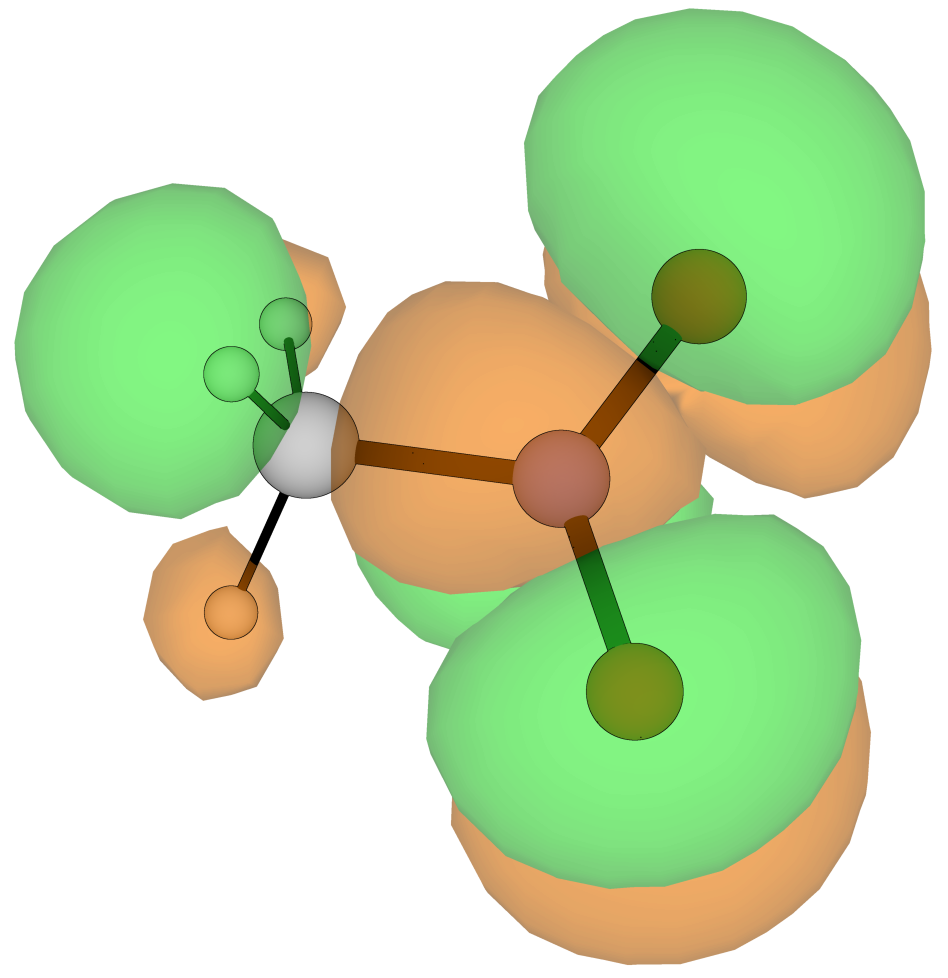
\includegraphics[width=\textwidth]{chapters/introduction/image/MeNO2_VBS.png}
    \small\emph{MeNO\textsubscript{2} VBS anion}
  \end{minipage}
  \hfill
  \begin{minipage}[b]{0.30\textwidth}
    \centering
    \includegraphics[width=\textwidth]{chapters/introduction/image/MeNO2_DBS.png}
    \small\emph{MeNO\textsubscript{2} DBS anion}
  \end{minipage}
  \hfill
  \begin{minipage}[b]{0.3\textwidth}
    \centering
    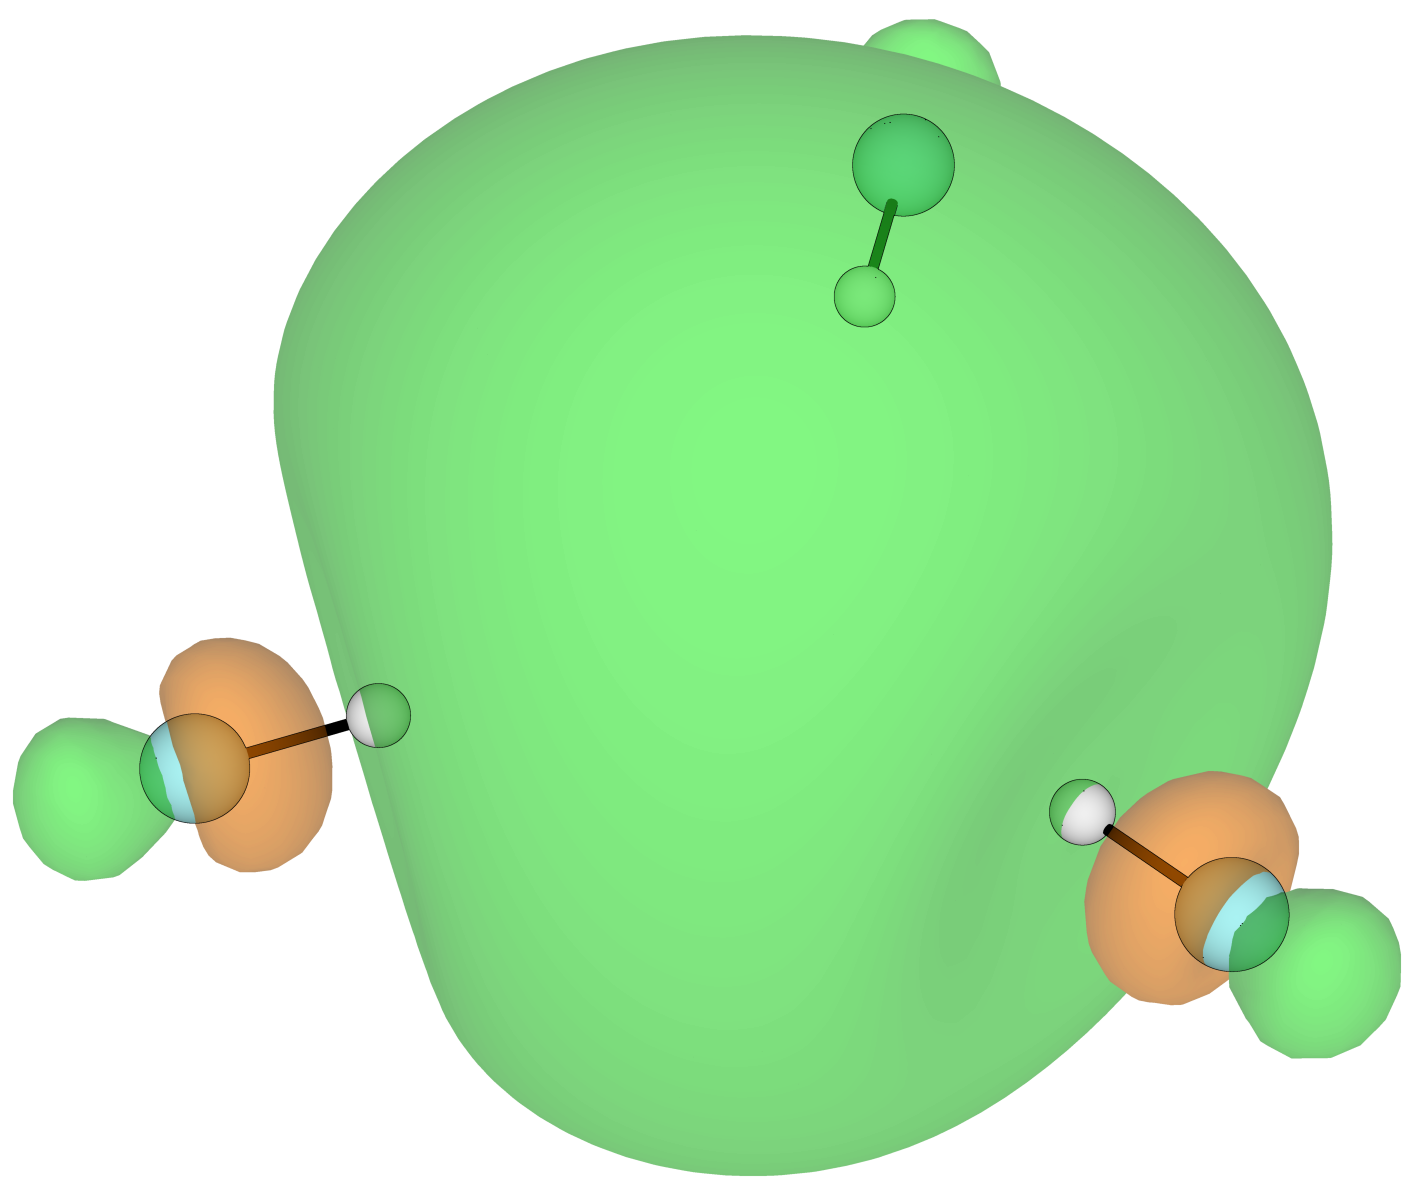
\includegraphics[width=1.1\textwidth]{chapters/introduction/image/hf3.png}
    \small\emph{(HF)\textsubscript{3} solvated electron}
  \end{minipage}
  \caption[Valence and Non-Valence Anions]{Dyson orbital for diferent types of anions computed using EA-EOM-CC2: a) Valence bound state of nitromethane anion, b) dipole bound state of nitromethane, c) solvated electron by a HF trimer. The isosurfaces are set to 0.005 a.u.}
  \label{fig:AnionTypes}
\end{figure}

\subsection{Dipole-Bound Anions}
Of the different non-valence anions, DBSs are the most common and well-studied. They were first proposed in 1947, when it was demonstrated that an ideal dipole could bind an excess electron if the dipole moment exceeds 1.6 D \cite{fermi1947capture}. Further studies regarding `real' molecules, set the now generally accepted critical dipole moment of 2.5 D to bind an extra electron, although having a dipole moment above this threshold does not guarantee the formation of a dipole-bound anion. \cite{jordan2003theory}.

The weak forces that bind the excess electron are responsible for the diffuse nature of the state, with the electronic density often extending several \r{A}ngstr{\"o}ms away from the nuclei, and their relatively low binding energy, usually below 0.1 eV. This makes them susceptible to external perturbations, such as solvent interactions or electric fields, which can significantly influence their stability and reactivity \cite{schiedt1998anion,jalbout2001dipole,gutowski2002solvated,jordan2003theory,eustis2007photoelectron,simons2008molecular,herbert2015quantum,clarke2025role}

DBSs possesses binding energies comparable to thermal energy ($k_bT\,\sim\,23$ meV at room temperature), which might suggest limited practical relevance due to potential detachment. However, DBSs can play a significant role in systems that support both VBSs and NVSs. These systems can undergo a transition from a non-valence anion state to a stable valence state \cite{herbert2015quantum,jordan2003theory}. Moreover, since the electron density of an NVS is spatially extended and resides far from the nuclei, the relaxed structure of an NVS is much closer to that of the neutral molecule compared to a VBS. This large spatial extent also results in a higher cross-section for electron capture and transfer. Consequently, DBSs can act as `doorway' states, facilitating electron capture and transfer processes \cite{hendricks1998dipole,sommerfeld2002coupling,jordan2003theory,sommerfeld2004intramolecular,sommerfeld2005dipole,simons2008molecular,verlet2020role,kang2022state,hassan2022associative,simons2023molecular}. This unique behavior has sparked interest in the role of NVSs across various fields, including astrochemistry \cite{fortenberry2015interstellar} and radiobiology \cite{gu2012interactions,narayanan2023secondary,sedmidubska2024interaction}.

\subsection{Approaches to Study Non-Valence Anions}
Significant progress has been made in experimental and theoretical methods for elucidating the structure and dynamics of NVSs. \cite{desfranccois1995determination,simons2008molecular,simons2023molecular} Experimentally, dipole-bound anions are characterised using spectroscopic techniques designed to probe their weakly bound electronic states \cite{liu2020photoelectron,rogers2019photoelectron,clarke2024dynamics}. In photodetachment and photoelectron spectroscopies, a beam of the target species is generated—often using a laser vaporisation or electrospray source—and probed with light. The energy of the ejected electrons reveals information about the vertical detachment energy and electronic structure of the state. Time-resolved photoelectron spectroscopy (TRPES)\cite{cyr1996femtosecond,neumark2001time} extends this approach, using ultrafast laser pulses to investigate the dynamics of electron attachment and detachment on femtosecond timescales, revealing transient states and relaxation pathways. DBSs can also be accessed by Rydberg electron transfer spectroscopy (RET)\cite{carles2001rydberg,eustis2007photoelectron,bradforth2002excited}, which has been used to probe their role in electron transfer dynamics. Time-of-flight mass spectrometry is often coupled with these techniques to identify and isolate the correct anionic species \cite{desfranccois1996abdoul,ameixa2023parent,pshenichnyuk2020ionizing}.

The theoretical investigation of DBAs presents two main challenges. Firstly, the large spatial extent of the DB orbital requires atomic orbital basis sets that are sufficiently diffuse to accurately describe it, necessitating the use of large custom basis sets \cite{skurski2000choose}. Secondly, electron correlation is important; although the electron density at the valence level remains largely unchanged from the parent molecule, the non-valence part of the density is considerably polarisable due to its diffuse nature and exhibits significant dispersion-like interactions with the valence region, contributing substantially to the binding energy of the extra electron \cite{simons2008molecular,simons2011theoretical,simons2023molecular,gutowski1996contribution,voora2017theoretical}.

Regarding computational methods, standard density functional theory (DFT) approaches can fail because most exchange-correlation functionals cannot properly describe dispersion interactions and can suffer from spin contamination in open-shell molecules \cite{thiam2023accurately}. Multiconfigurational methods like complete active space self-consistent field (CASSCF)\cite{vila2002theoretical,ivanov2015anion} can capture the static correlation of the open shell systems, but require considerable effort in selecting an appropriate active space that balances accuracy and computational feasibility. Moreover, they lack dynamic correlation inherent in the dispersion. Currently, equation-of-motion coupled-cluster (EOM-CC)\cite{herbert2015quantum,jordan2003theory,moorby2024signatures} methods are often used for DBA modelling as they adequately treat both the electron correlation and open-shell character. However, the high computational cost of EOM-CC approaches significantly limits their applicability to small molecular systems. To address this, some approximate methods have been developed, such as the domain-based local pair natural orbital coupled-cluster theory (DLPNO) method\cite{haldar2020multilayer,schulz2018systematic}, or the second order approximate CC2 \cite{christiansen1995second,paran2024performance}, which is used in this work.

\subsection{Non-Valence Anions in Condensed Matter}

Several studies have shown that individual molecules interacting with an NVS-hosting molecule can further stabilise the state by increasing the overall dipole moment or by combining their dipoles to collectively bind the electron within an intermolecular cavity. Moreover, in condensed phase, the excess electron can be stabilised by the interaction of multiple solvent molecules, rather than binding to an individual one, this situation is known as a solvated electron \cite{schiedt1998anion,gutowski2002solvated,jordan2003theory,eustis2007photoelectron,simons2008molecular,herbert2015quantum,clarke2025role}

The binding energy of such solvated electrons can increase dramatically with cluster size. A water molecule does not support any bound anionic state\cite{herbert2015quantum}, however a water dimer anion (H\textsubscript{2}O)\textsubscript{2}\textsuperscript{-} exhibits a low vertical detachment energy (VDE) of 45 meV\cite{coe1990photoelectron}. Water cluster anions (H\textsubscript{2}O)\textsubscript{n}\textsuperscript{-} made of \emph{ca.} 100 molecules can achieve VDEs exceeding 2.0 eV\cite{verlet2005observation}, and in bulk this values is measured to be between 3.4 and 4 eV\cite{coe2008photoelectron,siefermann2010binding}. The structure of the state was the subject of much debate in the literature \cite{kumar2015simple,herbert2019structure,herbert2017hydrated,kevan1981solvated}, but it is now generally accepted that the excess electron resides in a cavity of approximately 2.5 \r{A} in size \cite{herbert2019structure}. This illustrates how solvent molecules can transform a weakly bound non-valence state into a strongly bound electronic species, though with significantly altered properties. 

For solutes, the existence of hydrated NVSs still remains a subject of discussion \cite{anusiewicz2020fate,castellani2019stability,larsen2010does}. Computational studies suggest that hydration influences the localisation of the excess electron, often displacing it onto the surface of the solvent cage \cite{anusiewicz2020fate}. Conversely, experimental evidence indicates that alkyl chains do not disrupt DBS stability \cite{castellani2019stability}, and DBS-mediated mechanisms have been observed in solvated uracil systems \cite{narayanan2024electron}. The viability of NVS in bulk systems depends on the molecular density and polarity of the medium. While solvents may hinder DBS existence due to excluded volume effects, they can also stabilise DBS through Van der Waals interactions \cite{bradforth2002excited,chen2000precursors}. Distinct scenarios can be considered in the interaction between a DBA supporting molecule and solvent: the electron may be found in the NVS orbital, captured by the solvent, or at the interface of the solute and solvent. The latter two phenomena are linked to charge-transfer-to-solvent (CTTS) electronic transitions and are observed experimentally \cite{chen2000precursors,bradforth2002excited,messina2013real,carter2023birth}.

\subsection{Non-Valence Anions in Biological Systems}

Research on dipole-bound anions (DBAs) has predominantly focused on gas-phase systems. However, in biological contexts, DBAs have garnered attention due to their interactions with DNA, particularly in the context of radiation-induced damage and radiosensitizers \cite{gu2012interactions,narayanan2023secondary,sedmidubska2024interaction}.
When high-energy radiation interacts with biological samples, it generates a cascade of secondary electrons which can be captured by cellular constituents, potentially through non-valence states. It has been hypothesised that NVSs in DNA act as electron scavengers, leading to strand breaks and other forms of damage \cite{gu2012interactions,narayanan2023secondary,narayanan2024electron,sommerfeld2005dipole}.
Radiosensitizers are drugs designed to enhance the efficacy of radiation therapy in cancer treatment. These compounds become cytotoxic upon capturing secondary electrons generated during radiation exposure, potentially through the formation of NVSs \cite{sedmidubska2024interaction}.

The role of NVSs in natural biological pathways beyond genetic damage remains largely unexplored, although it has been proposed that vacant pockets in proteins could accommodate non-valence states \cite{castellani2019stability}. Proteins and enzymes play a crucial role in almost all biological reactions, particularly in the transfer and transport of electrons through biological matter. These processes are central to vital phenomena such as photosynthesis \cite{mitchell1961coupling}, aerobic respiration \cite{wikstrom1977proton}, and biological nitrogen fixation \cite{rutledge2020electron}. The range of these electron transfers is remarkable, spanning timescales from picoseconds to milliseconds and distances between donor and final acceptor molecules from a few to over hundreds of \r{A}ngstr{\"o}ms \cite{gray1996electron,blumberger2015recent}. Long-range electron transport is typically achieved through a chain of cofactors, often metal clusters, which facilitate a stepwise transfer of the electron. The inter-cluster distances range from a few \r{A}ngstr{\"o}ms to over 20. As an example, in respiratory complex I, NADH donates electrons to reduce ubquinone\cite{ernster1995biochemical}. The binding sites of both molecules are around 110 \r{A} apart, and the electron transfer is mediated by a series of cofactors. To model these transfer reactions, it is commonly assumed that the electron tunnels between the donor and acceptor. Specifically, in the superexchange model, the tunnelling process is mediated by anionic states in the intervening space, effectively lowering the tunnelling barrier \cite{blumberger2015recent}. The sensitivity of non-valence anion states to environmental factors suggests a potential and elegant mechanism that natural systems could exploit to regulate long-range electron transfer processes. %To the best of my knowledge, no studies have been conducted to investigate this.

This study focuses on other biological targets, which could display an interplay between NVSs and VBSs. A natural compound with relevant roles in electron transfer in biological processes is ubiquinone.

\iffalse DBAs have been used as the explanaiton for the presence of methil functional groups electron of flavins \cite{matthews2018observation}; they would disrupt that state, making the \fi
\begin{figure}[ht!]
  \centering
  \begin{tikzpicture}[x=1pt,y=1pt]
    \node at (137,-11) {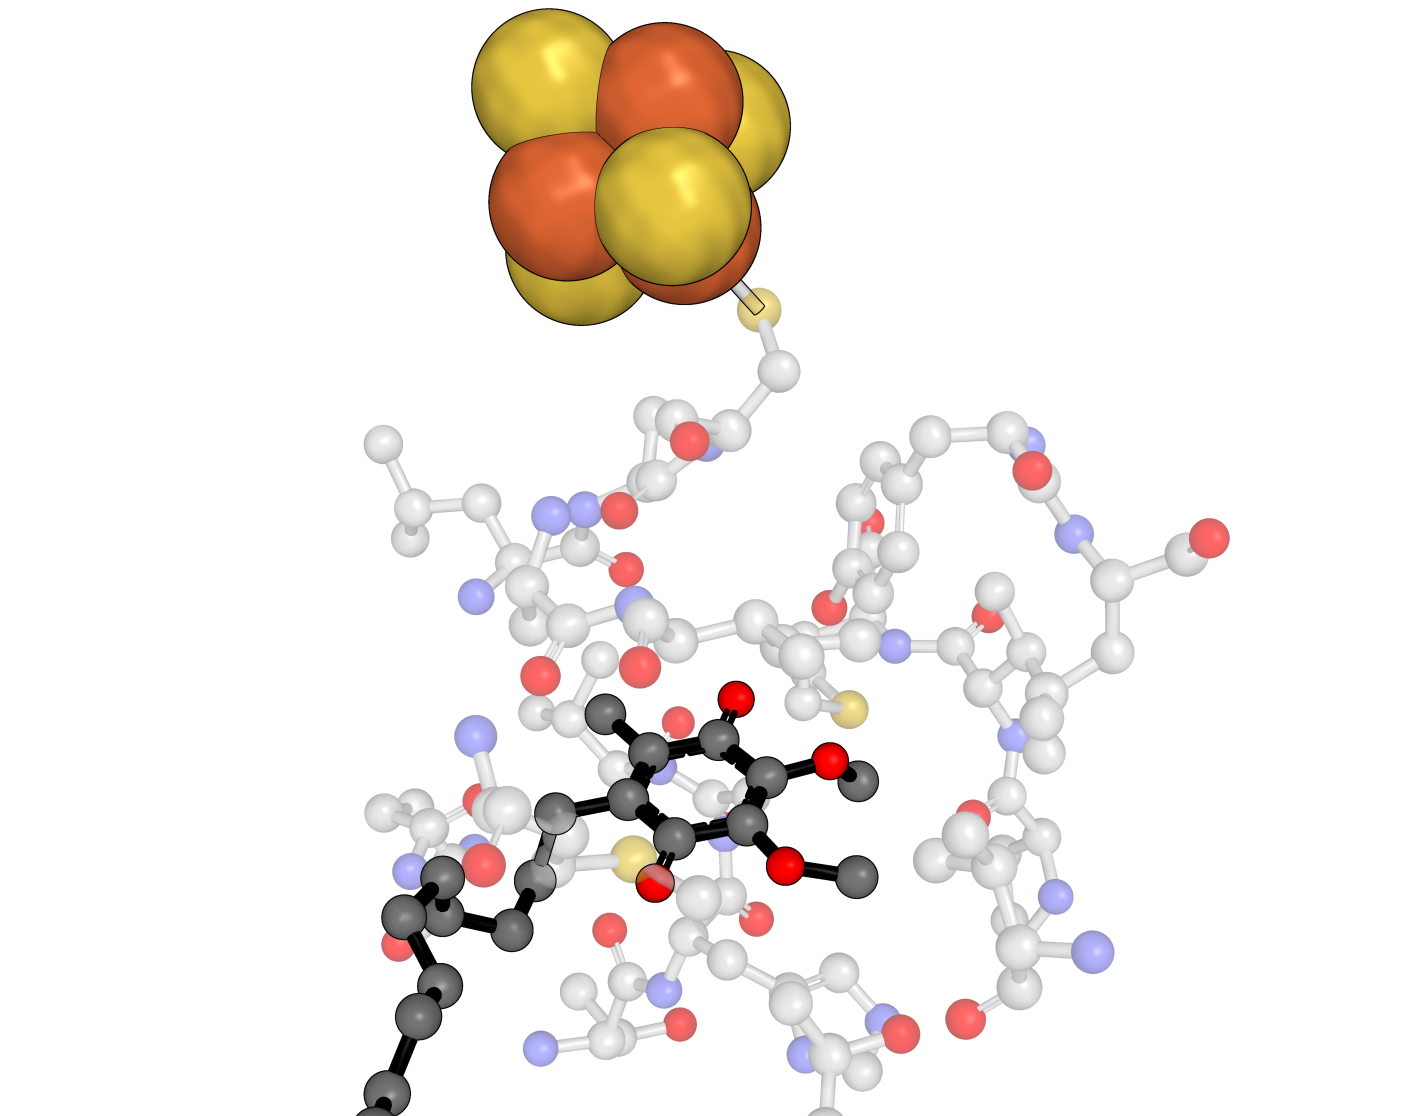
\includegraphics[width=0.45\textwidth]{chapters/introduction/image/uQ_6i0d.png}};
    \node at (205,53) {\includegraphics[width=0.25\textwidth]{chapters/introduction/image/Ubiquinone–ubiquinol_conversion.svg.png}};
    \node at (-50,0) {\includegraphics[width=0.55\textwidth]{chapters/introduction/image/Mitochondrial_electron_transport_chain—Etc4.svg.png}};
  \end{tikzpicture}
  \caption[Role of ubiquinone]{Roles of ubiquinone. Left; electron transport chain in the mitochondria, ubiquinones get reduced at complexes I and II and oxidized at complex III, adapted from Ref. \citenum{ETC2007Wiki}. Right: CoQ at the active site of bacterial complex I (PDB: 6I0D) \cite{gutierrez2020key} and ubiquinone to ubiquinol interconversion.}
  \label{fig:ETC}
\end{figure}

\section{Ubiquinone}
Quinones, named for the bark of the cinchona tree from which they were isolated in the 18th century \cite{rusell1873quinone}, are a class of organic compounds with a fully conjugated cyclic dione structure derived from aromatic compounds by conversion of an even number of C-H to ketone groups \cite{IUPACQ050152025}. Quinones are known for their redox properties and play crucial roles in various biological processes, including electron transport in cellular respiration and photosynthesis \cite{ernster1995biochemical,chen2024low}.

This work focuses on ubiquinone -\textit{ubi} from being ubiquitous in nature-, also known as coenzyme Q (CoQ), a lipid-soluble molecule that can exist as two tautomers: a ketone or alcohol, then named ubiquinol. It plays a role in aerobic respiration in the electron transport chain (ETC) as an electron carrier. As schematised in Figure \ref{fig:ETC}, ubiquinone accepts 2 electrons at complexes I or II and donating them in complex III\cite{ernster1995biochemical}.

Ubiquinone is composed of a benzoquinone ring, 2,3-dimethoxy-6-methyl-p-benzoquinone, and a long side chain, composed of a variable number of isoprenoid units depending on the organism, 10 in humans. This number, \textit{n}, is used for the naming of the specific ubiquinone (Q\textsubscript{n}). In Figure \ref{fig:QuinoneTypes} different Q\textsubscript{n} are presented. The benzoquinone moiety is responsible for its redox properties, while the isoprenoid tail enhances its lipid solubility, allowing it to integrate into biological membranes. \cite{ernster1995biochemical}.

\begin{figure}[ht!]
  \centering
  \begin{tikzpicture}[anchor=south west, x=1cm, y=1cm]
    \node (img1) at (0,20pt) {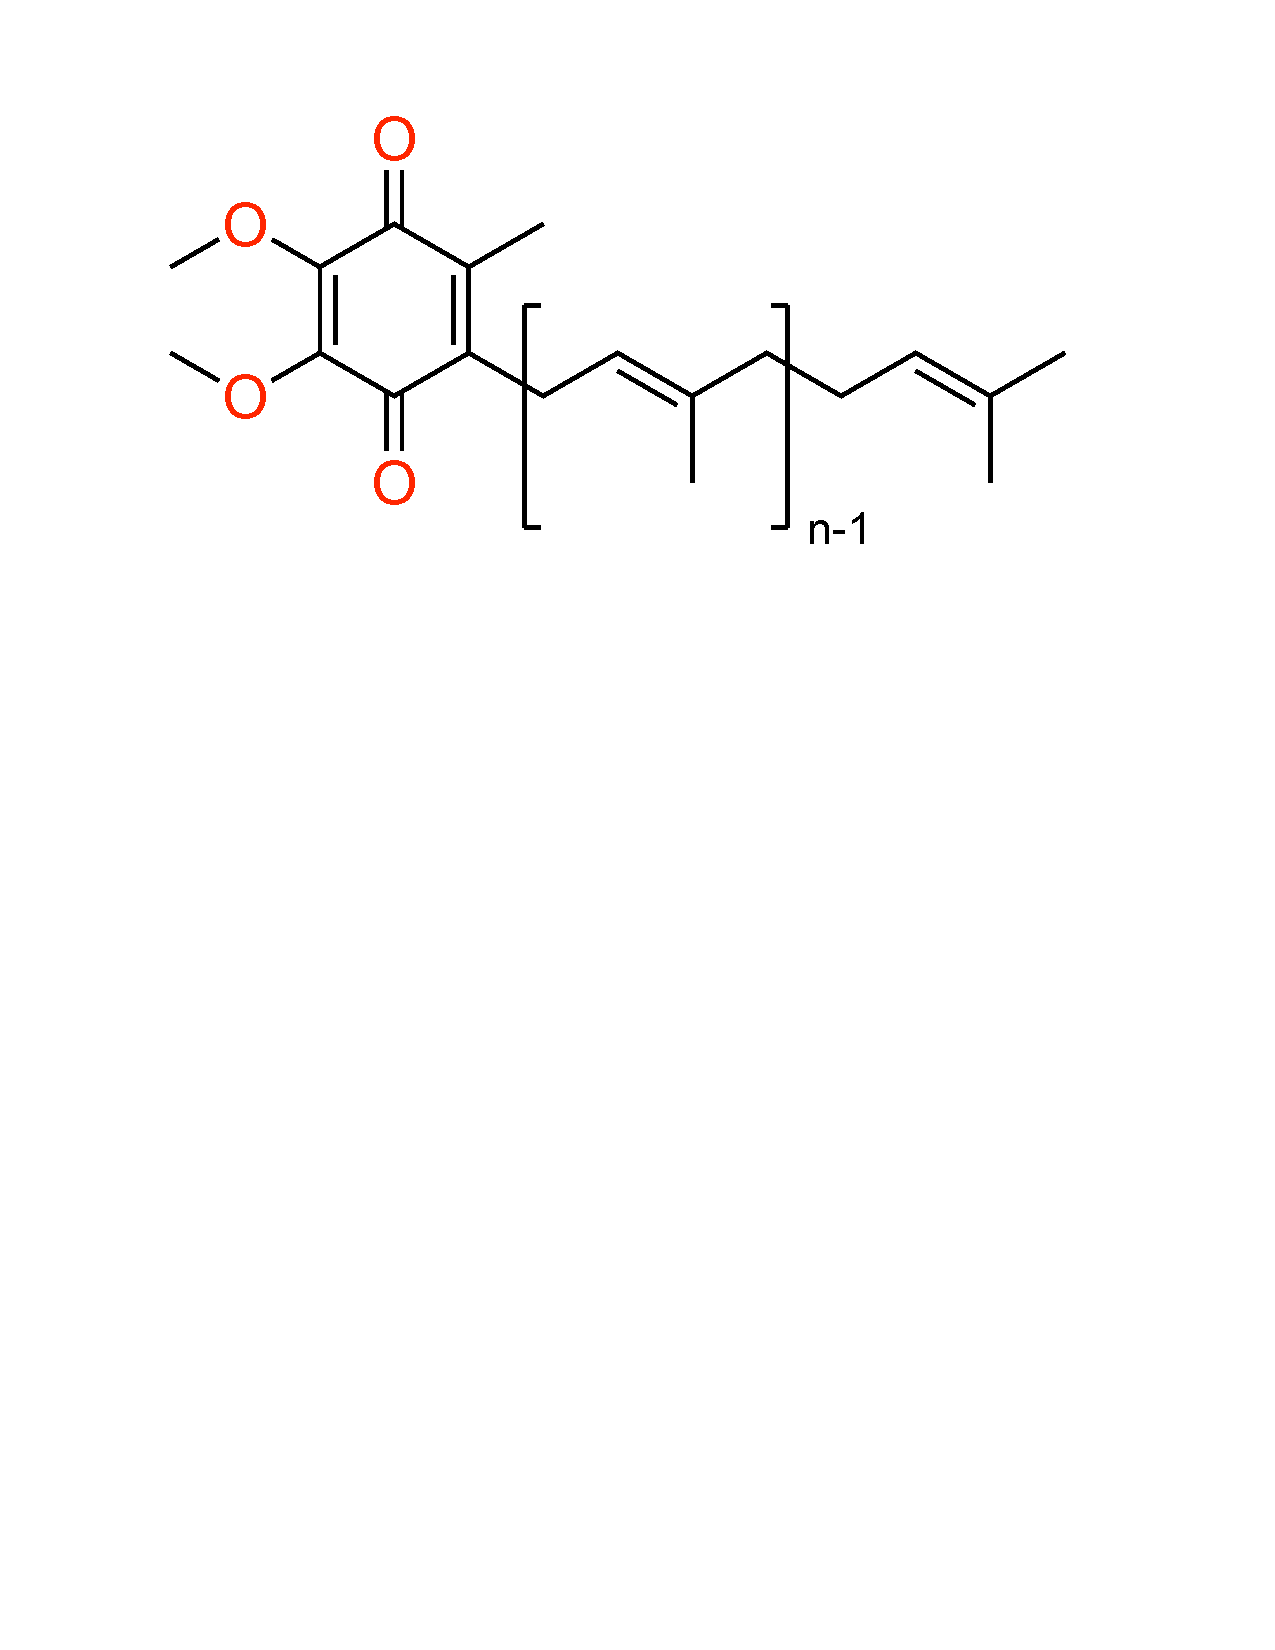
\includegraphics[width=0.45\textwidth]{chapters/introduction/image/UQ_Struct.pdf}};
    \node (img2) at (0.39\textwidth,0) {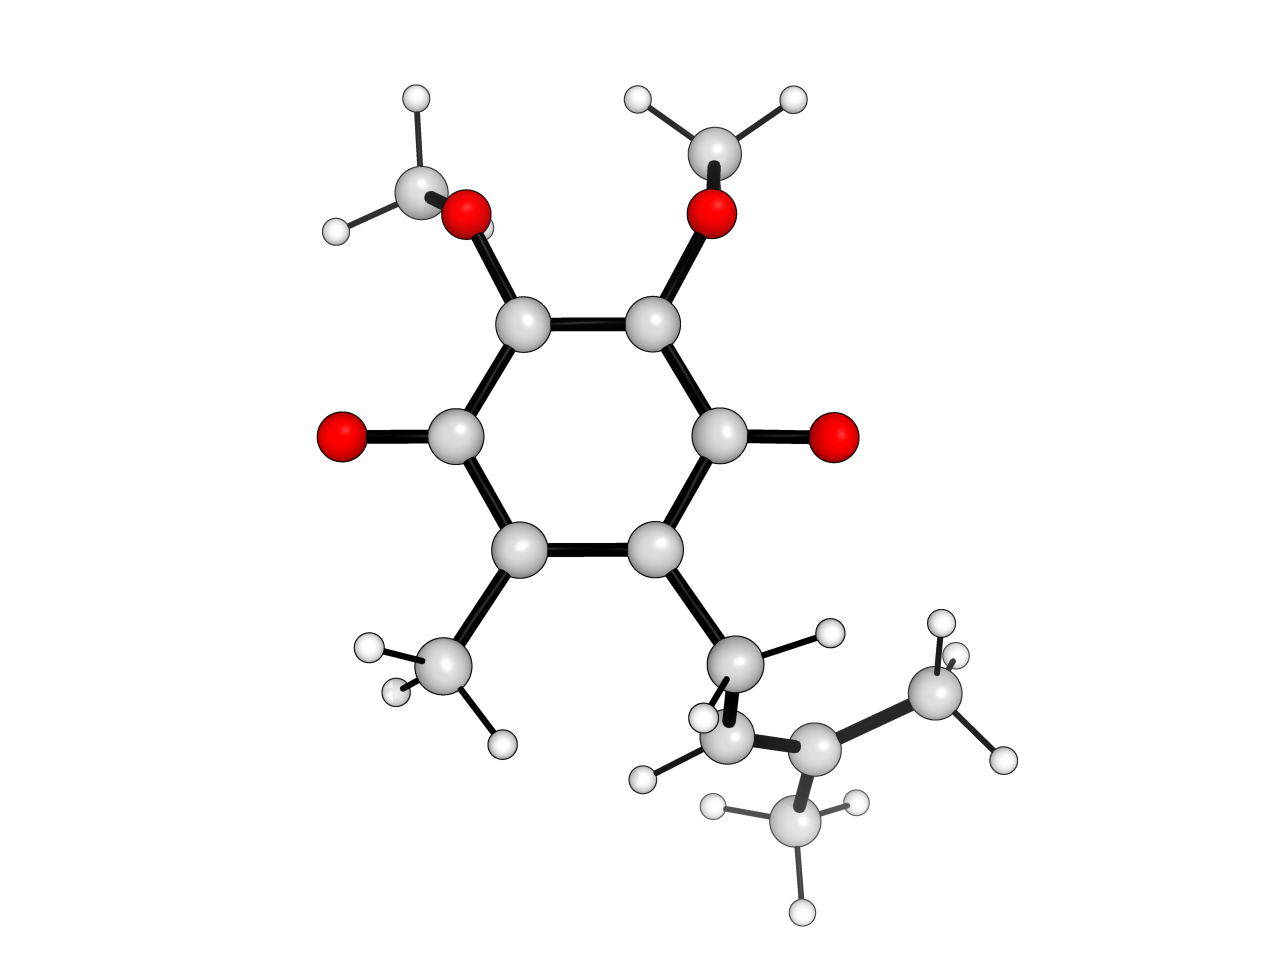
\includegraphics[width=0.4\textwidth]{chapters/introduction/image/Q1.png}};
    \node (img3) at (0.66\textwidth,0) {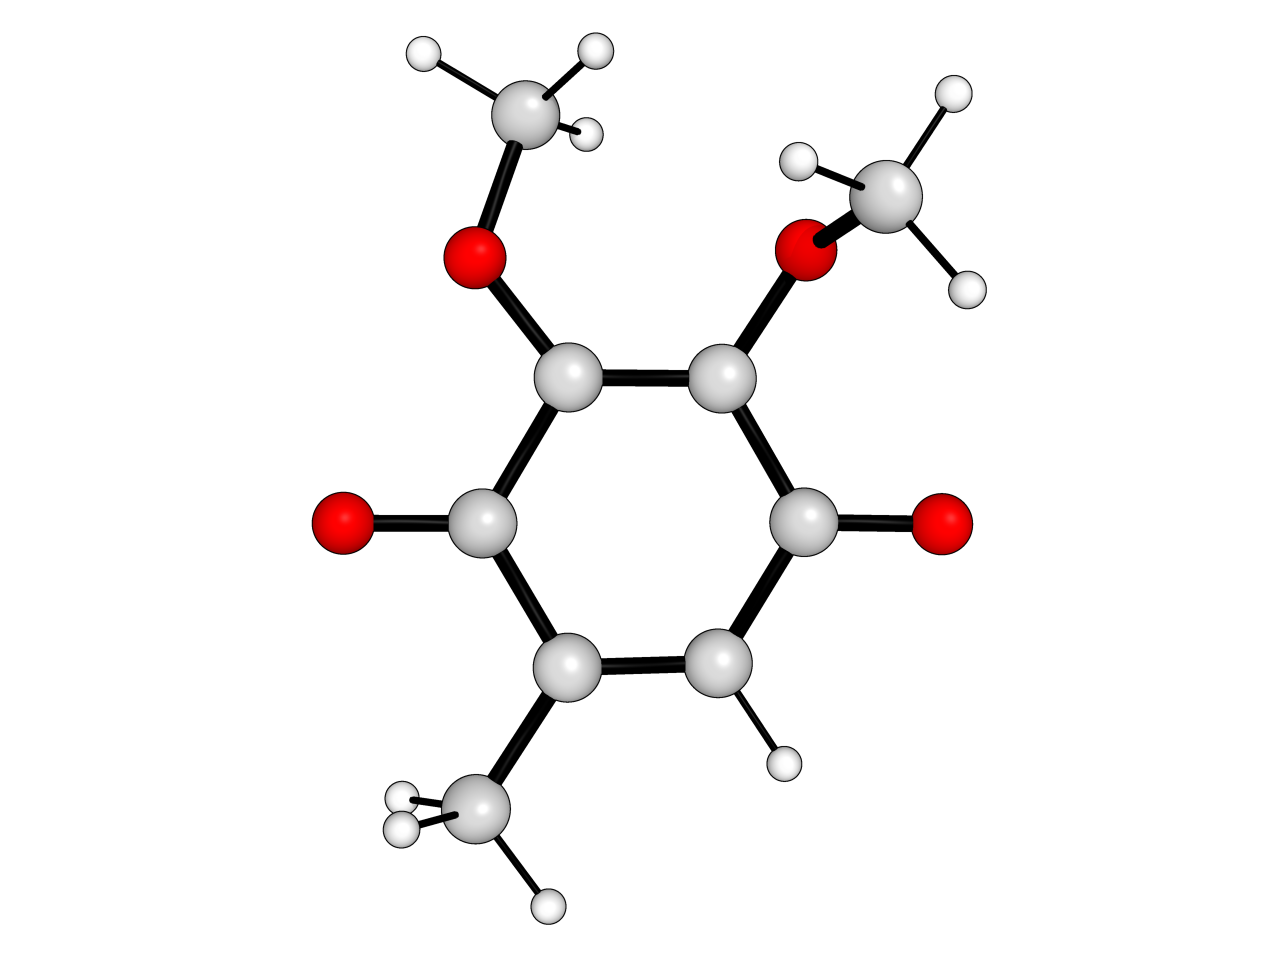
\includegraphics[width=0.4\textwidth]{chapters/introduction/image/Q0189.png}};
    \node[align=center, text=darkgray] at ([yshift=-28pt, xshift=-1.2cm]img1.south) {\footnotesize General structure of CoQ};
    \node[align=center, text=darkgray] at ([yshift=-8pt]img2.south) {\footnotesize Q1};
    \node[align=center, text=darkgray] at ([yshift=-8pt]img3.south) {\footnotesize Q0};
  \end{tikzpicture}
  \caption[Quinone structures]{Quinones considered in this work. From left to right: General structure of CoQ (or Q\textsubscript{n}), Q\textsubscript{1}, Q\textsubscript{0}.}
  \label{fig:QuinoneTypes}
\end{figure}

The ubiquinone moiety can support two types of anion states, a VBS and a DBA. In p-benzoquinone, the valence anion can be understood from the H{\"u}ckel picture with the excess electron occupying a vacant \textpi \textsuperscript{*} orbital. This state is stabilised relative to benzene due to the electron withdrawing ketone groups. In ubiquinone, the VBS is bound by around 1.7 eV \cite{chen2024low}. The dipole-bound anion, on the other hand, results from the two methoxy chains, whose configuration mainly controls the dipole of the molecule \cite{ameixa2023parent}. It is a fairly rigid molecule, except for the dihedral angles between the methoxy groups and the benzoquinone ring and the isoprenoid tail. Their configuration will affect the dipole moment and could therefore determine the existence and energetics of the DBA \cite{ameixa2023parent,bull2015anion}. Therefore, fairly complicated electronic structure can be studied in terms of two coordinates. 

When the isoprenoid tail is considered, it has been shown that it further stabilises the valence anion \cite{pshenichnyuk2020ionizing}. Its effects on the dipole state have not been studied. One can imagine the effect to be moderate for shorter tails; it will slightly modify the dipole moment of the system, but structurally will be quite far from the excess electron density. For longer tails, the isoprenoid chain could sterically hinder the dipole-bound state.

There have been extensive studies on the electron binding properties of the ubiquinone family, both experimentally \cite{ameixa2023parent,west2014anion,pshenichnyuk2020ionizing,bull2015anion} and theoretically \cite{ameixa2023parent,pshenichnyuk2020ionizing,haldar2020multilayer, nonella1998quantum, gamiz2017terminal}. However, these studies have focused on the valence anion of the quinone, and no comprehensive study of the dipole bound state has been performed. The VBS is the final acceptor of the electron and the existence of the DBA in condensed phase is dubious.
However, experimental studies have observed dipole-bound anions in the gas phase in ubiquinones Q\textsubscript{0} and Q\textsubscript{1}\cite{ameixa2023parent}. Although its signal is reduced as more isoprenoid units are added, interpreted as an effect of the isprenoid tail being flexible and resulting in a steric hindrance of the state \cite{ameixa2023parent,pshenichnyuk2020ionizing}, one could imagine that in a protein moiety, the geometry of the tail would be fixed far from a potential DB orbital, which could even be further stabilised by residues pointing in the cavity. This motivates the current study.

\section{Research Goals}
The main objective of this work is to theoretically study the dipole-bound anions of ubiquinone. The electron attachment variant of equation-of-motion CC2 (EA-EOM-CC2) is used, which has recently shown to be adequate for dipole bound states of organic molecules \cite{paran2024performance}. The specific objectives are:
\begin{itemize}
  \item Benchmark the reliability of the EA-EOM-CC2 method to compute the electron affinity of quinones.
  \item Implement the Dyson orbital approach for EOM-CC2, for characterisation of electronic states of large systems beyond their energies.
  \item To investigate the dipole-bound anions of ubiquinone in terms of its functional group configurations.
  \item To study the effect of the molecular environment on the dipole-bound anion of ubiquinone.
\end{itemize}

%%%%%%%%%%%%%%%%%%%%%%%%%%%%%%%%%%%%%%%%%%%%%%%%%%
% Keep the following \cleardoublepage at the end of this file, 
% otherwise \includeonly includes empty pages.
\cleardoublepage

% vim: tw=70 nocindent expandtab foldmethod=marker foldmarker={{{}{,}{}}}

% !TeX root = ../../thesis.tex
\chapter{Theoretical Background}\label{ch:theory}

\section{Self Consistent Field Methods} \label{sec:SCF}
The Hartree-Fock (HF) method stands as a method in electronic structure theory. Its primary objective is to provide an approximate solution to the many-electron time-independent Schrödinger equation within the Born-Openhaimer approximation, which governs the behavior of electrons within atoms and molecules:
\begin{equation}\label{eq:TISE}
    \hat{H}_e \Psi_e = E_e \Psi_e
\end{equation}
The HF method achieves this by assuming that each electron moves independently within an average electrostatic field generated by all the other electrons in the system. In the HF method the \textit{N}-electron wavefunctionis is represented by a Slater determinant, which is formed by taking the antisymmetrized product of N individual one-electron wavefunctions, the spin-orbitals ($\chi$):
\begin{equation}\label{eq:SlaterDet}
    \Psi(\mathbf{r}_1, \mathbf{r}_2, \dots, \mathbf{r}_N) = \frac{1}{\sqrt{N!}}
    \begin{vmatrix}
      \chi_1(\mathbf{r}_1) & \chi_2(\mathbf{r}_1) & \cdots & \chi_N(\mathbf{r}_1) \\
      \chi_1(\mathbf{r}_2) & \chi_2(\mathbf{r}_2) & \cdots & \chi_N(\mathbf{r}_2) \\
      \vdots & \vdots & \ddots & \vdots \\
      \chi_1(\mathbf{r}_N) & \chi_2(\mathbf{r}_N) & \cdots & \chi_N(\mathbf{r}_N)
    \end{vmatrix}
  \end{equation}
The determinantal inherently satisfies both the Pauli exclusion principle, and the antisymmetry requirement of fermions. The energy expectation for a Slater determinant according to HF is variational and can be computed as:
\begin{equation}\label{EHF}
    \begin{aligned}
        E_{HF} &= \sum_{i=1}^{N} \hat{F}_i \Psi \\
            &= \sum_{i=1}^{N} \hat{h}(i) + \sum_{i,j=1}^{N} (\hat{J}_j(i) - \hat{K}_j(i)) \\ 
            &= \sum_{i=1}^{N} \langle \chi_i | \hat{h} | \chi_i \rangle + \frac{1}{2} \sum_{i,j=1}^{N} \langle \chi_i \chi_j || \chi_i \chi_j \rangle
    \end{aligned}
\end{equation}
Where, $\hat{F}$ is the Fock operator. $\hat{F}$ is made up from $\hat{h}$, the one-electron core Hamiltonian operator (kinetic energy and electron-nucleus attraction); $\hat{J}_j(i)$, the Coulomb operator, describing the electrostatic repulsion between electron i and the average charge distribution of electron j, and $\hat{K}_j(i)$ is the exchange operator, a purely quantum mechanical term arising from the antisymmetry principle. \\
The Hartree-Fock equations are inherently non-linear because the Fock operator depends on the wavefunctions of all the other electrons, their interactions are coupled. Consequently, these equations cannot be solved analitically and necessitate an iterative procedure known as the Self-Consistent Field (SCF) method.

\subsection{Electron Correlation}
\label{subsec:electron_correlation}
The Hartree-Fock (HF) method is inherently limited by its neglect of the instantaneous correlation between the motions of electrons. In the HF approximation, each electron is treated as moving independently within a static, average field created by all other electrons. This mean-field approach fails to account for the fact that electrons, being negatively charged, will instantaneously repel each other, leading to a dynamic correlation in their movements as they try to avoid each other in space.\\
This neglection leads to an overestimation of the electron-electron repulsion energy, and is responsible for its inability to accurately predict certain phenomena, such as London dispersion forces. The difference between the exact non-relativistic energy of the system and the energy obtained in the Hartree-Fock limit is defined as the correlation energy and is always negative due to the variational principle. Correlated methods aim to include the effects of the instantaneous interactions between electrons that are neglected in the mean-field approximation of HF theory. Several correlated methods used during this work are:

\subsection{Møller-Plesset Perturbation Theory}
Møller-Plesset (MP) perturbation theory offers a systematic way to improve upon the HF energy by treating the electron correlation as a perturbation to the Hartree-Fock Hamiltonian.The Fock operator is taken as the zeroth-order Hamiltonian, and the difference between the exact electron-electron repulsion and the Fock operator is considered the perturbation. The energy and wavefunction are then expanded as a series in terms of the perturbation strength. The first-order energy correction in MP theory is zero, so the first non-trivial correction to the HF energy appears at the second order, giving rise to the MP2 method. The MP2 energy correction for a closed-shell molecule is given by:
\begin{equation} \label{eq:MP2}
    E_{MP2} = - \frac{1}{4} \sum_{ij}^{occ} \sum_{ab}^{virt} \frac{|\langle i j || a b \rangle|^2}{\epsilon_a + \epsilon_b - \epsilon_i - \epsilon_j}
\end{equation}
Where $i,j$ denote occupied molecular orbitals, $a,b$ denote virtual molecular orbitals, and $\epsilon$ are the corresponding orbital energies from the HF calculation. MP theory can be extended to higher orders (MP3, MP4, etc.) to achieve greater accuracy, although the computational cost increases significantly with each order.

\subsection{Density Functional Theory}
Density Functional Theory (DFT) provides an alternative approach to incorporating electron correlation by focusing on the electron density of the system rather than the wavefunction, reducing the degrees of freedom of the system from $3N-3$ to just $3$. The fundamental principle of DFT is that the ground state energy of a system is a unique functional of its electron density:
\begin{equation}\label{eq:KSDFT}
    \left( -\frac{1}{2} \nabla^2 + V_{ext}(\mathbf{r}) + V_H(\mathbf{r}) + V_{XC}[\rho(\mathbf{r})] \right) \psi_i(\mathbf{r}) = \epsilon_i \psi_i(\mathbf{r})
\end{equation}
Where $V_ext$ respresents the external potential, $V_H(\mathbf{r}) = \int \frac{\rho(\mathbf{r}')}{|\mathbf{r} - \mathbf{r}'|} d\mathbf{r}'$ is the hartree potential, $V_{XC}$ is the Exchange-Correlation potential and $\rho(\mathbf{r})$ is the electron density. The exchange-correlation functional is the most challenging part of DFT, as it is not known exactly and must be approximated. The accuracy of DFT calculations depends heavily on the choice of exchange-correlation functional.

\subsection{Configuration Interaction}
Configuration Interaction (CI) methods improve upon HF by expressing the electronic wavefunction as a linear combination of the HF ground state determinant and excited state determinants:
\begin{equation} \label{eq:CI}
     |\Psi_{CI} \rangle = c_0 |\Phi_0 \rangle + \sum_{ia} c_{ia} |\Phi_{ia} \rangle + \sum_{ijab} c_{ijab} |\Phi_{ijab} \rangle + \dots
\end{equation}
Where $|\Phi_0 \rangle$ is the HF ground state determinant, $|\Phi_{ia} \rangle$ represents a wavefunction with a hole in spin-orbital \textit{i} and a particle in the spin-orbital \textit{a}, and c are the CI coefficients. Full CI, which includes all possible excited determinants, is exact within the basis set but computationally prohibitive for all but the simplest systems. Truncated CI methods, such as CIS (singles) and CISD (singles and doubles), are more practical but lack size extensivity.

\subsection{Coupled Cluster Theory} \label{sec:CCTheory}
The coupled cluster (CC) theory is considered the gold-standard method in quantum chemistry. Similarly to CI, the CC method expands the wavefunction as a liinear combination of Slater determinats. However, the CC method results into a size-extensive and size-consistent wavefunction by using an exponential ansatz.
\begin{equation}\label{CCWavefunc}
    | \Psi_{CC} \rangle = e^{\hat{T}} | \Psi_{0} \rangle
\end{equation}
\\Where $\hat{T}$ is the cluster operator, which is the central component of CC theory and is defined as a sum of excitation operators:
\begin{equation}
    \hat{T} = \hat{T}_1 + \hat{T}_2 + \hat{T}_3 + \dots + \hat{T}_N
\end{equation}
where $N$ is the total number of electrons in the system. Each term in this sum corresponds to a specific level of excitation:
\begin{itemize}
    \item $\hat{T}_1 = \sum_{i}^{\text{occ}} \sum_{a}^{\text{virt}} t_i^a a_a^{\dagger} a_i$ represents single excitations.
    \item $\hat{T}_2 = \frac{1}{4} \sum_{i,j}^{\text{occ}} \sum_{a,b}^{\text{virt}} t_{ij}^{ab} a_a^{\dagger} a_b^{\dagger} a_j a_i$ represents double excitations.
    \item Higher-order excitation operators $\hat{T}_3, \hat{T}_4, \dots$ describe simultaneous excitation of three, four, and more electrons.
\end{itemize}
The coefficients $t_i^a$, $t_{ij}^{ab}$, etc., are cluster amplitudes to determined by solving the coupled cluster Schr\"{o}dinger equation. The energy of the system is obtained by projecting the Schrödinger equation onto the Hartree-Fock reference determinant:
\iffalse One of the most significant advantages of coupled cluster theory is its property of size consistency. A size-consistent method correctly describes the energy of a system composed of multiple non-interacting subsystems as the sum of the energies of the individual subsystems. The exponential form, when expanded as a Taylor series,
\begin{equation}
    e^{\hat{T}} = 1 + \hat{T} + \frac{1}{2!} \hat{T}^2 + \dots
\end{equation}
inherently includes terms that represent disconnected clusters, which are essential for size consistency. \fi
\begin{equation}\label{eq:CCEnergy}
    E_{CC}=\langle \Psi_{0} | e^{-\hat{T}} \hat{H} e^{\hat{T}} | \Psi_{0} \rangle
\end{equation}
Using the Baker-Campbell-Hausdorff (BCH) expansion, the exponential operators in Eq. \ref{eq:CCEnergy} can be simplified to a series of commutators which ends at the fourth order. The cluster operator $\hat{T}$ can be truncated at different levels of excitation:
\begin{itemize}
    \item \textbf{CCD} (Coupled Cluster Doubles): This is the simplest approximation in the CC family, where the cluster operator is truncated to include only single excitations: $\hat{T} \approx \hat{T}_2$. Due to the Brilluin's theorem, the amplitudes of single excitations are 0. 
    \item \textbf{CCSD} (Coupled Cluster Singles and Doubles): This is one of the most widely used and generally accurate coupled cluster methods, where the cluster operator includes both single and double excitations:$\hat{T} \approx \hat{T}_1 + \hat{T}_2$.
    \item \textbf{CCSDT} (Coupled Cluster Singles, Doubles, and Triples): $\hat{T} \approx \hat{T}_1 + \hat{T}_2 + \hat{T}_3$.
    The hierarchy can be extended to include even higher levels of excitation, converging to the Full Configuration Interaction (Full CI) limit. Full CI includes all possible excitations within a given one-electron basis set and represents the exact solution to the non-relativistic Schrödinger equation in that basis.
\end{itemize}
\begin{table}[h!]
    \centering
    \begin{tabular}{ccc}
        Method & Operation count & Memory \\
        \hline
        HF & $O(N^4)$ & $O(N^4)$ \\
        MP2 & $O(N^5)$ & $O(N^4)$ \\
        CCD/CCSD & $O(N^6)$ & $O(N^4)$ \\
        CCSDT & $O(N^8)$ & $O(N^6)$ \\
        CC2 & $O(N^{5})$ & $O(N^4)$ \\
    \end{tabular}
    \caption{Computational scaling of quantum chemistry methods.}
    \label{tab:qc_scaling}
\end{table}

\subsection{Second Approximate Coupled Cluster}\label{sec:CC2Theory}
Second Approximate Coupled Cluster (CC2) belongs to the broader family of CCn approximate coupled cluster methods, where the 'n' in CCn indicates the level of approximation within a perturbative hierarchy. These methods aim to reduce the computational cost associated with standard CC truncations while still retaining a reasonable level of accuracy.\\

In CC2 the equations for the single amplitudes ($t^a_i$) are the same as those in CCSD, while the doubles amplitudes ($t^ab_ij$) are calculated using the non-iterative expression for MP2 (Eq \ref{eq:MP2}). The resulting expression for the CC2 correlation energy is:
\begin{equation}\label{CC2Energy}
    E_{CC2} = \sum_{ij}^{occ} \sum_{ab}^{virt} \frac{1}{4}\frac{|\langle i j || a b \rangle|^2}{\epsilon_a + \epsilon_b - \epsilon_i - \epsilon_j}  + \sum_{i}^{occ} \sum_{a}^{virt} \hat{F}_{ai} t^a_i 
\end{equation}

The perturbative treatment of the doubles amplitudes in CC2, reduces the computational cost compared to CCSD, Table \ref{tab:qc_scaling}. While this approximation can lead to a less accurate description of electron correlation, the inclusion of zeroth-order singles amplitudes allows for an approximate description of orbital relaxation, which often leads to higher quality results compared to MP2.

\section{Equation-of-Motion Methods} \label{sec:eom_theory}
Equation-of-Motion Coupled Cluster (EOM-CC) methods are an extension of ground-state coupled cluster theory which provide a framework for calculating a variety of excited (EE), ionized (IP) and electron-attached (EA) states. In the EOM-CC, the target electronic state is described by applying a linear excitation operator $\hat{R}$ to a reference state, which typically is the coupled cluster wavefunction of the ground state. The target state wavefunction can then be expressed as $|\Psi_{\text{EOM}}\rangle = \hat{R} |\Psi_{\text{CC}}\rangle = \hat{R} e^{\hat{T}} |\Phi_{\text{HF}}\rangle$.\\
The form of the operator $\hat{R}$ is similar to the cluster operator and chosen to access the desired target state. In the case of EOM-EA, the electron attachment operator $R_{EA}$ includes terms that describe the addition of one electron to an unoccupied orbital (a one-particle creation operator), terms that describe the addition of one electron accompanied by the excitation of another electron from an occupied to an unoccupied orbital (a two-particle and one-hole creation operator), and so on:
\begin{equation}\label{eq:R_EA}
    \hat{R}_{EA} = \hat{R}_{1_{EA}} + \hat{R}_{2_{EA}} + \ldots = \sum_{a} r^a a_a^{\dagger} + \frac{1}{2}\sum_{ab} \sum_{i} r^{ba}_{i} a_b^{\dagger} a_a^{\dagger} a_i + \ldots
\end{equation}
\begin{figure}
    \centering
    \medskip
    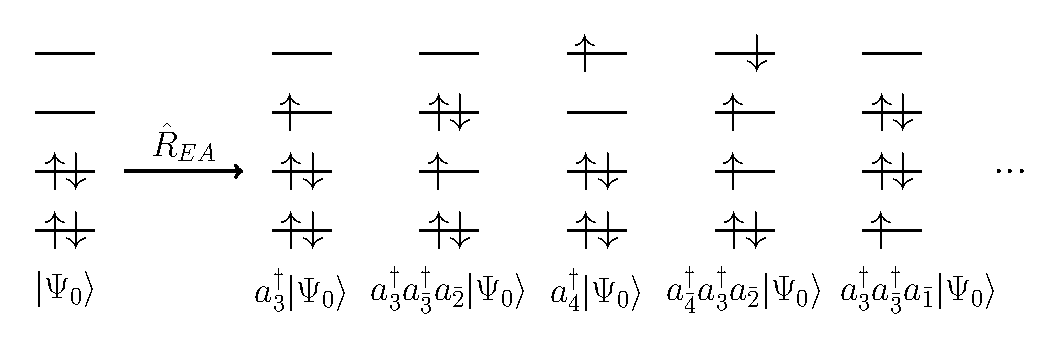
\includegraphics[width=.7\textwidth]{EOM_EA}
    \caption{EOM-EA.}
    \label{fig:EOM}
  \end{figure}

  Where $a$ and $b$ denote virtual orbitals, $i$ denotes an occupied orbital, and $r^a$ and $r^{ba}_{i}$ are the coefficients (amplitudes) to be determined. The electron affinities (EAs) of the system are then obtained as the eigenvalues of the similarity-transformed Hamiltonian:
\begin{equation}
    \bar{H}_{N} \bar{R} | \Psi_0 \rangle = \Delta E_{EOM} \bar{R} | \Psi_0 \rangle
\end{equation}
\begin{equation}
    \bar{H}_{N} = e^{-T} H e^{T} - \langle \Psi_0 | e^{-T} H e^{T} | \Psi_0 \rangle
\end{equation}

\subsection{Dyson orbitals}

Dyson orbitals are defined as the overlap between the wavefunction of an initial $N$-electron state ($|\Psi_0^N\rangle$) and the wavefunction of the final state with $N\pm1$ electrons ($|\Psi_f^{N\pm1}\rangle$).
\begin{equation}\label{eq:dyson}
    \phi_{d} = \langle \Psi_0^N | \Psi_f^{N\pm1} \rangle = \langle \Psi_0^N | \hat{R}\,\Psi_0^{N} \rangle 
\end{equation}

Because the the terms differ in one electron, the result of the overlap is a vector instead of a scalar, and can be expressed as a linear combination of the molecular orbitals ($\phi_p(r)$) of the reference wavefunction:

\begin{equation}
    \phi_{Dyson}(r) = \sum_p \gamma_p \phi_p(r)
\end{equation}

where $\gamma_p$ are the coefficients that quantify the contribution of each molecular orbital to the Dyson orbital.\\

Physically, Dyson orbitals can be interpreted as representing the correlated state of the electron that is either removed or added to it. They can be used for the interpretation and prediction of photoelectron spectra as they contain all the information required to calculate diffrential corss-sections, $\frac{d\sigma}{d\Omega_k}$:

\begin{equation}
    \frac{d\sigma}{d\Omega_k} = \frac{4\pi^2kE}{c}|\langle \phi_d | \mu | \Psi^{el}_k \rangle |^2
\end{equation}

Where where \textit{k} is the magnitude of the photoelectron wavevector, \textit{E} is the energy of the ionizing radiation, and \textit{c} is the speed of light, $\mu$ is the dipole operator, and $\Psi^{el}_k$ is the photoelectron wavefunction. 

%%%%%%%%%%%%%%%%%%%%%%%%%%%%%%%%%%%%%%%%%%%%%%%%%%
% Keep the following \cleardoublepage at the end of this file, 
% otherwise \includeonly includes empty pages.
\cleardoublepage

% vim: tw=70 nocindent expandtab foldmethod=marker foldmarker={{{}{,}{}}}
% !TeX root = ../../thesis.tex
\chapter{Computational Methods}\label{ch:methods}

All electronic structure calculations were performed using the developer's copy of the \textit{QChem} software \cite{QChem5}. In all computations the frozen-core
approximation is used, only the valence orbitals are correlated, as well as the resolution of the identity (RI) approximation, auxiliary basis functions are used to approximate the Coulumb operator integrals, reducing its scaling to $N(O^3)$ \cite{hattig2000cc2}.

For the EOM-EA calculations, the reference wavefunction was obtained as the restricted Hartree-Fock (RHF) solution of the ground state of the neutral molecule. Unless explecitly mention, calculations were performed at using the aug-cc-pVDZ basis set \cite{dunning1989gaussian} further augmented by 3 s-shells on hydrogen atoms and 6 s- and 3 p-shells on all non-hydrogen atoms \cite{paran2024performance} to properly model the non-valence states. The coefficients of the extra functions were obtained by halving the most diffuse function of the original set.

Photoionization and Photodetachment crossections were calculated using the \textit{ezDyson} package \cite{gozem2022ezspectra,gozem2015photoionization}.






%%%%%%%%%%%%%%%%%%%%%%%%%%%%%%%%%%%%%%%%%%%%%%%%%%
% Keep the following \cleardoublepage at the end of this file, 
% otherwise \includeonly includes empty pages.
\cleardoublepage


% vim: tw=70 nocindent expandtab foldmethod=marker foldmarker={{{}{,}{}}}
% !TeX root = ../../thesis.tex
\chapter{Results and Discussion}

\section{Performance of EOM-CC2 Methods}
This section examines the performance of the EA-EOM-CC2 method for calculating electron affinities. Previous work has shown that EA-EOM-CC2 performs adequately for dipole-bound states (DBSs), whilst tending to overestimate vertical electron affinities (VEAs) for valence-bound states (VBSs) \cite{paran2024performance}. The following analysis focuses on three aspects: the basis set dependence for DBSs in section \ref{sec:results:basis}, the method's performance for VBSs using a test set of quinones in section \ref{sec:results:quinones}, and the efficacy of CC2 in generating Dyson orbitals through comparison of photodetachment cross-sections calculated with EOM-CC2, EOM-CCSD and HF in section \ref{sec:results:crosssection}.

\subsection{Basis Set Dependence of EA-EOM-CC2 in Dipole Bound Anions} \label{sec:results:basis}

The basis set dependence of EA-EOM-CC2 for dipole-bound radical anions was evaluated using a test set of 14 DBS of organic molecules taking as reference EA-EOM-CCSD \cite{paran2024performance}. The results as summarised in Table \ref{tab:basis}. The binding energies range from less than 1 meV for acetone to approximately 26 meV for nitrobenzene. The table also shows how the binding energy does not correlate strongly with the magnitude of the dipole moment for different species. For instance, phenylisocyanide, which has a slightly lower dipole moment than benzaldehyde, exhibits an electron affinity nearly twice as large.\\

The basis set cardinality was varied from DZ to QZ for EA-EOM-CC2 and from DZ to TZ for CCSD, while keeping additional diffuse functions fixed at 6s3p, \textit{vide infra}, for heavy atoms and 3s for hydrogens, referred to as (6s3p). For the EA-EOM-CC2 method, the influence of diffuse functions was further explored by fixing the cardinality to TZ and incrementally increasing the number of diffuse functions from 2s1p for heavy atoms and 1s for hydrogens, referred to as (2s1p), to 8s4p for heavy atoms and 4s for hydrogens, referred to as (8s4p). The exponents of the diffuse functions are detailed in the methods' section \ref{sec:methods:basis}. For comparison, the dipole strength, calculated at the HF level, and Koopmans' theorem (KT), which estimates the binding energy using the energy of the lowest unoccupied molecular orbital, are also included.\\

Starting with the simplest approximation, KT predicts that all anions with an EOM-EA-CCSD binding energy below 10 meV are unbound. However, even for more strongly bound cases, Koopmans' theorem significantly underestimates the binding energy, capturing only 20\% of the binding energy for nitrobenzene, for example.\\

No DBS is found when only the 2s1p diffuse function are added. At the 6s3p level the DBS energy is converged with respect to the extra diffuse functions added to the basis set, deviating by less than 1 meV from the value obtained with the 8s4p diffuse function. The errors are more pronounced for smaller molecules, such as acetaldehyde and acetone. This could be attributed to the inability of functions centred on a few atoms to adequately cover the spatial extent of the DBS orbital. This reasoning may also explain why the DBS of acetaldehyde is only predicted by RI-EA-EOM-CC2/aug-cc-pVTZ+8s4p, as it employs the most diffuse functions. At the RI-EA-EOM-CCSD/aug-cc-pVTZ+8s4p, the DBS of acetaldehyde is found to be 0.84 meV, compared to the 0.76 meV of CC2.\\

The binding energy increases with higher cardinality, as expected, due to the increased flexibility of the basis set. However, this effect is less significant than the addition of diffuse functions. For instance, the difference between RI-EA-EOM-CCSD/aug-cc-pVDZ+6s3p and RI-EA-EOM-CCSD/aug-cc-pVTZ+6s3p is less than 1 meV for most cases. Smaller molecules with lower-energy DBSs tend to be more challenging; for example, a TZ basis is required to predict the DBS of acetone. In general, and especially for larger systems, the inclusion of diffuse functions is more critical than the cardinality of the basis set for dipole-bound anions.\\

CC2/aug-cc-pVTZ+6s3p consistently overestimates the binding energies across all molecules when compared to CCSD/aug-cc-pVTZ+6s3p. The mean absolute error (MAE) is 2.8 meV, with deviations reaching up to 10 meV for nitrobenzene. For this reason, using a smaller cardinality results in a cancellation of errors for CC2.
The aug-cc-pVDZ+6s3p basis set, when employed with CC2, yields the lowest MAE of 2.3 meV compared to the reference results.

\begin{landscape}
\begin{table}[p]
  \centering
  \caption[EOM-EA DBA basis set dependence.]{ Electron affinity of dipole-bound radical anions computed using different augmented Dunning basis sets and EOM-EA RI-CC2 and EOM-EA RI-CCSD \cite{paran2024performance}. Koopman' theorem (KT), and dipole moment, \textmu, calculated at the HF/aug-cc-pVTZ+6s3p level, and mean absolute error (MAE) taking CCSD/aug-cc-pVTZ+6s3p as reference are also given. The values are in meV and Debye respectively.}
\label{tab:basis}
  \begin{tabular}{cccccccccccc}
    \toprule
    & & \multicolumn{6}{c}{RI-CC2} & \multicolumn{2}{c}{RI-CCSD} & & \\
    \cmidrule(lr){3-8} \cmidrule(lr){9-10} 
    & & \multicolumn{4}{c}{aug-cc-pVTZ} & pVDZ & pVQZ & pVDZ & pVTZ & & \\
    \multicolumn{2}{c}{Molecule} & 2s1p & 4s2p & 6s3p & 8s4p & 6s3p & 6s3p & 6s3p & 6s3p & KT & \textmu \\
    \hline
    Acetaldehyde & \ce{CH3CHO} & -156.7 & -27.8 & -3.2 & 0.8 & -4.6 & -3.2 & -4.6 & -3.1 & -0.4 & 3.29 \\
    Acetone & \ce{(CH3)2CO} & -114.9 & -16.8 & 1.3 & 3.3 & -0.3 & 0.9 & -0.5 & 0.9 & -5.1 & 3.46 \\
    Acetonitrile & \ce{CH3CN} & -61.2 & 12.6 & 19.9 & 20.1 & 18.2 & 20.3 & 17.1 & 18.4 & 4.2 & 4.29 \\
    Benzaldehyde & \ce{C6H5CHO} & -97.1 & -2.1 & 8.9 & 9.6 & 7.4 & 9.1 & 3.4 & 4.6 & -4.9 & 3.77 \\
    N,N-Dimethylformamide & \ce{(CH3)2NCHO} & -81.1 & 5.4 & 14.1 & 14.4 & 13.2 & 14.4 & 13.3 & 13.7 & 1.9 & 4.48 \\
    DMSO & \ce{(CH3)2SO} & -84.5 & 4.0 & 15.4 & 16.1 & 14.8 & 15.5 & 14.7 & 14.9 & 2.1 & 4.63 \\
    Formamide & \ce{CH3NO} & -92.2 & 1.1 & 16.2 & 17.2 & 15.1 & 17.0 & 15.1 & 15.9 & 3.4 & 4.28 \\
    Methylisocyanide & \ce{CH3NC} & -95.1 & -0.5 & 10.0 & 10.5 & 9.5 & 10.1 & 8.8 & 9.0 & -1.8 & 3.59 \\
    Nitrobenzene & \ce{C6H5NO2} & -63.6 & 30.6 & 34.8 & 34.8 & 32.5 & -- & 25.0 & 25.9 & 5.4 & 5.15 \\
    Nitromethane & \ce{CH3NO2} & -82.9 & 5.7 & 14.2 & 14.7 & 13.0 & 14.7 & 12.9 & 13.7 & 3.5 & 4.10 \\
    Nitrosobenzene & \ce{C6H5NO} & -125.0 & 1.0 & 11.4 & -- & 9.9 & -- & 5.1 & 6.0 & -4.1 & 3.73 \\
    Phenylisocyanide & \ce{C6H5NC} & -82.7 & 8.6 & 16.3 & 16.5 & 15.2 & 16.7 & 9.0 & 9.2 & -4.9 & 3.61 \\
    Pyridazine & \ce{C4H4N2} & -80.7 & 20.5 & 26.3 & 26.4 & 25.0 & 26.7 & 18.6 & 19.1 & 1.7 & 4.41 \\
    Vinylene carbonate & \ce{C3H2O3} & -82.5 & 20.9 & 27.2 & 27.4 & 26.4 & 27.7 & 25.1 & 25.5 & 10 & 5.05 \\
    \cmidrule(lr){2-11} 
    & MAE & 105.3 & 8.8 & 2.8 & 3.4 & 2.3 & 2.4 & 0.8 & 0.0 & 12.0 & \\
    \bottomrule
\end{tabular}
\end{table}
\end{landscape}

\subsection{Performance of EA-EOM-CC2 on Valence Bound Radical Anion States of Quinones} \label{sec:results:quinones}

\begin{table}[h!]
  \centering
  \caption[EA-EOM-CC2 benchmark for quinone VBS.]{EA-EOM-CC2 benchmark for quinone VBS. Reference values from literature\cite{schulz2018systematic} include experimental adiabatic EAs and verical EA CCSD(T) calculations using aug-cc-pVDZ basis set with LPNO-CCSD extrapolation to higher cardinal numbers. The RI-CC2 calculations employed three basis sets: aug-cc-pVTZ+6s3p (abbreviated as VTZ+) built as described in section \ref{sec:methods:basis}, standard aug-cc-pVTZ (VTZ), and aug-cc-pVDZ (VDZ).}
  \label{tab:Quinones}
  \centering
  \begin{tabular}{cccccccc}
  \toprule
   & & \multicolumn{2}{c}{Ref. \cite{schulz2018systematic}} & \multicolumn{4}{c}{RI-CC2}  \\
   \cmidrule(lr){3-4} \cmidrule(lr){5-8}
   & & & CCSD(T) & SCS & \multicolumn{3}{c}{No SCS} \\
  \cmidrule(lr){6-8}
  Molecule & \# & Exp. & +E\textsubscript{CBS} & VTZ+ & VTZ+ & VTZ & VDZ  \\
  \midrule
  Benzoq. & 1  & 1.91 & 1.64 & 1.54 & 2.02 & 2.02 & 1.81 \\
  Methylbenzoq. & 2  & 1.85 & 1.57 &  --  & 1.95 & 1.95 & 1.74 \\
  2,5-Dimethylbenzoq. & 3  & 1.76 & 1.49 & 1.39 & 1.89 & 1.89 & 1.68 \\
  2,6-Dimethylbenzoq. & 4  & 1.77 & 1.50 & 1.40 & 1.89 & 1.89 & 1.68 \\
  Trimethylbenzoq. & 5  & 1.69 & 1.43 & 1.34 & 1.84 & 1.84 & 1.63 \\
  Duroq. & 6  & 1.62 & 1.42 & 1.32 & 1.83 & 1.83 & 1.62 \\
  2,6-Dimethoxybenzoq. & 7  & 1.72 & 1.32 & 1.17 & 1.65 & 1.65 & 1.43 \\
  Ubiq. (Q\textsubscript{0}) & 8  & 1.86 & 1.50 & 1.39 & 1.88 & 1.88 & 1.66 \\
  Naphthoq. & 9  & 1.81 & 1.55 &  --  & 1.97 & 1.97 & 1.76 \\
  2-Methylnapthoq. & 10 & 1.74 & 1.51 & 1.45 & 1.92 & 1.91 & 1.71 \\
  \bottomrule
  \end{tabular}
\end{table}


\begin{figure}[h!]
  \centering
  \small
  % GNUPLOT: LaTeX picture with Postscript
\begingroup
  \makeatletter
  \providecommand\color[2][]{%
    \GenericError{(gnuplot) \space\space\space\@spaces}{%
      Package color not loaded in conjunction with
      terminal option `colourtext'%
    }{See the gnuplot documentation for explanation.%
    }{Either use 'blacktext' in gnuplot or load the package
      color.sty in LaTeX.}%
    \renewcommand\color[2][]{}%
  }%
  \providecommand\includegraphics[2][]{%
    \GenericError{(gnuplot) \space\space\space\@spaces}{%
      Package graphicx or graphics not loaded%
    }{See the gnuplot documentation for explanation.%
    }{The gnuplot epslatex terminal needs graphicx.sty or graphics.sty.}%
    \renewcommand\includegraphics[2][]{}%
  }%
  \providecommand\rotatebox[2]{#2}%
  \@ifundefined{ifGPcolor}{%
    \newif\ifGPcolor
    \GPcolortrue
  }{}%
  \@ifundefined{ifGPblacktext}{%
    \newif\ifGPblacktext
    \GPblacktexttrue
  }{}%
  % define a \g@addto@macro without @ in the name:
  \let\gplgaddtomacro\g@addto@macro
  % define empty templates for all commands taking text:
  \gdef\gplbacktext{}%
  \gdef\gplfronttext{}%
  \makeatother
  \ifGPblacktext
    % no textcolor at all
    \def\colorrgb#1{}%
    \def\colorgray#1{}%
  \else
    % gray or color?
    \ifGPcolor
      \def\colorrgb#1{\color[rgb]{#1}}%
      \def\colorgray#1{\color[gray]{#1}}%
      \expandafter\def\csname LTw\endcsname{\color{white}}%
      \expandafter\def\csname LTb\endcsname{\color{black}}%
      \expandafter\def\csname LTa\endcsname{\color{black}}%
      \expandafter\def\csname LT0\endcsname{\color[rgb]{1,0,0}}%
      \expandafter\def\csname LT1\endcsname{\color[rgb]{0,1,0}}%
      \expandafter\def\csname LT2\endcsname{\color[rgb]{0,0,1}}%
      \expandafter\def\csname LT3\endcsname{\color[rgb]{1,0,1}}%
      \expandafter\def\csname LT4\endcsname{\color[rgb]{0,1,1}}%
      \expandafter\def\csname LT5\endcsname{\color[rgb]{1,1,0}}%
      \expandafter\def\csname LT6\endcsname{\color[rgb]{0,0,0}}%
      \expandafter\def\csname LT7\endcsname{\color[rgb]{1,0.3,0}}%
      \expandafter\def\csname LT8\endcsname{\color[rgb]{0.5,0.5,0.5}}%
    \else
      % gray
      \def\colorrgb#1{\color{black}}%
      \def\colorgray#1{\color[gray]{#1}}%
      \expandafter\def\csname LTw\endcsname{\color{white}}%
      \expandafter\def\csname LTb\endcsname{\color{black}}%
      \expandafter\def\csname LTa\endcsname{\color{black}}%
      \expandafter\def\csname LT0\endcsname{\color{black}}%
      \expandafter\def\csname LT1\endcsname{\color{black}}%
      \expandafter\def\csname LT2\endcsname{\color{black}}%
      \expandafter\def\csname LT3\endcsname{\color{black}}%
      \expandafter\def\csname LT4\endcsname{\color{black}}%
      \expandafter\def\csname LT5\endcsname{\color{black}}%
      \expandafter\def\csname LT6\endcsname{\color{black}}%
      \expandafter\def\csname LT7\endcsname{\color{black}}%
      \expandafter\def\csname LT8\endcsname{\color{black}}%
    \fi
  \fi
    \setlength{\unitlength}{0.0500bp}%
    \ifx\gptboxheight\undefined%
      \newlength{\gptboxheight}%
      \newlength{\gptboxwidth}%
      \newsavebox{\gptboxtext}%
    \fi%
    \setlength{\fboxrule}{0.5pt}%
    \setlength{\fboxsep}{1pt}%
    \definecolor{tbcol}{rgb}{1,1,1}%
\begin{picture}(3660.00,3380.00)%
    \gplgaddtomacro\gplbacktext{%
      \csname LTb\endcsname%%
      \put(616,824){\makebox(0,0)[r]{\strut{}$1.2$}}%
      \csname LTb\endcsname%%
      \put(616,1349){\makebox(0,0)[r]{\strut{}$1.4$}}%
      \csname LTb\endcsname%%
      \put(616,1873){\makebox(0,0)[r]{\strut{}$1.6$}}%
      \csname LTb\endcsname%%
      \put(616,2397){\makebox(0,0)[r]{\strut{}$1.8$}}%
      \csname LTb\endcsname%%
      \put(616,2921){\makebox(0,0)[r]{\strut{}$2$}}%
      \csname LTb\endcsname%%
      \put(714,386){\makebox(0,0){\strut{}$1.3$}}%
      \csname LTb\endcsname%%
      \put(1090,386){\makebox(0,0){\strut{}$1.35$}}%
      \csname LTb\endcsname%%
      \put(1466,386){\makebox(0,0){\strut{}$1.4$}}%
      \csname LTb\endcsname%%
      \put(1842,386){\makebox(0,0){\strut{}$1.45$}}%
      \csname LTb\endcsname%%
      \put(2218,386){\makebox(0,0){\strut{}$1.5$}}%
      \csname LTb\endcsname%%
      \put(2594,386){\makebox(0,0){\strut{}$1.55$}}%
      \csname LTb\endcsname%%
      \put(2970,386){\makebox(0,0){\strut{}$1.6$}}%
      \csname LTb\endcsname%%
      \put(3346,386){\makebox(0,0){\strut{}$1.65$}}%
    }%
    \gplgaddtomacro\gplfronttext{%
      \csname LTb\endcsname%%
      \put(3271,3009){\makebox(0,0){\color{blue}\textbf{1}}}%
      \csname LTb\endcsname%%
      \put(2744,2825){\makebox(0,0){\color{blue}\textbf{2}}}%
      \csname LTb\endcsname%%
      \put(2143,2668){\makebox(0,0){\color{blue}\textbf{3}}}%
      \csname LTb\endcsname%%
      \put(2218,2668){\makebox(0,0){\color{blue}\textbf{4}}}%
      \csname LTb\endcsname%%
      \put(1691,2537){\makebox(0,0){\color{blue}\textbf{5}}}%
      \csname LTb\endcsname%%
      \put(1616,2511){\makebox(0,0){\color{blue}\textbf{6}}}%
      \csname LTb\endcsname%%
      \put(864,2039){\makebox(0,0){\color{blue}\textbf{7}}}%
      \csname LTb\endcsname%%
      \put(2218,2642){\makebox(0,0){\color{blue}\textbf{8}}}%
      \csname LTb\endcsname%%
      \put(2594,2878){\makebox(0,0){\color{blue}\textbf{9}}}%
      \csname LTb\endcsname%%
      \put(2293,2747){\makebox(0,0){\color{blue}\textbf{10}}}%
      \csname LTb\endcsname%%
      \put(3271,1681){\makebox(0,0){\color{red}\textbf{1}}}%
      \csname LTb\endcsname%%
      \put(2143,1287){\makebox(0,0){\color{red}\textbf{3}}}%
      \csname LTb\endcsname%%
      \put(2218,1314){\makebox(0,0){\color{red}\textbf{4}}}%
      \csname LTb\endcsname%%
      \put(1691,1156){\makebox(0,0){\color{red}\textbf{5}}}%
      \csname LTb\endcsname%%
      \put(1616,1104){\makebox(0,0){\color{red}\textbf{6}}}%
      \csname LTb\endcsname%%
      \put(864,711){\makebox(0,0){\color{red}\textbf{7}}}%
      \csname LTb\endcsname%%
      \put(2218,1287){\makebox(0,0){\color{red}\textbf{8}}}%
      \csname LTb\endcsname%%
      \put(2293,1445){\makebox(0,0){\color{red}\textbf{10}}}%
      \csname LTb\endcsname%%
      \put(2590,1072){\makebox(0,0)[r]{\strut{}Ref.}}%
      \csname LTb\endcsname%%
      \put(2590,896){\makebox(0,0)[r]{\strut{}No SCS}}%
      \csname LTb\endcsname%%
      \put(2590,721){\makebox(0,0)[r]{\strut{}SCS}}%
      \csname LTb\endcsname%%
      \put(161,1873){\rotatebox{-270.00}{\makebox(0,0){\strut{}Method Energy (eV)}}}%
      \csname LTb\endcsname%%
      \put(2030,123){\makebox(0,0){\strut{}Reference Energy (eV)}}%
    }%
    \gplbacktext
    \put(0,0){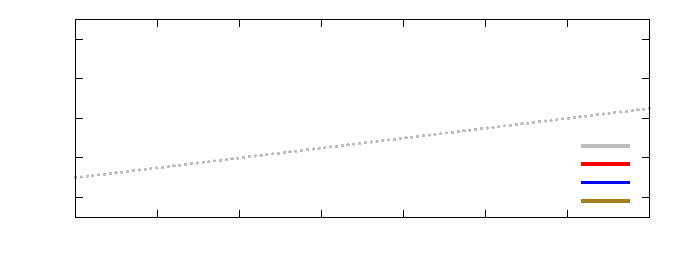
\includegraphics[width={183.00bp},height={169.00bp}]{Quinones}}%
    \gplfronttext
  \end{picture}%
\endgroup

  \caption{Graphical comparison of RI-CC2 methods for quinones. Each point is represented by the compound number given in Table \ref{tab:Quinones}. The dashed line indicates the reference CCSD(T)+E\textsubscript{CBS} values.}
  \label{fig:Quinones}
\end{figure}
  
The performance of EA-EOM-CC2 in calculating the VBS of quinones is benchmarked using a previously established test set of 10 quinones \cite{schulz2018systematic}. The results are summarised in Table \ref{tab:Quinones} and Figure \ref{fig:Quinones}. The table includes experimental adiabatic electron affinities and theoretical CCSD(T)+E\textsubscript{CBS} reference values.\\

Previous studies have demonstrated that CC2 typically performs poorly for VBSs; however, the implementation of spin-component scaling (SCS) corrections markedly enhances the accuracy of CC2 for these states \cite{paran2024performance}. The RI-CC2 results presented here include calculations both with and without SCS corrections, utilising two different basis sets: VTZ (aug-cc-pVTZ) and VDZ (aug-cc-pVDZ).\\

The incorporation of SCS improves the accuracy of CC2 for valence-bound states, corroborating the findings of Ref. \citenum{paran2024performance, shaalan2022accurate}. In general unscaled EA-EOM-RI-CC2 overbinds the electron, and the inclusion of SCS results in a slight underbinding. When comparing the results to experimental data, CC2 might appear to provide better agreement than CCSD. This apparent discrepancy arises because the experimental measurements represent adiabatic electron affinities, whilst the calculations determine vertical electron affinities.\\ 

 As with the case of DBSs, a smaller cardinality leads to a cancellation of errors in the CC2 binding energies, resulting in apparently more exact results (though arising from more inaccurate calculations). Regarding the inclusion of the extremely diffuse functions necessary for modelling DBSs, these have no impact on the VBS energy, indicating that such functions do not contribute to the description of the VBS. Of course, it is still necessary to use augmented basis sets to ensure that the VBS is well described, as the electron density of the VBS is more diffuse than that of the neutral molecule.\\

 It is noteworthy, however, that in all cases, the CC2 method reproduces the correct trend, as illustrated in Figure \ref{fig:Quinones}. The error introduced remains remarkably consistent across different molecules. Subsequent calculations omit SCS, as both DBS and VBS states can be obtained from the same Hamiltonian; one can expect a systematic overbinding of $\mathrm{\sim}$0.2 eV ensuring consistency in the results. It is also important to note that DBS predictions are known to deteriorate significantly when SCS is applied \cite{paran2024performance}, and therefore it is not a desirable method for this work. 

%This is explained by the nature of the DBS; the additional electron is situated far from the core electrons, resulting in a substantially weaker exchange interaction compared to the Coulomb interaction. This characteristic diminishes the effectiveness of SCS for such systems.

\subsection{Photoelectron Cross-section from EOM-CC2/CCSD}\label{sec:results:crosssection}

As a part of this work, Dyson orbitals between EOM-CC2 states have been implemented within the \texttt{ccman2} module of the \textit{Q-Chem} software package. To evaluate their quality, one must go beyond mere visual assessment.\\

Photodetachment cross-sections for 24 valence bound and dipole bound states were calculated using the \textit{ezDyson} package \cite{gozem2022ezspectra,gozem2015photoionization}. These calculations employ orbitals from three different sources: EOM-CC2 Dyson orbitals, EOM-CCSD Dyson orbitals and the dominant Hartree-Fock orbital. The complete results can be found in appendix \ref{ch:appendix:crosssection}. Figure \ref{fig:ezDyson} shows two representative examples: the valence bound state of azulene and the dipole bound state of nitromethane.\\

The results demonstrate  that EOM-CC2 successfully captures the essential features of the cross-section, appearing nearly identical in the case of nitromethane's dipole-bound state and showing only minor deviations for azulene. In contrast, using HF orbitals as approximations for Dyson orbitals fails to reproduce the shape obtained with EOM-CCSD. Although a single HF orbital typically dominates the Dyson orbital \cite{diaz2019dyson}, the contributions from additional electronic configurations introduced by the correlation prove to be significant.

\begin{figure}[th!]
    \centering
    \small
    % GNUPLOT: LaTeX picture with Postscript
\begingroup
  \makeatletter
  \providecommand\color[2][]{%
    \GenericError{(gnuplot) \space\space\space\@spaces}{%
      Package color not loaded in conjunction with
      terminal option `colourtext'%
    }{See the gnuplot documentation for explanation.%
    }{Either use 'blacktext' in gnuplot or load the package
      color.sty in LaTeX.}%
    \renewcommand\color[2][]{}%
  }%
  \providecommand\includegraphics[2][]{%
    \GenericError{(gnuplot) \space\space\space\@spaces}{%
      Package graphicx or graphics not loaded%
    }{See the gnuplot documentation for explanation.%
    }{The gnuplot epslatex terminal needs graphicx.sty or graphics.sty.}%
    \renewcommand\includegraphics[2][]{}%
  }%
  \providecommand\rotatebox[2]{#2}%
  \@ifundefined{ifGPcolor}{%
    \newif\ifGPcolor
    \GPcolortrue
  }{}%
  \@ifundefined{ifGPblacktext}{%
    \newif\ifGPblacktext
    \GPblacktexttrue
  }{}%
  % define a \g@addto@macro without @ in the name:
  \let\gplgaddtomacro\g@addto@macro
  % define empty templates for all commands taking text:
  \gdef\gplbacktext{}%
  \gdef\gplfronttext{}%
  \makeatother
  \ifGPblacktext
    % no textcolor at all
    \def\colorrgb#1{}%
    \def\colorgray#1{}%
  \else
    % gray or color?
    \ifGPcolor
      \def\colorrgb#1{\color[rgb]{#1}}%
      \def\colorgray#1{\color[gray]{#1}}%
      \expandafter\def\csname LTw\endcsname{\color{white}}%
      \expandafter\def\csname LTb\endcsname{\color{black}}%
      \expandafter\def\csname LTa\endcsname{\color{black}}%
      \expandafter\def\csname LT0\endcsname{\color[rgb]{1,0,0}}%
      \expandafter\def\csname LT1\endcsname{\color[rgb]{0,1,0}}%
      \expandafter\def\csname LT2\endcsname{\color[rgb]{0,0,1}}%
      \expandafter\def\csname LT3\endcsname{\color[rgb]{1,0,1}}%
      \expandafter\def\csname LT4\endcsname{\color[rgb]{0,1,1}}%
      \expandafter\def\csname LT5\endcsname{\color[rgb]{1,1,0}}%
      \expandafter\def\csname LT6\endcsname{\color[rgb]{0,0,0}}%
      \expandafter\def\csname LT7\endcsname{\color[rgb]{1,0.3,0}}%
      \expandafter\def\csname LT8\endcsname{\color[rgb]{0.5,0.5,0.5}}%
    \else
      % gray
      \def\colorrgb#1{\color{black}}%
      \def\colorgray#1{\color[gray]{#1}}%
      \expandafter\def\csname LTw\endcsname{\color{white}}%
      \expandafter\def\csname LTb\endcsname{\color{black}}%
      \expandafter\def\csname LTa\endcsname{\color{black}}%
      \expandafter\def\csname LT0\endcsname{\color{black}}%
      \expandafter\def\csname LT1\endcsname{\color{black}}%
      \expandafter\def\csname LT2\endcsname{\color{black}}%
      \expandafter\def\csname LT3\endcsname{\color{black}}%
      \expandafter\def\csname LT4\endcsname{\color{black}}%
      \expandafter\def\csname LT5\endcsname{\color{black}}%
      \expandafter\def\csname LT6\endcsname{\color{black}}%
      \expandafter\def\csname LT7\endcsname{\color{black}}%
      \expandafter\def\csname LT8\endcsname{\color{black}}%
    \fi
  \fi
    \setlength{\unitlength}{0.0500bp}%
    \ifx\gptboxheight\undefined%
      \newlength{\gptboxheight}%
      \newlength{\gptboxwidth}%
      \newsavebox{\gptboxtext}%
    \fi%
    \setlength{\fboxrule}{0.5pt}%
    \setlength{\fboxsep}{1pt}%
    \definecolor{tbcol}{rgb}{1,1,1}%
\begin{picture}(6980.00,3480.00)%
    \gplgaddtomacro\gplbacktext{%
      \csname LTb\endcsname%%
      \put(598,519){\makebox(0,0)[r]{\strut{}$0$}}%
      \csname LTb\endcsname%%
      \put(598,806){\makebox(0,0)[r]{\strut{}$2$}}%
      \csname LTb\endcsname%%
      \put(598,1093){\makebox(0,0)[r]{\strut{}$4$}}%
      \csname LTb\endcsname%%
      \put(598,1380){\makebox(0,0)[r]{\strut{}$6$}}%
      \csname LTb\endcsname%%
      \put(598,1667){\makebox(0,0)[r]{\strut{}$8$}}%
      \csname LTb\endcsname%%
      \put(598,1954){\makebox(0,0)[r]{\strut{}$10$}}%
      \csname LTb\endcsname%%
      \put(598,2242){\makebox(0,0)[r]{\strut{}$12$}}%
      \csname LTb\endcsname%%
      \put(598,2529){\makebox(0,0)[r]{\strut{}$14$}}%
      \csname LTb\endcsname%%
      \put(598,2816){\makebox(0,0)[r]{\strut{}$16$}}%
      \csname LTb\endcsname%%
      \put(598,3103){\makebox(0,0)[r]{\strut{}$18$}}%
      \csname LTb\endcsname%%
      \put(598,3390){\makebox(0,0)[r]{\strut{}$20$}}%
      \csname LTb\endcsname%%
      \put(696,343){\makebox(0,0){\strut{}$0$}}%
      \csname LTb\endcsname%%
      \put(1252,343){\makebox(0,0){\strut{}$2$}}%
      \csname LTb\endcsname%%
      \put(1809,343){\makebox(0,0){\strut{}$4$}}%
      \csname LTb\endcsname%%
      \put(2366,343){\makebox(0,0){\strut{}$6$}}%
      \csname LTb\endcsname%%
      \put(2923,343){\makebox(0,0){\strut{}$8$}}%
      \csname LTb\endcsname%%
      \put(3479,343){\makebox(0,0){\strut{}$10$}}%
    }%
    \gplgaddtomacro\gplfronttext{%
      \csname LTb\endcsname%%
      \put(2790,3135){\makebox(0,0)[r]{\strut{}CC2}}%
      \csname LTb\endcsname%%
      \put(2790,2959){\makebox(0,0)[r]{\strut{}CCSD}}%
      \csname LTb\endcsname%%
      \put(2790,2783){\makebox(0,0)[r]{\strut{}HF}}%
      \csname LTb\endcsname%%
      \put(240,1954){\rotatebox{-270.00}{\makebox(0,0){\strut{}X sec  (a.u.)}}}%
      \csname LTb\endcsname%%
      \put(2087,79){\makebox(0,0){\strut{}$\mathrm{E_I+E_k}$ (eV)}}%
    }%
    \gplgaddtomacro\gplbacktext{%
      \csname LTb\endcsname%%
      \put(3938,519){\makebox(0,0)[r]{\strut{}$0$}}%
      \csname LTb\endcsname%%
      \put(3938,997){\makebox(0,0)[r]{\strut{}$200$}}%
      \csname LTb\endcsname%%
      \put(3938,1476){\makebox(0,0)[r]{\strut{}$400$}}%
      \csname LTb\endcsname%%
      \put(3938,1954){\makebox(0,0)[r]{\strut{}$600$}}%
      \csname LTb\endcsname%%
      \put(3938,2433){\makebox(0,0)[r]{\strut{}$800$}}%
      \csname LTb\endcsname%%
      \put(3938,2912){\makebox(0,0)[r]{\strut{}$1000$}}%
      \csname LTb\endcsname%%
      \put(3938,3390){\makebox(0,0)[r]{\strut{}$1200$}}%
      \csname LTb\endcsname%%
      \put(4036,343){\makebox(0,0){\strut{}$0$}}%
      \csname LTb\endcsname%%
      \put(4732,343){\makebox(0,0){\strut{}$0.5$}}%
      \csname LTb\endcsname%%
      \put(5428,343){\makebox(0,0){\strut{}$1$}}%
      \csname LTb\endcsname%%
      \put(6124,343){\makebox(0,0){\strut{}$1.5$}}%
      \csname LTb\endcsname%%
      \put(6820,343){\makebox(0,0){\strut{}$2$}}%
    }%
    \gplgaddtomacro\gplfronttext{%
      \csname LTb\endcsname%%
      \put(6130,3135){\makebox(0,0)[r]{\strut{}CC2}}%
      \csname LTb\endcsname%%
      \put(6130,2959){\makebox(0,0)[r]{\strut{}CCSD}}%
      \csname LTb\endcsname%%
      \put(6130,2783){\makebox(0,0)[r]{\strut{}HF}}%
      \csname LTb\endcsname%%
      \put(5428,79){\makebox(0,0){\strut{}$\mathrm{E_I+E_k}$ (eV)}}%
    }%
    \gplbacktext
    \put(0,0){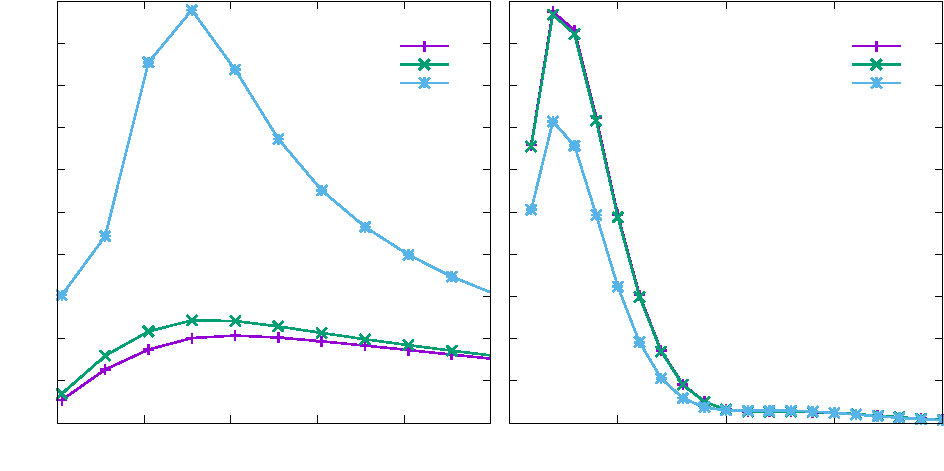
\includegraphics[width={349.00bp},height={174.00bp}]{ezDyson}}%
    \gplfronttext
    \put(1150,1350){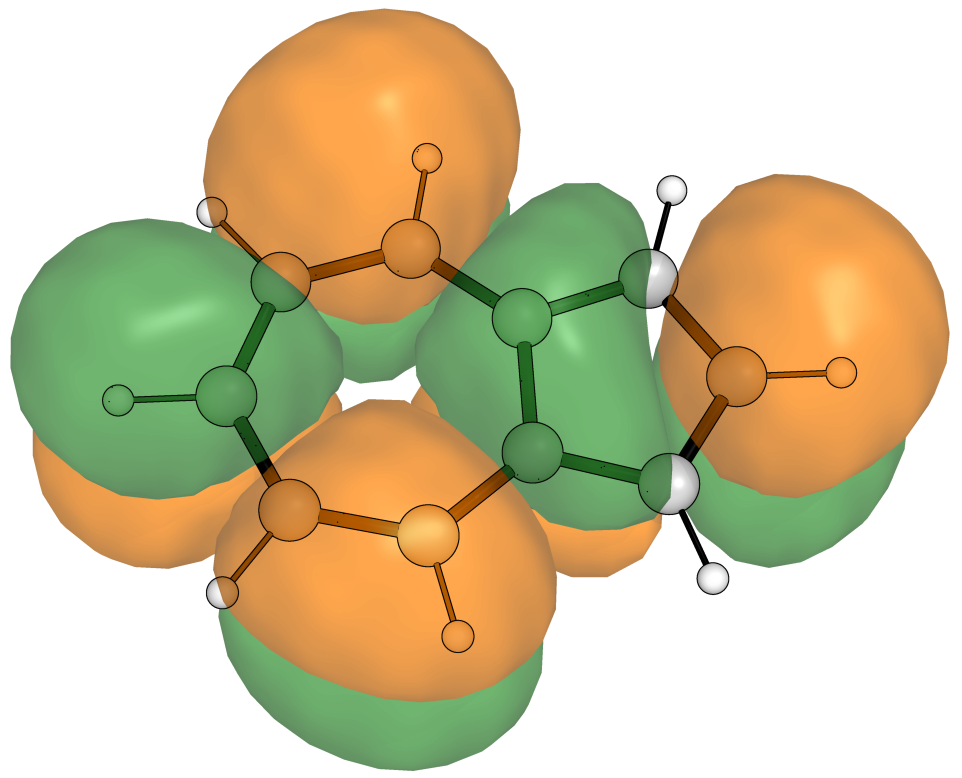
\includegraphics[scale=0.27]{azulene.png}}%
    \put(5100,1300){\includegraphics[scale=0.45]{../../introduction/image/MeNO2_DBS.png}}%
  \end{picture}%
\endgroup

    %figsize is set in image/test.gp 
    \caption[Photoedetachment Crossections.]{ Photoedetachment cross-sections of azulene (VBS) and nitromethane (DBS). The cross-sections were calculated using Dyson orbitals from EOM-CC2, EOM-CCSD and the dominant HF orbital in the EOM-CCSD Dyson orbital. The corresponding EA-EOM-CC2 Dyson orbitals are also shown as insets.}
    \label{fig:ezDyson}
\end{figure}

\section{Study on the Anion States of Ubiquinone}

Once the performance of the methods has been assessed, the focus shifts to the anion states of ubiquinone (CoQ). All results presented here are based on the calculations performed with RI-EA-EOM-CC/aug-cc-pVDZ+6s3p unless specified otherwise.

\subsection{Energy and Dipole Surfaces of CoQ}

\subsubsection{Surfaces of Q0}

The conformational landscape of the simplest ubiquinone, Q\textsubscript{0}, was investigated by varying the dihedral angles of the methoxy chains relative to the quinone plane in steps of 20\degree, as shown in Figure \ref{fig:Q0_dyson}. These dihedral angles represent the most significant degrees of freedom in the system, as the remainder of the molecule is relatively rigid. This approach enables the construction of potential energy surfaces (PES), dipole strength surfaces, and PES for the anionic states (VBS and DBS), as depicted in Figure \ref{fig:Q0_maps}. Owing to the C\textsubscript{2} symmetry present when the methoxy chains are coplanar, only half of the surface points require sampling.\\
\begin{figure}[b!]
  \centering
  \begin{minipage}[b]{0.30\textwidth}
    \centering
    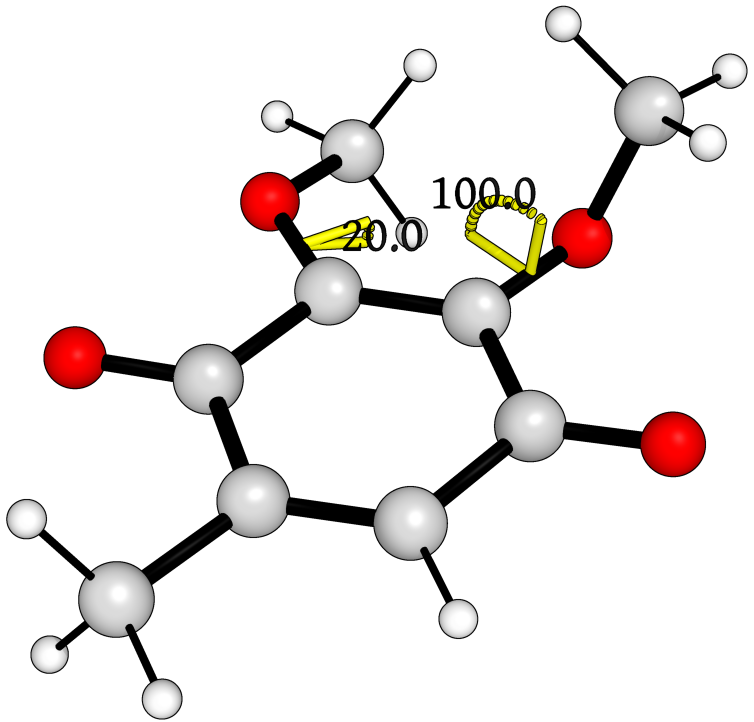
\includegraphics[width=1.15\textwidth]{chapters/results/image/dihedrals.png}
    \vspace{15pt}
    \small\emph{Methoxy dihedrals}
  \end{minipage}
  \hfill
  \begin{minipage}[b]{0.30\textwidth}
    \centering
      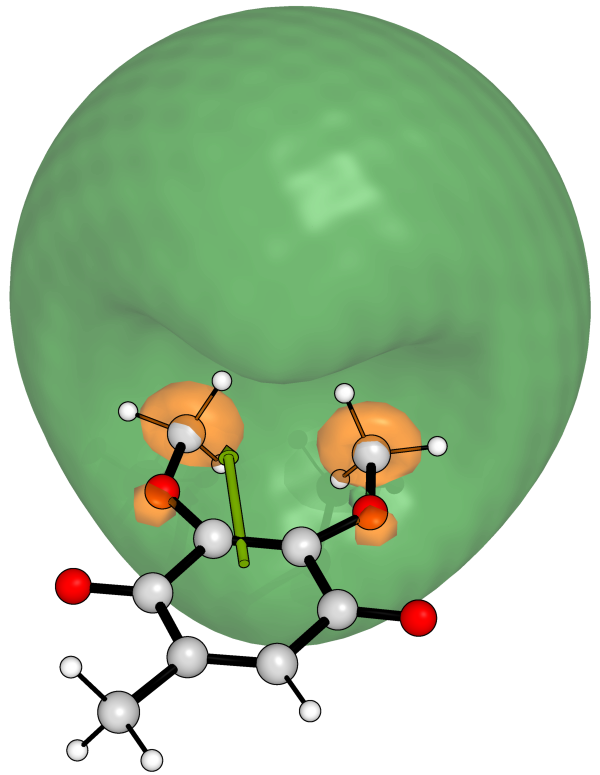
\includegraphics[width=0.8\textwidth]{chapters/results/image/Q0_181.png}
      \small\emph{Region A \\ $(0,0)~\mu=2.5~D$ E=15.8~meV}
  \end{minipage}
  \hfill
  \begin{minipage}[b]{0.30\textwidth}
    \centering
      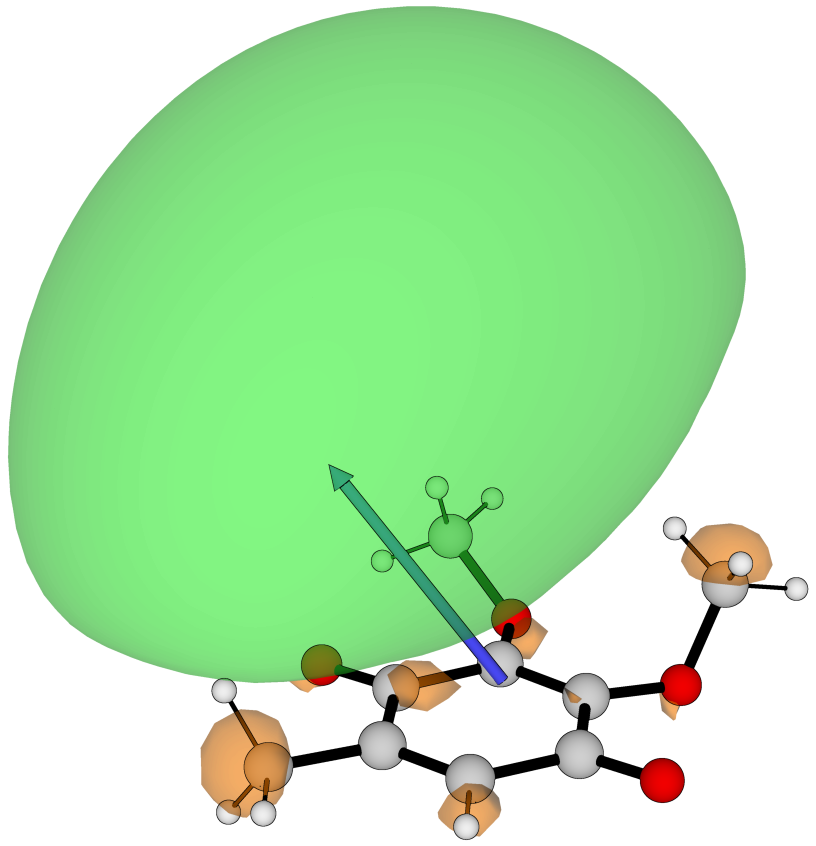
\includegraphics[width=\textwidth]{chapters/results/image/Q0_52.png}
      \small\emph{Region B $(\pm140,\mp20)~\mu=3.2~D$, $E=6.2~meV$}
  \end{minipage}
  \caption[Dyson orbitals of Q0]{Dyson orbitals of Q0 calculated with RI-EA-EOM-CC2/aug-cc-pVDZ+6s3p. The left panel explicitly shows the methoxy dihedral coordinates. The middle panel shows the Dyson orbital of the strongest bound DBS from region B. The right panel shows the Dyson orbital strongest bound DBS from region A. The isosurface is set to 0.005 a.u. and the dipole moment vector is shown as a green arrow with origin at the centre of mass.}
  \label{fig:Q0_dyson}
\end{figure}

\begin{figure}[b!]
  \centering
  \small
  % GNUPLOT: LaTeX picture with Postscript
\begingroup
  \makeatletter
  \providecommand\color[2][]{%
    \GenericError{(gnuplot) \space\space\space\@spaces}{%
      Package color not loaded in conjunction with
      terminal option `colourtext'%
    }{See the gnuplot documentation for explanation.%
    }{Either use 'blacktext' in gnuplot or load the package
      color.sty in LaTeX.}%
    \renewcommand\color[2][]{}%
  }%
  \providecommand\includegraphics[2][]{%
    \GenericError{(gnuplot) \space\space\space\@spaces}{%
      Package graphicx or graphics not loaded%
    }{See the gnuplot documentation for explanation.%
    }{The gnuplot epslatex terminal needs graphicx.sty or graphics.sty.}%
    \renewcommand\includegraphics[2][]{}%
  }%
  \providecommand\rotatebox[2]{#2}%
  \@ifundefined{ifGPcolor}{%
    \newif\ifGPcolor
    \GPcolortrue
  }{}%
  \@ifundefined{ifGPblacktext}{%
    \newif\ifGPblacktext
    \GPblacktexttrue
  }{}%
  % define a \g@addto@macro without @ in the name:
  \let\gplgaddtomacro\g@addto@macro
  % define empty templates for all commands taking text:
  \gdef\gplbacktext{}%
  \gdef\gplfronttext{}%
  \makeatother
  \ifGPblacktext
    % no textcolor at all
    \def\colorrgb#1{}%
    \def\colorgray#1{}%
  \else
    % gray or color?
    \ifGPcolor
      \def\colorrgb#1{\color[rgb]{#1}}%
      \def\colorgray#1{\color[gray]{#1}}%
      \expandafter\def\csname LTw\endcsname{\color{white}}%
      \expandafter\def\csname LTb\endcsname{\color{black}}%
      \expandafter\def\csname LTa\endcsname{\color{black}}%
      \expandafter\def\csname LT0\endcsname{\color[rgb]{1,0,0}}%
      \expandafter\def\csname LT1\endcsname{\color[rgb]{0,1,0}}%
      \expandafter\def\csname LT2\endcsname{\color[rgb]{0,0,1}}%
      \expandafter\def\csname LT3\endcsname{\color[rgb]{1,0,1}}%
      \expandafter\def\csname LT4\endcsname{\color[rgb]{0,1,1}}%
      \expandafter\def\csname LT5\endcsname{\color[rgb]{1,1,0}}%
      \expandafter\def\csname LT6\endcsname{\color[rgb]{0,0,0}}%
      \expandafter\def\csname LT7\endcsname{\color[rgb]{1,0.3,0}}%
      \expandafter\def\csname LT8\endcsname{\color[rgb]{0.5,0.5,0.5}}%
    \else
      % gray
      \def\colorrgb#1{\color{black}}%
      \def\colorgray#1{\color[gray]{#1}}%
      \expandafter\def\csname LTw\endcsname{\color{white}}%
      \expandafter\def\csname LTb\endcsname{\color{black}}%
      \expandafter\def\csname LTa\endcsname{\color{black}}%
      \expandafter\def\csname LT0\endcsname{\color{black}}%
      \expandafter\def\csname LT1\endcsname{\color{black}}%
      \expandafter\def\csname LT2\endcsname{\color{black}}%
      \expandafter\def\csname LT3\endcsname{\color{black}}%
      \expandafter\def\csname LT4\endcsname{\color{black}}%
      \expandafter\def\csname LT5\endcsname{\color{black}}%
      \expandafter\def\csname LT6\endcsname{\color{black}}%
      \expandafter\def\csname LT7\endcsname{\color{black}}%
      \expandafter\def\csname LT8\endcsname{\color{black}}%
    \fi
  \fi
    \setlength{\unitlength}{0.0500bp}%
    \ifx\gptboxheight\undefined%
      \newlength{\gptboxheight}%
      \newlength{\gptboxwidth}%
      \newsavebox{\gptboxtext}%
    \fi%
    \setlength{\fboxrule}{0.5pt}%
    \setlength{\fboxsep}{1pt}%
    \definecolor{tbcol}{rgb}{1,1,1}%
\begin{picture}(9060.00,9060.00)%
    \gplgaddtomacro\gplbacktext{%
    }%
    \gplgaddtomacro\gplfronttext{%
      \csname LTb\endcsname%%
      \put(444,5102){\makebox(0,0)[r]{\strut{}$-160$}}%
      \csname LTb\endcsname%%
      \put(444,5544){\makebox(0,0)[r]{\strut{}$-120$}}%
      \csname LTb\endcsname%%
      \put(444,5986){\makebox(0,0)[r]{\strut{}$-80$}}%
      \csname LTb\endcsname%%
      \put(444,6428){\makebox(0,0)[r]{\strut{}$-40$}}%
      \csname LTb\endcsname%%
      \put(444,6870){\makebox(0,0)[r]{\strut{}$0$}}%
      \csname LTb\endcsname%%
      \put(444,7312){\makebox(0,0)[r]{\strut{}$40$}}%
      \csname LTb\endcsname%%
      \put(444,7754){\makebox(0,0)[r]{\strut{}$80$}}%
      \csname LTb\endcsname%%
      \put(444,8196){\makebox(0,0)[r]{\strut{}$120$}}%
      \csname LTb\endcsname%%
      \put(444,8638){\makebox(0,0)[r]{\strut{}$160$}}%
      \csname LTb\endcsname%%
      \put(542,4705){\makebox(0,0){\strut{}}}%
      \csname LTb\endcsname%%
      \put(1205,4705){\makebox(0,0){\strut{}}}%
      \csname LTb\endcsname%%
      \put(1868,4705){\makebox(0,0){\strut{}}}%
      \csname LTb\endcsname%%
      \put(2531,4705){\makebox(0,0){\strut{}}}%
      \csname LTb\endcsname%%
      \put(3194,4705){\makebox(0,0){\strut{}}}%
      \csname LTb\endcsname%%
      \put(3857,4705){\makebox(0,0){\strut{}}}%
      \csname LTb\endcsname%%
      \put(4520,4705){\makebox(0,0){\strut{}}}%
      \csname LTb\endcsname%%
      \put(87,6870){\rotatebox{-270.00}{\makebox(0,0){\normalsize $\Psi$}}}%
      \csname LTb\endcsname%%
      \put(2089,7154){\rotatebox{-66.00}{\makebox(0,0){\strut{}\textcolor{black}{\footnotesize 500}}}}%
      \csname LTb\endcsname%%
      \put(2907,6987){\rotatebox{130.00}{\makebox(0,0){\strut{}\textcolor{black}{\footnotesize 400}}}}%
      \csname LTb\endcsname%%
      \put(2146,6682){\rotatebox{-27.00}{\makebox(0,0){\strut{}\textcolor{black}{\footnotesize 400}}}}%
      \csname LTb\endcsname%%
      \put(2313,7650){\rotatebox{154.00}{\makebox(0,0){\strut{}\textcolor{black}{\footnotesize 300}}}}%
      \csname LTb\endcsname%%
      \put(2302,6385){\rotatebox{-39.00}{\makebox(0,0){\strut{}\textcolor{black}{\footnotesize 300}}}}%
      \csname LTb\endcsname%%
      \put(3383,6779){\rotatebox{113.00}{\makebox(0,0){\strut{}\textcolor{black}{\footnotesize 200}}}}%
      \csname LTb\endcsname%%
      \put(1472,8023){\rotatebox{-143.00}{\makebox(0,0){\strut{}\textcolor{black}{\footnotesize 200}}}}%
      \csname LTb\endcsname%%
      \put(2514,6042){\rotatebox{-26.00}{\makebox(0,0){\strut{}\textcolor{black}{\footnotesize 200}}}}%
      \csname LTb\endcsname%%
      \put(1231,8224){\rotatebox{39.00}{\makebox(0,0){\strut{}\textcolor{black}{\footnotesize 100}}}}%
      \csname LTb\endcsname%%
      \put(3216,8239){\rotatebox{42.00}{\makebox(0,0){\strut{}\textcolor{black}{\footnotesize 100}}}}%
      \csname LTb\endcsname%%
      \put(3517,6877){\rotatebox{-71.00}{\makebox(0,0){\strut{}\textcolor{black}{\footnotesize 100}}}}%
      \csname LTb\endcsname%%
      \put(1307,7421){\rotatebox{-43.00}{\makebox(0,0){\strut{}\textcolor{black}{\footnotesize 100}}}}%
      \csname LTb\endcsname%%
      \put(1378,5563){\rotatebox{-33.00}{\makebox(0,0){\strut{}\textcolor{black}{\footnotesize 100}}}}%
      \csname LTb\endcsname%%
      \put(3383,5294){\rotatebox{-28.00}{\makebox(0,0){\strut{}\textcolor{black}{\footnotesize 100}}}}%
      \csname LTb\endcsname%%
      \put(705,7288){\rotatebox{-112.00}{\makebox(0,0){\strut{}\textcolor{black}{\footnotesize 50}}}}%
      \csname LTb\endcsname%%
      \put(3758,7221){\rotatebox{-149.00}{\makebox(0,0){\strut{}\textcolor{black}{\footnotesize 50}}}}%
      \csname LTb\endcsname%%
      \put(2213,8126){\rotatebox{-28.00}{\makebox(0,0){\strut{}\textcolor{black}{\footnotesize 50}}}}%
      \csname LTb\endcsname%%
      \put(2292,5650){\rotatebox{31.00}{\makebox(0,0){\strut{}\textcolor{black}{\footnotesize 50}}}}%
      \csname LTb\endcsname%%
      \put(2531,8982){\makebox(0,0){\strut{}Conformational Energy (meV)}}%
    }%
    \gplgaddtomacro\gplbacktext{%
    }%
    \gplgaddtomacro\gplfronttext{%
      \csname LTb\endcsname%%
      \put(4874,5102){\makebox(0,0)[r]{\strut{}}}%
      \csname LTb\endcsname%%
      \put(4874,5544){\makebox(0,0)[r]{\strut{}}}%
      \csname LTb\endcsname%%
      \put(4874,5986){\makebox(0,0)[r]{\strut{}}}%
      \csname LTb\endcsname%%
      \put(4874,6428){\makebox(0,0)[r]{\strut{}}}%
      \csname LTb\endcsname%%
      \put(4874,6870){\makebox(0,0)[r]{\strut{}}}%
      \csname LTb\endcsname%%
      \put(4874,7312){\makebox(0,0)[r]{\strut{}}}%
      \csname LTb\endcsname%%
      \put(4874,7754){\makebox(0,0)[r]{\strut{}}}%
      \csname LTb\endcsname%%
      \put(4874,8196){\makebox(0,0)[r]{\strut{}}}%
      \csname LTb\endcsname%%
      \put(4874,8638){\makebox(0,0)[r]{\strut{}}}%
      \csname LTb\endcsname%%
      \put(4971,4705){\makebox(0,0){\strut{}}}%
      \csname LTb\endcsname%%
      \put(5634,4705){\makebox(0,0){\strut{}}}%
      \csname LTb\endcsname%%
      \put(6297,4705){\makebox(0,0){\strut{}}}%
      \csname LTb\endcsname%%
      \put(6960,4705){\makebox(0,0){\strut{}}}%
      \csname LTb\endcsname%%
      \put(7623,4705){\makebox(0,0){\strut{}}}%
      \csname LTb\endcsname%%
      \put(8286,4705){\makebox(0,0){\strut{}}}%
      \csname LTb\endcsname%%
      \put(8949,4705){\makebox(0,0){\strut{}}}%
      \csname LTb\endcsname%%
      \put(5031,7851){\rotatebox{37.00}{\makebox(0,0){\strut{}\textcolor{black}{\footnotesize 3.0}}}}%
      \csname LTb\endcsname%%
      \put(8832,6500){\rotatebox{156.00}{\makebox(0,0){\strut{}\textcolor{black}{\footnotesize 3.0}}}}%
      \csname LTb\endcsname%%
      \put(6547,7260){\rotatebox{-78.00}{\makebox(0,0){\strut{}\textcolor{black}{\footnotesize 2.5}}}}%
      \csname LTb\endcsname%%
      \put(5651,8271){\rotatebox{-7.00}{\makebox(0,0){\strut{}\textcolor{black}{\footnotesize 2.5}}}}%
      \csname LTb\endcsname%%
      \put(5409,6940){\rotatebox{-127.00}{\makebox(0,0){\strut{}\textcolor{black}{\footnotesize 2.5}}}}%
      \csname LTb\endcsname%%
      \put(8618,7519){\rotatebox{-88.00}{\makebox(0,0){\strut{}\textcolor{black}{\footnotesize 2.5}}}}%
      \csname LTb\endcsname%%
      \put(8083,6140){\rotatebox{-101.00}{\makebox(0,0){\strut{}\textcolor{black}{\footnotesize 2.5}}}}%
      \csname LTb\endcsname%%
      \put(5500,6320){\rotatebox{91.00}{\makebox(0,0){\strut{}\textcolor{black}{\footnotesize 2.0}}}}%
      \csname LTb\endcsname%%
      \put(6314,7040){\rotatebox{-47.00}{\makebox(0,0){\strut{}\textcolor{black}{\footnotesize 2.0}}}}%
      \csname LTb\endcsname%%
      \put(7233,6000){\rotatebox{-38.00}{\makebox(0,0){\strut{}\textcolor{black}{\footnotesize 2.0}}}}%
      \csname LTb\endcsname%%
      \put(6531,7999){\rotatebox{-101.00}{\makebox(0,0){\strut{}\textcolor{black}{\footnotesize 2.0}}}}%
      \csname LTb\endcsname%%
      \put(7425,6960){\rotatebox{-59.00}{\makebox(0,0){\strut{}\textcolor{black}{\footnotesize 2.0}}}}%
      \csname LTb\endcsname%%
      \put(8359,7080){\rotatebox{64.00}{\makebox(0,0){\strut{}\textcolor{black}{\footnotesize 2.0}}}}%
      \csname LTb\endcsname%%
      \put(5471,5690){\rotatebox{52.00}{\makebox(0,0){\strut{}\textcolor{black}{\footnotesize 1.5}}}}%
      \csname LTb\endcsname%%
      \put(6291,6706){\rotatebox{-17.00}{\makebox(0,0){\strut{}\textcolor{black}{\footnotesize 1.5}}}}%
      \csname LTb\endcsname%%
      \put(6870,5426){\rotatebox{-106.00}{\makebox(0,0){\strut{}\textcolor{black}{\footnotesize 1.5}}}}%
      \csname LTb\endcsname%%
      \put(7650,8582){\rotatebox{-176.00}{\makebox(0,0){\strut{}\textcolor{black}{\footnotesize 1.5}}}}%
      \csname LTb\endcsname%%
      \put(7238,7519){\rotatebox{-45.00}{\makebox(0,0){\strut{}\textcolor{black}{\footnotesize 1.5}}}}%
      \csname LTb\endcsname%%
      \put(8205,7420){\rotatebox{78.00}{\makebox(0,0){\strut{}\textcolor{black}{\footnotesize 1.5}}}}%
      \csname LTb\endcsname%%
      \put(5771,5854){\rotatebox{56.00}{\makebox(0,0){\strut{}\textcolor{black}{\footnotesize 1.0}}}}%
      \csname LTb\endcsname%%
      \put(6570,5482){\rotatebox{-124.00}{\makebox(0,0){\strut{}\textcolor{black}{\footnotesize 1.0}}}}%
      \csname LTb\endcsname%%
      \put(7490,8350){\rotatebox{-162.00}{\makebox(0,0){\strut{}\textcolor{black}{\footnotesize 1.0}}}}%
      \csname LTb\endcsname%%
      \put(8062,7739){\rotatebox{60.00}{\makebox(0,0){\strut{}\textcolor{black}{\footnotesize 1.0}}}}%
      \csname LTb\endcsname%%
      \put(5883,5721){\rotatebox{-132.00}{\makebox(0,0){\strut{}\textcolor{black}{\footnotesize 0.5}}}}%
      \csname LTb\endcsname%%
      \put(7669,8179){\rotatebox{-140.00}{\makebox(0,0){\strut{}\textcolor{black}{\footnotesize 0.5}}}}%
      \csname LTb\endcsname%%
      \put(6960,8982){\makebox(0,0){Dipole Strength (Debye)}}%
    }%
    \gplgaddtomacro\gplbacktext{%
    }%
    \gplgaddtomacro\gplfronttext{%
      \csname LTb\endcsname%%
      \put(444,763){\makebox(0,0)[r]{\strut{}$-160$}}%
      \csname LTb\endcsname%%
      \put(444,1205){\makebox(0,0)[r]{\strut{}$-120$}}%
      \csname LTb\endcsname%%
      \put(444,1647){\makebox(0,0)[r]{\strut{}$-80$}}%
      \csname LTb\endcsname%%
      \put(444,2089){\makebox(0,0)[r]{\strut{}$-40$}}%
      \csname LTb\endcsname%%
      \put(444,2531){\makebox(0,0)[r]{\strut{}$0$}}%
      \csname LTb\endcsname%%
      \put(444,2973){\makebox(0,0)[r]{\strut{}$40$}}%
      \csname LTb\endcsname%%
      \put(444,3415){\makebox(0,0)[r]{\strut{}$80$}}%
      \csname LTb\endcsname%%
      \put(444,3857){\makebox(0,0)[r]{\strut{}$120$}}%
      \csname LTb\endcsname%%
      \put(444,4298){\makebox(0,0)[r]{\strut{}$160$}}%
      \csname LTb\endcsname%%
      \put(542,366){\makebox(0,0){\strut{}$-180$}}%
      \csname LTb\endcsname%%
      \put(1205,366){\makebox(0,0){\strut{}$-120$}}%
      \csname LTb\endcsname%%
      \put(1868,366){\makebox(0,0){\strut{}$-60$}}%
      \csname LTb\endcsname%%
      \put(2531,366){\makebox(0,0){\strut{}$0$}}%
      \csname LTb\endcsname%%
      \put(3194,366){\makebox(0,0){\strut{}$60$}}%
      \csname LTb\endcsname%%
      \put(3857,366){\makebox(0,0){\strut{}$120$}}%
      \csname LTb\endcsname%%
      \put(4519,366){\makebox(0,0){\strut{}$180$}}%
      \csname LTb\endcsname%%
      \put(87,2531){\rotatebox{-270.00}{\makebox(0,0){\normalsize $\Psi$}}}%
      \csname LTb\endcsname%%
      \put(2531,102){\makebox(0,0){\normalsize $\Phi$}}%
      \csname LTb\endcsname%%
      \put(2390,2781){\rotatebox{150.00}{\makebox(0,0){\strut{}\textcolor{black}{\footnotesize 1.3}}}}%
      \csname LTb\endcsname%%
      \put(2270,2355){\rotatebox{-57.00}{\makebox(0,0){\strut{}\textcolor{black}{\footnotesize 1.4}}}}%
      \csname LTb\endcsname%%
      \put(2912,2859){\rotatebox{124.00}{\makebox(0,0){\strut{}\textcolor{black}{\footnotesize 1.5}}}}%
      \csname LTb\endcsname%%
      \put(2511,1819){\rotatebox{-36.00}{\makebox(0,0){\strut{}\textcolor{black}{\footnotesize 1.5}}}}%
      \csname LTb\endcsname%%
      \put(2052,3555){\rotatebox{51.00}{\makebox(0,0){\strut{}\textcolor{black}{\footnotesize 1.6}}}}%
      \csname LTb\endcsname%%
      \put(2164,1627){\rotatebox{-79.00}{\makebox(0,0){\strut{}\textcolor{black}{\footnotesize 1.6}}}}%
      \csname LTb\endcsname%%
      \put(3435,2928){\rotatebox{-15.00}{\makebox(0,0){\strut{}\textcolor{black}{\footnotesize 1.6}}}}%
      \csname LTb\endcsname%%
      \put(3530,2028){\rotatebox{40.00}{\makebox(0,0){\strut{}\textcolor{black}{\footnotesize 1.6}}}}%
      \csname LTb\endcsname%%
      \put(1814,1426){\rotatebox{-81.00}{\makebox(0,0){\strut{}\textcolor{black}{\footnotesize 1.7}}}}%
      \csname LTb\endcsname%%
      \put(1753,3676){\rotatebox{49.00}{\makebox(0,0){\strut{}\textcolor{black}{\footnotesize 1.7}}}}%
      \csname LTb\endcsname%%
      \put(3475,3295){\rotatebox{-26.00}{\makebox(0,0){\strut{}\textcolor{black}{\footnotesize 1.7}}}}%
      \csname LTb\endcsname%%
      \put(3592,1667){\rotatebox{55.00}{\makebox(0,0){\strut{}\textcolor{black}{\footnotesize 1.7}}}}%
      \csname LTb\endcsname%%
      \put(2531,4643){\makebox(0,0){VBA EA (eV)}}%
    }%
    \gplgaddtomacro\gplbacktext{%
    }%
    \gplgaddtomacro\gplfronttext{%
      \csname LTb\endcsname%%
      \put(4874,763){\makebox(0,0)[r]{\strut{}}}%
      \csname LTb\endcsname%%
      \put(4874,1205){\makebox(0,0)[r]{\strut{}}}%
      \csname LTb\endcsname%%
      \put(4874,1647){\makebox(0,0)[r]{\strut{}}}%
      \csname LTb\endcsname%%
      \put(4874,2089){\makebox(0,0)[r]{\strut{}}}%
      \csname LTb\endcsname%%
      \put(4874,2531){\makebox(0,0)[r]{\strut{}}}%
      \csname LTb\endcsname%%
      \put(4874,2973){\makebox(0,0)[r]{\strut{}}}%
      \csname LTb\endcsname%%
      \put(4874,3415){\makebox(0,0)[r]{\strut{}}}%
      \csname LTb\endcsname%%
      \put(4874,3857){\makebox(0,0)[r]{\strut{}}}%
      \csname LTb\endcsname%%
      \put(4874,4298){\makebox(0,0)[r]{\strut{}}}%
      \csname LTb\endcsname%%
      \put(4971,366){\makebox(0,0){\strut{}$-180$}}%
      \csname LTb\endcsname%%
      \put(5634,366){\makebox(0,0){\strut{}$-120$}}%
      \csname LTb\endcsname%%
      \put(6297,366){\makebox(0,0){\strut{}$-60$}}%
      \csname LTb\endcsname%%
      \put(6960,366){\makebox(0,0){\strut{}$0$}}%
      \csname LTb\endcsname%%
      \put(7623,366){\makebox(0,0){\strut{}$60$}}%
      \csname LTb\endcsname%%
      \put(8286,366){\makebox(0,0){\strut{}$120$}}%
      \csname LTb\endcsname%%
      \put(8949,366){\makebox(0,0){\strut{}$180$}}%
      \csname LTb\endcsname%%
      \put(6960,102){\makebox(0,0){\normalsize $\Phi$}}%
      \csname LTb\endcsname%%
      \put(7021,2310){\rotatebox{-43.00}{\makebox(0,0){\strut{}\textcolor{black}{\footnotesize 12}}}}%
      \csname LTb\endcsname%%
      \put(7236,2069){\rotatebox{-30.00}{\makebox(0,0){\strut{}\textcolor{black}{\footnotesize 9}}}}%
      \csname LTb\endcsname%%
      \put(5255,3234){\rotatebox{-53.00}{\makebox(0,0){\strut{}\textcolor{black}{\footnotesize 6}}}}%
      \csname LTb\endcsname%%
      \put(7107,2792){\rotatebox{130.00}{\makebox(0,0){\strut{}\textcolor{black}{\footnotesize 6}}}}%
      \csname LTb\endcsname%%
      \put(7422,1854){\rotatebox{-23.00}{\makebox(0,0){\strut{}\textcolor{black}{\footnotesize 6}}}}%
      \csname LTb\endcsname%%
      \put(8467,1607){\rotatebox{-42.00}{\makebox(0,0){\strut{}\textcolor{black}{\footnotesize 6}}}}%
      \csname LTb\endcsname%%
      \put(7686,2189){\rotatebox{113.00}{\makebox(0,0){\strut{}\textcolor{black}{\footnotesize 3}}}}%
      \csname LTb\endcsname%%
      \put(5496,3877){\rotatebox{-170.00}{\makebox(0,0){\strut{}\textcolor{black}{\footnotesize 3}}}}%
      \csname LTb\endcsname%%
      \put(6531,2591){\rotatebox{-35.00}{\makebox(0,0){\strut{}\textcolor{black}{\footnotesize 3}}}}%
      \csname LTb\endcsname%%
      \put(8748,1369){\rotatebox{50.00}{\makebox(0,0){\strut{}\textcolor{black}{\footnotesize 3}}}}%
      \csname LTb\endcsname%%
      \put(5107,1627){\rotatebox{-108.00}{\makebox(0,0){\strut{}\textcolor{black}{\footnotesize 0}}}}%
      \csname LTb\endcsname%%
      \put(8798,2912){\rotatebox{-74.00}{\makebox(0,0){\strut{}\textcolor{black}{\footnotesize 0}}}}%
      \csname LTb\endcsname%%
      \put(6538,3598){\rotatebox{-62.00}{\makebox(0,0){\strut{}\textcolor{black}{\footnotesize 0}}}}%
      \csname LTb\endcsname%%
      \put(8748,2534){\rotatebox{3.00}{\makebox(0,0){\strut{}\textcolor{black}{\footnotesize 0}}}}%
      \csname LTb\endcsname%%
      \put(6568,2390){\rotatebox{-68.00}{\makebox(0,0){\strut{}\textcolor{black}{\footnotesize 0}}}}%
      \csname LTb\endcsname%%
      \put(8788,1198){\rotatebox{47.00}{\makebox(0,0){\strut{}\textcolor{black}{\footnotesize 0}}}}%
      \csname LTb\endcsname%%
      \put(5767,2531){\makebox(0,0){\strut{}\textcolor{black}{\normalsize \textbf{B}}}}%
      \csname LTb\endcsname%%
      \put(8153,2531){\makebox(0,0){\strut{}\textcolor{black}{\normalsize \textbf{B}}}}%
      \csname LTb\endcsname%%
      \put(6483,2133){\makebox(0,0){\strut{}\textcolor{black}{\normalsize \textbf{A}}}}%
      \csname LTb\endcsname%%
      \put(6960,4643){\makebox(0,0){DBA EA (meV)}}%
    }%
    \gplbacktext
    \put(0,0){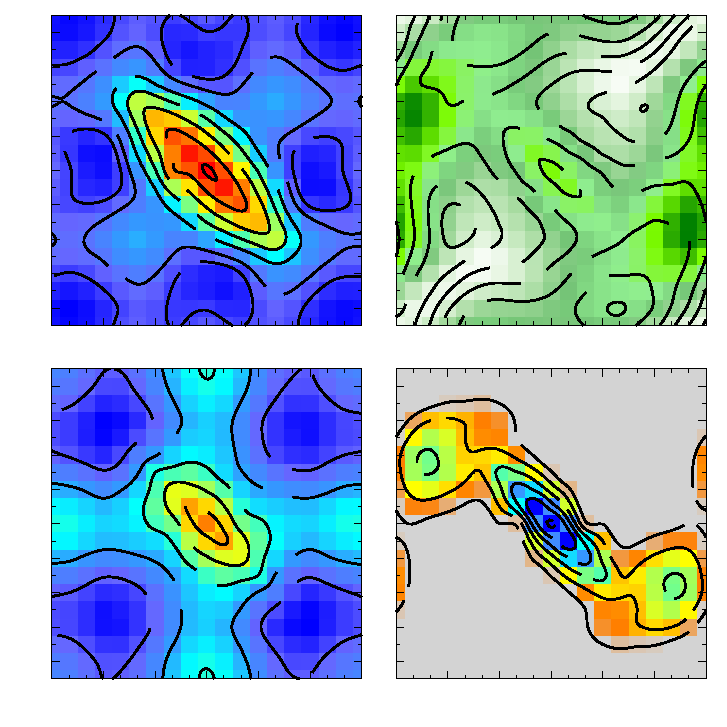
\includegraphics[width={453.00bp},height={453.00bp}]{chapters/results/image/Q0_maps}}%
    \gplfronttext
  \end{picture}%
\endgroup
 
  \caption[Surfaces of Q0]{Surfaces of Q0. From left to right and top to bottom: potential energy surface (CC2), dipole strength surface (DFT TPSS), PES for the VBS (EA-EOM-CC2), and PES for the DBS (EA-EOM-CC2). Gray points the DBS surface indicate that the DBS is not predicted to exist.\label{fig:Q0_maps}}
\end{figure}

The conformational energy surface of the neutral molecule reveals five minima, corresponding to configurations where the methoxy groups are oriented away from each other. The global minimum occurs at (180,180), where both chains are coplanar with the quinone and directed oppositely. Four additional minima are found at $\mathrm{(\pm140,\mp20)}$ and $\mathrm{(\pm20,\mp140)}$, each approximately 10 meV above the global minimum. The presence of a methyl group at position 5 slightly perturbs the symmetry between the methoxy chains, but its influence on the energy landscape is minimal due to its spatial separation. The energy barriers separating these wells range from 65 to 100 meV, suggesting that interconversion between conformers is feasible at ambient temperature. A pronounced steric repulsion is observed near (0,0), where both methoxy chains are coplanar and oriented towards each other, resulting in an energy penalty of approximately 580 meV.\\

The dipole strength surface largely reflects the vector sum of the individual methoxy group dipoles. When both chains are aligned in the same direction, the dipole strength is maximised, and vice versa. The lowest dipole moment, below 0.5 Debye, is found near (180,180). Local maxima in dipole strength are observed at (0,0) with a strength of 2.5 D, and $\mathrm{(\pm160,\mp80)}$ ($\mu=3.2$~D), $\mathrm{(\pm60,\mp160)}$ ($\mu=3.4$~D), and $\mathrm{(\pm80,\pm180)}$ ($\mu=3.2$~D), with the latter two coinciding with conformational minima at $\mathrm{(\pm140,\mp20)}$.\\

The valence-bound state (VBS) surface can be rationalised by considering the electron-withdrawing effect of out-of-plane methoxy groups and the electron-donating effect of in-plane conjugation. The VBS minimum is observed at four points where both chains are approximately $\pm120\degree$ out of plane, with a vertical electron affinity (VAE) of 1.77~eV. Notably, when either chain is coplanar ($\pm0\degree$), the VAE increases by about 0.2~eV. The global minimum occurs at (0,0), where both chains are in-plane, with a VAE of 1.26~eV. The pronounced dependence of the electron affinity on methoxy conformation has been proposed as a mechanism to control the electron transfer processes in quinone redox enzymes\cite{schulz2018systematic,nonella1998quantum,taguchi2013tuning,taguchi2013conformational,deAlmeida2014effect}.\label{sec:Q0_maps}\\

The dipole-bound state (DBS) surface, as anticipated, closely follows the dipole strength surface. It is important to note that in regions where the DBS is unbound, the EA-EOM-CC2 binding energies are not physically meaningful and would approach zero in the basis set limit. Three distinct regions are apparent, mirroring those of the dipole strength surface. The region at $\mathrm{(\pm60,\pm180)}$ ($\mu=3.1$~D) is the smallest and most weakly bound, with only five points exhibiting binding energies up to 2 meV. Region B in Figure \ref{fig:Q0_maps}, centred at $\mathrm{(\pm140,\mp20)}$ ($\mu=3.2$~D), is larger and reaches a maximum binding energy of 6.2 meV. Region A, at (0,0), is the most strongly bound, with a maximum of 15.8 meV, despite its lower dipole strength. This may be attributed to the orientation of the dipole moment: in region B, the dipole points above the quinone, and the DBS electron density  interacts repulsively with the \textpi system, whereas in region A, the dipole is directed away from the quinone plane. In Figure \ref{fig:Q0_dyson}, these cases are shown.\\

Surprisingly, CC2 predicts DBSs in region A supported by dipole moments as small as 1.6D, which is significantly lower than the commonly cited threshold of 2.5D and falls within the range of the ideal dipole DBS \cite{jordan2003theory}. This result suggests that, in addition to the excess electron density being spatially separated from the valence electrons, further stabilisation arises from dispersion interactions with the $\pi$ system. Effects similar to this have been experimentally observed in indolide anions\cite{yuan2023observation}. Nevertheless, the high conformational energy of region A makes its population unlikely.\\

\subsubsection{Surfaces of Q1}

The isoprene tail introduces additional degrees of freedom, resulting in a more complex conformational landscape. To investigate its effect, the analogous surfaces for Q\textsubscript{1} were constructed by fixing the bend and dihedral angles of the isoprene unit relative to the quinone plane. The frozen values of said angles were taken from the crystal structure of the quinone in the active site of bacterial complex I (PDB: 6I0D) \cite{gutierrez2020key}, as presented in Figure \ref{fig:Q1_dyson}. The results are shown in Figure \ref{fig:Q1_maps}. In this case, the molecule has no plane of symmetry and all points of the surface have to be sampled. The PES and dipole surfaces were calculated with DFT using the TPSS functional. Due to the computational cost, only the points with a dipole strength above 1.6 Debye were sampled.\\

 \begin{figure}[ht!]
  \centering
  \small
  % GNUPLOT: LaTeX picture with Postscript
\begingroup
  \makeatletter
  \providecommand\color[2][]{%
    \GenericError{(gnuplot) \space\space\space\@spaces}{%
      Package color not loaded in conjunction with
      terminal option `colourtext'%
    }{See the gnuplot documentation for explanation.%
    }{Either use 'blacktext' in gnuplot or load the package
      color.sty in LaTeX.}%
    \renewcommand\color[2][]{}%
  }%
  \providecommand\includegraphics[2][]{%
    \GenericError{(gnuplot) \space\space\space\@spaces}{%
      Package graphicx or graphics not loaded%
    }{See the gnuplot documentation for explanation.%
    }{The gnuplot epslatex terminal needs graphicx.sty or graphics.sty.}%
    \renewcommand\includegraphics[2][]{}%
  }%
  \providecommand\rotatebox[2]{#2}%
  \@ifundefined{ifGPcolor}{%
    \newif\ifGPcolor
    \GPcolortrue
  }{}%
  \@ifundefined{ifGPblacktext}{%
    \newif\ifGPblacktext
    \GPblacktexttrue
  }{}%
  % define a \g@addto@macro without @ in the name:
  \let\gplgaddtomacro\g@addto@macro
  % define empty templates for all commands taking text:
  \gdef\gplbacktext{}%
  \gdef\gplfronttext{}%
  \makeatother
  \ifGPblacktext
    % no textcolor at all
    \def\colorrgb#1{}%
    \def\colorgray#1{}%
  \else
    % gray or color?
    \ifGPcolor
      \def\colorrgb#1{\color[rgb]{#1}}%
      \def\colorgray#1{\color[gray]{#1}}%
      \expandafter\def\csname LTw\endcsname{\color{white}}%
      \expandafter\def\csname LTb\endcsname{\color{black}}%
      \expandafter\def\csname LTa\endcsname{\color{black}}%
      \expandafter\def\csname LT0\endcsname{\color[rgb]{1,0,0}}%
      \expandafter\def\csname LT1\endcsname{\color[rgb]{0,1,0}}%
      \expandafter\def\csname LT2\endcsname{\color[rgb]{0,0,1}}%
      \expandafter\def\csname LT3\endcsname{\color[rgb]{1,0,1}}%
      \expandafter\def\csname LT4\endcsname{\color[rgb]{0,1,1}}%
      \expandafter\def\csname LT5\endcsname{\color[rgb]{1,1,0}}%
      \expandafter\def\csname LT6\endcsname{\color[rgb]{0,0,0}}%
      \expandafter\def\csname LT7\endcsname{\color[rgb]{1,0.3,0}}%
      \expandafter\def\csname LT8\endcsname{\color[rgb]{0.5,0.5,0.5}}%
    \else
      % gray
      \def\colorrgb#1{\color{black}}%
      \def\colorgray#1{\color[gray]{#1}}%
      \expandafter\def\csname LTw\endcsname{\color{white}}%
      \expandafter\def\csname LTb\endcsname{\color{black}}%
      \expandafter\def\csname LTa\endcsname{\color{black}}%
      \expandafter\def\csname LT0\endcsname{\color{black}}%
      \expandafter\def\csname LT1\endcsname{\color{black}}%
      \expandafter\def\csname LT2\endcsname{\color{black}}%
      \expandafter\def\csname LT3\endcsname{\color{black}}%
      \expandafter\def\csname LT4\endcsname{\color{black}}%
      \expandafter\def\csname LT5\endcsname{\color{black}}%
      \expandafter\def\csname LT6\endcsname{\color{black}}%
      \expandafter\def\csname LT7\endcsname{\color{black}}%
      \expandafter\def\csname LT8\endcsname{\color{black}}%
    \fi
  \fi
    \setlength{\unitlength}{0.0500bp}%
    \ifx\gptboxheight\undefined%
      \newlength{\gptboxheight}%
      \newlength{\gptboxwidth}%
      \newsavebox{\gptboxtext}%
    \fi%
    \setlength{\fboxrule}{0.5pt}%
    \setlength{\fboxsep}{1pt}%
    \definecolor{tbcol}{rgb}{1,1,1}%
\begin{picture}(6980.00,6980.00)%
    \gplgaddtomacro\gplbacktext{%
    }%
    \gplgaddtomacro\gplfronttext{%
      \csname LTb\endcsname%%
      \put(389,3994){\makebox(0,0)[r]{\strut{}$-160$}}%
      \csname LTb\endcsname%%
      \put(389,4326){\makebox(0,0)[r]{\strut{}$-120$}}%
      \csname LTb\endcsname%%
      \put(389,4659){\makebox(0,0)[r]{\strut{}$-80$}}%
      \csname LTb\endcsname%%
      \put(389,4991){\makebox(0,0)[r]{\strut{}$-40$}}%
      \csname LTb\endcsname%%
      \put(389,5324){\makebox(0,0)[r]{\strut{}$0$}}%
      \csname LTb\endcsname%%
      \put(389,5656){\makebox(0,0)[r]{\strut{}$40$}}%
      \csname LTb\endcsname%%
      \put(389,5989){\makebox(0,0)[r]{\strut{}$80$}}%
      \csname LTb\endcsname%%
      \put(389,6321){\makebox(0,0)[r]{\strut{}$120$}}%
      \csname LTb\endcsname%%
      \put(389,6654){\makebox(0,0)[r]{\strut{}$160$}}%
      \csname LTb\endcsname%%
      \put(487,3652){\makebox(0,0){\strut{}}}%
      \csname LTb\endcsname%%
      \put(986,3652){\makebox(0,0){\strut{}}}%
      \csname LTb\endcsname%%
      \put(1484,3652){\makebox(0,0){\strut{}}}%
      \csname LTb\endcsname%%
      \put(1983,3652){\makebox(0,0){\strut{}}}%
      \csname LTb\endcsname%%
      \put(2482,3652){\makebox(0,0){\strut{}}}%
      \csname LTb\endcsname%%
      \put(2981,3652){\makebox(0,0){\strut{}}}%
      \csname LTb\endcsname%%
      \put(3480,3652){\makebox(0,0){\strut{}}}%
      \csname LTb\endcsname%%
      \put(32,5324){\rotatebox{-270.00}{\makebox(0,0){\normalsize $\Psi$}}}%
      \csname LTb\endcsname%%
      \put(1669,5498){\rotatebox{-63.00}{\makebox(0,0){\strut{}\textcolor{black}{\footnotesize 500}}}}%
      \csname LTb\endcsname%%
      \put(2272,5409){\rotatebox{130.00}{\makebox(0,0){\strut{}\textcolor{black}{\footnotesize 400}}}}%
      \csname LTb\endcsname%%
      \put(1758,5160){\rotatebox{-46.00}{\makebox(0,0){\strut{}\textcolor{black}{\footnotesize 400}}}}%
      \csname LTb\endcsname%%
      \put(1725,5940){\rotatebox{157.00}{\makebox(0,0){\strut{}\textcolor{black}{\footnotesize 300}}}}%
      \csname LTb\endcsname%%
      \put(1870,4897){\rotatebox{-39.00}{\makebox(0,0){\strut{}\textcolor{black}{\footnotesize 300}}}}%
      \csname LTb\endcsname%%
      \put(2641,5261){\rotatebox{115.00}{\makebox(0,0){\strut{}\textcolor{black}{\footnotesize 200}}}}%
      \csname LTb\endcsname%%
      \put(1191,6171){\rotatebox{-140.00}{\makebox(0,0){\strut{}\textcolor{black}{\footnotesize 200}}}}%
      \csname LTb\endcsname%%
      \put(1989,4683){\rotatebox{-24.00}{\makebox(0,0){\strut{}\textcolor{black}{\footnotesize 200}}}}%
      \csname LTb\endcsname%%
      \put(1191,4995){\rotatebox{39.00}{\makebox(0,0){\strut{}\textcolor{black}{\footnotesize 100}}}}%
      \csname LTb\endcsname%%
      \put(1142,6544){\rotatebox{44.00}{\makebox(0,0){\strut{}\textcolor{black}{\footnotesize 100}}}}%
      \csname LTb\endcsname%%
      \put(2474,6418){\rotatebox{62.00}{\makebox(0,0){\strut{}\textcolor{black}{\footnotesize 100}}}}%
      \csname LTb\endcsname%%
      \put(2748,5336){\rotatebox{-73.00}{\makebox(0,0){\strut{}\textcolor{black}{\footnotesize 100}}}}%
      \csname LTb\endcsname%%
      \put(990,4433){\rotatebox{-33.00}{\makebox(0,0){\strut{}\textcolor{black}{\footnotesize 100}}}}%
      \csname LTb\endcsname%%
      \put(2588,4180){\rotatebox{-44.00}{\makebox(0,0){\strut{}\textcolor{black}{\footnotesize 100}}}}%
      \csname LTb\endcsname%%
      \put(585,5638){\rotatebox{-104.00}{\makebox(0,0){\strut{}\textcolor{black}{\footnotesize 50}}}}%
      \csname LTb\endcsname%%
      \put(1865,6569){\rotatebox{158.00}{\makebox(0,0){\strut{}\textcolor{black}{\footnotesize 50}}}}%
      \csname LTb\endcsname%%
      \put(1541,3978){\rotatebox{-72.00}{\makebox(0,0){\strut{}\textcolor{black}{\footnotesize 50}}}}%
      \csname LTb\endcsname%%
      \put(2926,5567){\rotatebox{-139.00}{\makebox(0,0){\strut{}\textcolor{black}{\footnotesize 50}}}}%
      \csname LTb\endcsname%%
      \put(1983,6943){\makebox(0,0){\strut{}Conformational Energy (meV)}}%
    }%
    \gplgaddtomacro\gplbacktext{%
    }%
    \gplgaddtomacro\gplfronttext{%
      \csname LTb\endcsname%%
      \put(3695,3994){\makebox(0,0)[r]{\strut{}}}%
      \csname LTb\endcsname%%
      \put(3695,4326){\makebox(0,0)[r]{\strut{}}}%
      \csname LTb\endcsname%%
      \put(3695,4659){\makebox(0,0)[r]{\strut{}}}%
      \csname LTb\endcsname%%
      \put(3695,4991){\makebox(0,0)[r]{\strut{}}}%
      \csname LTb\endcsname%%
      \put(3695,5324){\makebox(0,0)[r]{\strut{}}}%
      \csname LTb\endcsname%%
      \put(3695,5656){\makebox(0,0)[r]{\strut{}}}%
      \csname LTb\endcsname%%
      \put(3695,5989){\makebox(0,0)[r]{\strut{}}}%
      \csname LTb\endcsname%%
      \put(3695,6321){\makebox(0,0)[r]{\strut{}}}%
      \csname LTb\endcsname%%
      \put(3695,6654){\makebox(0,0)[r]{\strut{}}}%
      \csname LTb\endcsname%%
      \put(3793,3652){\makebox(0,0){\strut{}}}%
      \csname LTb\endcsname%%
      \put(4291,3652){\makebox(0,0){\strut{}}}%
      \csname LTb\endcsname%%
      \put(4790,3652){\makebox(0,0){\strut{}}}%
      \csname LTb\endcsname%%
      \put(5289,3652){\makebox(0,0){\strut{}}}%
      \csname LTb\endcsname%%
      \put(5788,3652){\makebox(0,0){\strut{}}}%
      \csname LTb\endcsname%%
      \put(6287,3652){\makebox(0,0){\strut{}}}%
      \csname LTb\endcsname%%
      \put(6785,3652){\makebox(0,0){\strut{}}}%
      \csname LTb\endcsname%%
      \put(5700,4218){\rotatebox{43.00}{\makebox(0,0){\strut{}\textcolor{black}{\footnotesize 3.0}}}}%
      \csname LTb\endcsname%%
      \put(5522,5222){\rotatebox{129.00}{\makebox(0,0){\strut{}\textcolor{black}{\footnotesize 2.5}}}}%
      \csname LTb\endcsname%%
      \put(4353,6459){\rotatebox{-72.00}{\makebox(0,0){\strut{}\textcolor{black}{\footnotesize 2.5}}}}%
      \csname LTb\endcsname%%
      \put(5372,6661){\makebox(0,0){\strut{}\textcolor{black}{\footnotesize 2.5}}}%
      \csname LTb\endcsname%%
      \put(4515,3989){\rotatebox{40.00}{\makebox(0,0){\strut{}\textcolor{black}{\footnotesize 2.5}}}}%
      \csname LTb\endcsname%%
      \put(5552,4386){\rotatebox{42.00}{\makebox(0,0){\strut{}\textcolor{black}{\footnotesize 2.5}}}}%
      \csname LTb\endcsname%%
      \put(6545,4794){\rotatebox{-22.00}{\makebox(0,0){\strut{}\textcolor{black}{\footnotesize 2.5}}}}%
      \csname LTb\endcsname%%
      \put(4187,6670){\rotatebox{-108.00}{\makebox(0,0){\strut{}\textcolor{black}{\footnotesize 2.0}}}}%
      \csname LTb\endcsname%%
      \put(4560,6009){\rotatebox{-4.00}{\makebox(0,0){\strut{}\textcolor{black}{\footnotesize 2.0}}}}%
      \csname LTb\endcsname%%
      \put(5567,6455){\rotatebox{-5.00}{\makebox(0,0){\strut{}\textcolor{black}{\footnotesize 2.0}}}}%
      \csname LTb\endcsname%%
      \put(5101,4265){\rotatebox{24.00}{\makebox(0,0){\strut{}\textcolor{black}{\footnotesize 2.0}}}}%
      \csname LTb\endcsname%%
      \put(5251,5011){\rotatebox{145.00}{\makebox(0,0){\strut{}\textcolor{black}{\footnotesize 2.0}}}}%
      \csname LTb\endcsname%%
      \put(5086,5696){\rotatebox{-23.00}{\makebox(0,0){\strut{}\textcolor{black}{\footnotesize 2.0}}}}%
      \csname LTb\endcsname%%
      \put(5973,5109){\rotatebox{-19.00}{\makebox(0,0){\strut{}\textcolor{black}{\footnotesize 2.0}}}}%
      \csname LTb\endcsname%%
      \put(4006,5346){\rotatebox{50.00}{\makebox(0,0){\strut{}\textcolor{black}{\footnotesize 1.5}}}}%
      \csname LTb\endcsname%%
      \put(4845,5166){\rotatebox{-50.00}{\makebox(0,0){\strut{}\textcolor{black}{\footnotesize 1.5}}}}%
      \csname LTb\endcsname%%
      \put(4906,4402){\rotatebox{-173.00}{\makebox(0,0){\strut{}\textcolor{black}{\footnotesize 1.5}}}}%
      \csname LTb\endcsname%%
      \put(6065,6324){\rotatebox{-155.00}{\makebox(0,0){\strut{}\textcolor{black}{\footnotesize 1.5}}}}%
      \csname LTb\endcsname%%
      \put(5236,5857){\rotatebox{-36.00}{\makebox(0,0){\strut{}\textcolor{black}{\footnotesize 1.5}}}}%
      \csname LTb\endcsname%%
      \put(6199,5401){\rotatebox{16.00}{\makebox(0,0){\strut{}\textcolor{black}{\footnotesize 1.5}}}}%
      \csname LTb\endcsname%%
      \put(3907,4143){\rotatebox{75.00}{\makebox(0,0){\strut{}\textcolor{black}{\footnotesize 1.0}}}}%
      \csname LTb\endcsname%%
      \put(4274,5214){\rotatebox{14.00}{\makebox(0,0){\strut{}\textcolor{black}{\footnotesize 1.0}}}}%
      \csname LTb\endcsname%%
      \put(4620,4529){\rotatebox{-156.00}{\makebox(0,0){\strut{}\textcolor{black}{\footnotesize 1.0}}}}%
      \csname LTb\endcsname%%
      \put(6003,6130){\rotatebox{-158.00}{\makebox(0,0){\strut{}\textcolor{black}{\footnotesize 1.0}}}}%
      \csname LTb\endcsname%%
      \put(6214,5602){\rotatebox{11.00}{\makebox(0,0){\strut{}\textcolor{black}{\footnotesize 1.0}}}}%
      \csname LTb\endcsname%%
      \put(4533,4880){\rotatebox{116.00}{\makebox(0,0){\strut{}\textcolor{black}{\footnotesize 0.5}}}}%
      \csname LTb\endcsname%%
      \put(5289,6943){\makebox(0,0){Dipole Strength (Debye)}}%
    }%
    \gplgaddtomacro\gplbacktext{%
    }%
    \gplgaddtomacro\gplfronttext{%
      \csname LTb\endcsname%%
      \put(389,723){\makebox(0,0)[r]{\strut{}$-160$}}%
      \csname LTb\endcsname%%
      \put(389,1055){\makebox(0,0)[r]{\strut{}$-120$}}%
      \csname LTb\endcsname%%
      \put(389,1388){\makebox(0,0)[r]{\strut{}$-80$}}%
      \csname LTb\endcsname%%
      \put(389,1720){\makebox(0,0)[r]{\strut{}$-40$}}%
      \csname LTb\endcsname%%
      \put(389,2053){\makebox(0,0)[r]{\strut{}$0$}}%
      \csname LTb\endcsname%%
      \put(389,2385){\makebox(0,0)[r]{\strut{}$40$}}%
      \csname LTb\endcsname%%
      \put(389,2718){\makebox(0,0)[r]{\strut{}$80$}}%
      \csname LTb\endcsname%%
      \put(389,3050){\makebox(0,0)[r]{\strut{}$120$}}%
      \csname LTb\endcsname%%
      \put(389,3383){\makebox(0,0)[r]{\strut{}$160$}}%
      \csname LTb\endcsname%%
      \put(487,380){\makebox(0,0){\strut{}$-180$}}%
      \csname LTb\endcsname%%
      \put(986,380){\makebox(0,0){\strut{}$-120$}}%
      \csname LTb\endcsname%%
      \put(1484,380){\makebox(0,0){\strut{}$-60$}}%
      \csname LTb\endcsname%%
      \put(1983,380){\makebox(0,0){\strut{}$0$}}%
      \csname LTb\endcsname%%
      \put(2482,380){\makebox(0,0){\strut{}$60$}}%
      \csname LTb\endcsname%%
      \put(2981,380){\makebox(0,0){\strut{}$120$}}%
      \csname LTb\endcsname%%
      \put(3479,380){\makebox(0,0){\strut{}$180$}}%
      \csname LTb\endcsname%%
      \put(32,2053){\rotatebox{-270.00}{\makebox(0,0){\normalsize $\Psi$}}}%
      \csname LTb\endcsname%%
      \put(1983,117){\makebox(0,0){\normalsize $\Phi$}}%
      \csname LTb\endcsname%%
      \put(1881,2279){\rotatebox{148.00}{\makebox(0,0){\strut{}\textcolor{black}{\footnotesize 1.3}}}}%
      \csname LTb\endcsname%%
      \put(1696,1928){\rotatebox{-45.00}{\makebox(0,0){\strut{}\textcolor{black}{\footnotesize 1.4}}}}%
      \csname LTb\endcsname%%
      \put(2297,2279){\rotatebox{143.00}{\makebox(0,0){\strut{}\textcolor{black}{\footnotesize 1.5}}}}%
      \csname LTb\endcsname%%
      \put(1947,1554){\rotatebox{-45.00}{\makebox(0,0){\strut{}\textcolor{black}{\footnotesize 1.5}}}}%
      \csname LTb\endcsname%%
      \put(1582,2824){\rotatebox{45.00}{\makebox(0,0){\strut{}\textcolor{black}{\footnotesize 1.6}}}}%
      \csname LTb\endcsname%%
      \put(2693,1629){\rotatebox{48.00}{\makebox(0,0){\strut{}\textcolor{black}{\footnotesize 1.6}}}}%
      \csname LTb\endcsname%%
      \put(883,2824){\rotatebox{-34.00}{\makebox(0,0){\strut{}\textcolor{black}{\footnotesize 1.7}}}}%
      \csname LTb\endcsname%%
      \put(1411,1040){\rotatebox{112.00}{\makebox(0,0){\strut{}\textcolor{black}{\footnotesize 1.7}}}}%
      \csname LTb\endcsname%%
      \put(2845,3372){\rotatebox{-135.00}{\makebox(0,0){\strut{}\textcolor{black}{\footnotesize 1.7}}}}%
      \csname LTb\endcsname%%
      \put(2754,783){\rotatebox{-25.00}{\makebox(0,0){\strut{}\textcolor{black}{\footnotesize 1.7}}}}%
      \csname LTb\endcsname%%
      \put(1983,3672){\makebox(0,0){VBA EA (eV)}}%
    }%
    \gplgaddtomacro\gplbacktext{%
    }%
    \gplgaddtomacro\gplfronttext{%
      \csname LTb\endcsname%%
      \put(3695,723){\makebox(0,0)[r]{\strut{}}}%
      \csname LTb\endcsname%%
      \put(3695,1055){\makebox(0,0)[r]{\strut{}}}%
      \csname LTb\endcsname%%
      \put(3695,1388){\makebox(0,0)[r]{\strut{}}}%
      \csname LTb\endcsname%%
      \put(3695,1720){\makebox(0,0)[r]{\strut{}}}%
      \csname LTb\endcsname%%
      \put(3695,2053){\makebox(0,0)[r]{\strut{}}}%
      \csname LTb\endcsname%%
      \put(3695,2385){\makebox(0,0)[r]{\strut{}}}%
      \csname LTb\endcsname%%
      \put(3695,2718){\makebox(0,0)[r]{\strut{}}}%
      \csname LTb\endcsname%%
      \put(3695,3050){\makebox(0,0)[r]{\strut{}}}%
      \csname LTb\endcsname%%
      \put(3695,3383){\makebox(0,0)[r]{\strut{}}}%
      \csname LTb\endcsname%%
      \put(3793,380){\makebox(0,0){\strut{}$-180$}}%
      \csname LTb\endcsname%%
      \put(4291,380){\makebox(0,0){\strut{}$-120$}}%
      \csname LTb\endcsname%%
      \put(4790,380){\makebox(0,0){\strut{}$-60$}}%
      \csname LTb\endcsname%%
      \put(5289,380){\makebox(0,0){\strut{}$0$}}%
      \csname LTb\endcsname%%
      \put(5788,380){\makebox(0,0){\strut{}$60$}}%
      \csname LTb\endcsname%%
      \put(6287,380){\makebox(0,0){\strut{}$120$}}%
      \csname LTb\endcsname%%
      \put(6785,380){\makebox(0,0){\strut{}$180$}}%
      \csname LTb\endcsname%%
      \put(5289,117){\makebox(0,0){\normalsize $\Phi$}}%
      \csname LTb\endcsname%%
      \put(5528,1735){\rotatebox{-34.00}{\makebox(0,0){\strut{}\textcolor{black}{\footnotesize 9}}}}%
      \csname LTb\endcsname%%
      \put(5878,726){\rotatebox{-22.00}{\makebox(0,0){\strut{}\textcolor{black}{\footnotesize 9}}}}%
      \csname LTb\endcsname%%
      \put(5637,1104){\rotatebox{69.00}{\makebox(0,0){\strut{}\textcolor{black}{\footnotesize 6}}}}%
      \csname LTb\endcsname%%
      \put(5502,2068){\rotatebox{-38.00}{\makebox(0,0){\strut{}\textcolor{black}{\footnotesize 6}}}}%
      \csname LTb\endcsname%%
      \put(6181,648){\rotatebox{-151.00}{\makebox(0,0){\strut{}\textcolor{black}{\footnotesize 6}}}}%
      \csname LTb\endcsname%%
      \put(4831,3035){\rotatebox{39.00}{\makebox(0,0){\strut{}\textcolor{black}{\footnotesize 3}}}}%
      \csname LTb\endcsname%%
      \put(5576,1294){\rotatebox{70.00}{\makebox(0,0){\strut{}\textcolor{black}{\footnotesize 3}}}}%
      \csname LTb\endcsname%%
      \put(5516,2146){\rotatebox{-39.00}{\makebox(0,0){\strut{}\textcolor{black}{\footnotesize 3}}}}%
      \csname LTb\endcsname%%
      \put(6392,679){\rotatebox{-131.00}{\makebox(0,0){\strut{}\textcolor{black}{\footnotesize 3}}}}%
      \csname LTb\endcsname%%
      \put(6108,3458){\rotatebox{24.00}{\makebox(0,0){\strut{}\textcolor{black}{\footnotesize 3}}}}%
      \csname LTb\endcsname%%
      \put(5126,3337){\rotatebox{91.00}{\makebox(0,0){\strut{}\textcolor{black}{\footnotesize 1}}}}%
      \csname LTb\endcsname%%
      \put(6211,3433){\rotatebox{28.00}{\makebox(0,0){\strut{}\textcolor{black}{\footnotesize 1}}}}%
      \csname LTb\endcsname%%
      \put(5332,1584){\rotatebox{128.00}{\makebox(0,0){\strut{}\textcolor{black}{\footnotesize 1}}}}%
      \csname LTb\endcsname%%
      \put(5592,2159){\rotatebox{-34.00}{\makebox(0,0){\strut{}\textcolor{black}{\footnotesize 1}}}}%
      \csname LTb\endcsname%%
      \put(6497,707){\rotatebox{-116.00}{\makebox(0,0){\strut{}\textcolor{black}{\footnotesize 1}}}}%
      \csname LTb\endcsname%%
      \put(4242,2502){\makebox(0,0){\strut{}\textcolor{black}{\normalsize \textbf{C}}}}%
      \csname LTb\endcsname%%
      \put(6336,1963){\makebox(0,0){\strut{}\textcolor{black}{\normalsize \textbf{B}}}}%
      \csname LTb\endcsname%%
      \put(4930,1753){\makebox(0,0){\strut{}\textcolor{black}{\normalsize \textbf{A}}}}%
      \csname LTb\endcsname%%
      \put(5289,3672){\makebox(0,0){DBA EA (meV)}}%
    }%
    \gplbacktext
    \put(0,0){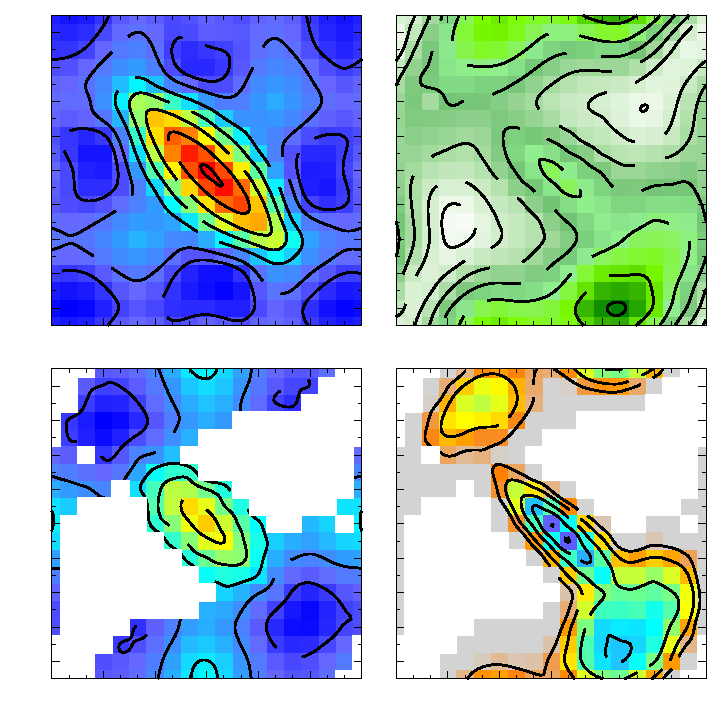
\includegraphics[width={349.00bp},height={349.00bp}]{Q1_maps}}%
    \gplfronttext
  \end{picture}%
\endgroup

  \caption[Surfaces of Q1]{Surfaces of Q1. From left to right and top to bottom: potential energy surface (CC2), dipole strength surface (DFT TPSS), PES for the VBS (EA-EOM-CC2), and PES for the DBS (EA-EOM-CC2). White points in VBS and DBS surfaces were not sampled, and gray points the DBS surface indicate that the DBS is not predicted to exist. \label{fig:Q1_maps}}
\end{figure}

Concerning the conformational potential energy surface (PES), the fixed position of the isoprene tail, distant from the quinone moiety, prevents interaction with the methoxy chains. This renders the scenario largely analogous to that of Q\textsubscript{0}. Steric hindrances would be anticipated with longer tails or alternative configurations. However, the relevance of this particular system is questionable, as crystallographic data \cite{taguchi2013conformational} indicate that the isoprene tail does not penetrate the quinone moiety's pocket. Within a protein, the orientation of the methoxy chains is dictated by the local environment, with specific configurations favoured by interactions with first-shell amino acids.\\

The interpretation of the dipole strength surface is also similar to that of Q\textsubscript{0}, with the addition of a fixed dipole originating from the isoprene group, which is oriented approximately out of the plane. This has the effect of dividing region B from Figure \ref{fig:Q0_maps} into two distinct regions for Q\textsubscript{1}, designated B and C. In region B, the local dipole of the isoprene aligns with the methoxy dipoles, resulting in a maximum dipole strength of 3.3 Debye at (160,-80). Conversely, in region C, destructive interference occurs between the local dipoles, leading to a maximum dipole strength of 2.9 Debye at (-60,160). Region A is only slightly affected, retaining a maximum dipole strength of 2.6 D at (0,0).\\

The VBS surface of Q\textsubscript{1} is more challenging to interpret due to the omitted data points. Nevertheless, the overall picture appears to remain consistent, as the qualitative effect of the rotation of the chains (acting as electron donor or acceptor) is unchanged. The range of vertical electron affinity (VEA) varies surprisingly little, with a global minimum of 1.26 eV at (0,0) and a maximum of 1.76 eV at (-120,120). It had been previously proposed that, contrary to its established spectator role, the isoprene tail might contribute to the stabilisation of the excess electron \cite{pshenichnyuk2020ionizing}. However, the results presented herein suggest that the isoprene tail does not significantly affect the VBS of Q\textsubscript{1}, at least in the conformation employed in this study.\\

Regarding the DBS surface, the impact of the isoprene tail is more pronounced. In region B, where the local dipole of the isoprene tail aligns with the methoxy dipoles, the region expands to encompass a larger area and exhibits a maximum binding energy of 9.1 meV at (80,-160). In region C, the local dipoles interfere destructively, resulting in a smaller area with a maximum binding energy of 5.0 meV at (-80,140). Region A shows a minor difference, with a maximum binding energy of 12.2 meV at (20,-20). In Figure \ref{fig:Q1_dyson}, the Dyson orbitals of the structures are shown. The variations in electron binding energy in regions B and C can be attributed to changes in the dipole moment strength. The alteration in region A, however, is likely related to a decrease in the favourable interactions between the DBS and the rest of the electronic density, as the dipole moment remains largely unchanged. Similarly to the case with Q0, it is noteworthy that structures with dipole moments below 2.5 D are predicted to be bound by EA-EOM-CC2; for example, with dihedrals of (20,20) and a dipole moment of 1.81 D, the binding energy is 2.2 meV.\\

\begin{figure}[h]
  \centering
    \begin{minipage}[b]{0.30\textwidth}
    \centering
      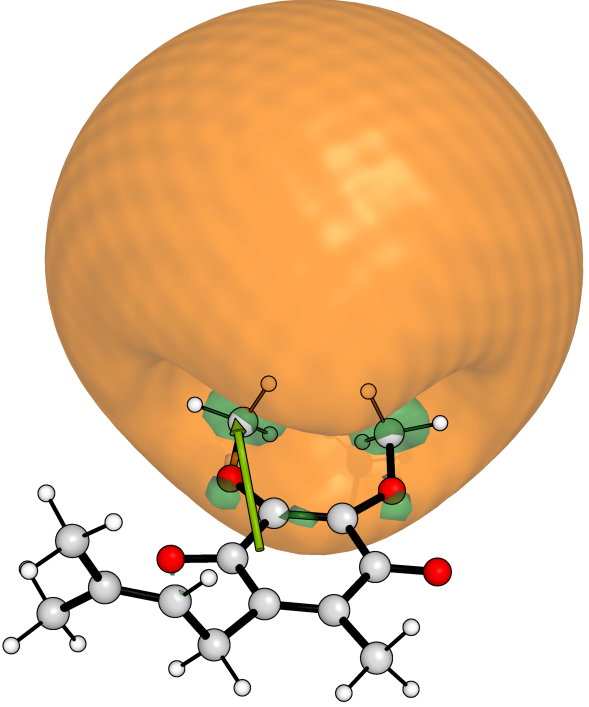
\includegraphics[width=1\textwidth]{chapters/results/image/Q1_199.png}
      \small\emph{Region A \\$(0,0)~\mu=2.6~D$ E=12.2~meV}
  \end{minipage}
  \hfill
  \begin{minipage}[b]{0.30\textwidth}
    \centering
      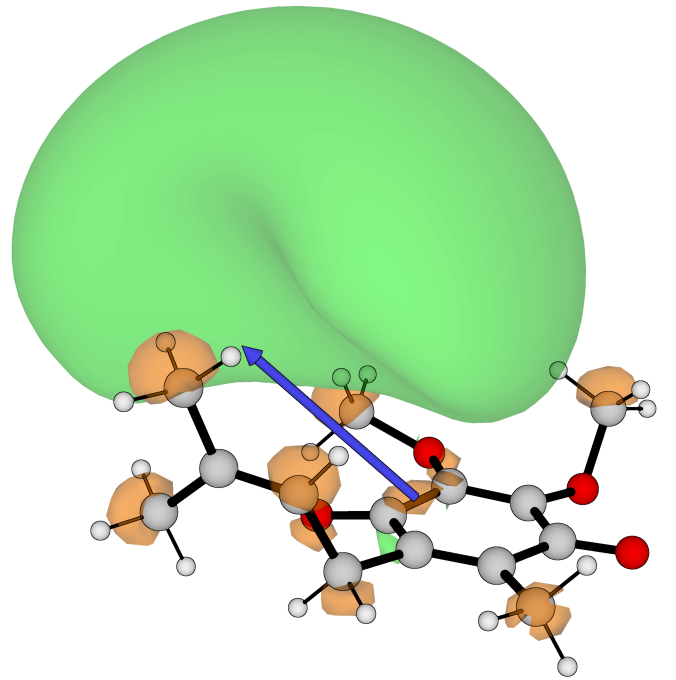
\includegraphics[width=\textwidth]{chapters/results/image/Q1_249.png}
      \small\emph{Region B \\$(160,-80)~\mu=3.3~D$, $E=9.1~meV$}
  \end{minipage}
  \hfill
  \begin{minipage}[b]{0.30\textwidth}
    \centering
    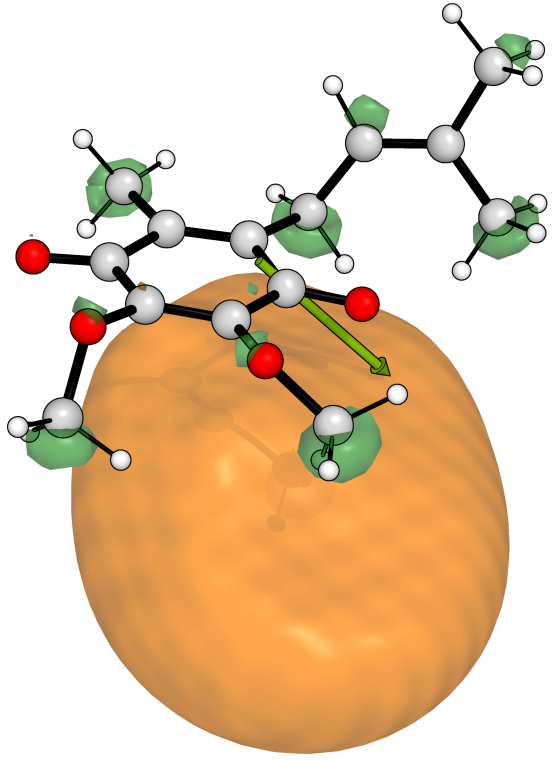
\includegraphics[width=0.9\textwidth]{chapters/results/image/Q1_112.png}
    \small\emph{Region C \\$(-60,160)~\mu=2.9~D$, $E=5.0~meV$}
  \end{minipage}
  \caption[Dyson orbitals of Q1]{Dyson orbitals of Q0 calculated with RI-EA-EOM-CC2/aug-cc-pVDZ+6s3p. The left panel shows the Dyson orbital of the strongest bound DBS from region A. The middle panel shows the Dyson orbital of the strongest bound DBS from region B. The right panel shows the Dyson orbital of the strongest bound DBS from region A. The isosurface is set to 0.005 a.u. and the dipole moment vector is shown as a blue arrow with origin at the centre of mass.}
  \label{fig:Q1_dyson}
\end{figure}

An important consideration for dipole-bound states (DBS) is the extent of correlation between their binding energy and the strength of the dipole moment that supports them. The DBS maps for Q\textsubscript{0}, Figure \ref{fig:Q0_maps}, and Q\textsubscript{1}, Figure \ref{fig:Q1_maps}, are clearly demarcated into distinct regions. Figure \ref{fig:D_vsDBS} presents a scatter plot illustrating all bound points for both Q\textsubscript{0} and Q\textsubscript{1}. This plot demonstrates that the different regions identified in the maps correspond to separate populations in the scatter plot. A correlation between dipole strength and binding energy is observed in all regions, though the degree of this correlation varies. For instance, region A, which accommodates the strongest dipoles, exhibits a nearly linear relationship between these two parameters for both quinones. This could be interepreted as the molecule acting as an ideal dipole. When comparing region A in Q\textsubscript{0} and Q\textsubscript{1}, the slope for Q\textsubscript{0} is steeper than that for Q\textsubscript{1}, indicating that variations in the chemical environment affect the interplay between the dipole moment and the binding strength.\\

Concerning the populations in regions B and C, the relationship between the dipole moment and binding energy is considerably less pronounced. This is likely because the DBS occupies a spatial region closer to the other electrons, specifically the \textpi\ system. In this system, alterations in dipole strength arise from changes in its orientation. Consequently, the displacement of the DBS that accompanies the strengthening of the dipole might result in a less favourable interaction with the remaining electronic density.
In general, the electron binding energy is only loosely correlated with the magnitude of the dipole moment that supports it. However, for analogous systems, such as region A, these two quantities become more significantly interconnected.\\

\begin{figure}[th!]
    \centering
    \small
    % GNUPLOT: LaTeX picture with Postscript
\begingroup
  \makeatletter
  \providecommand\color[2][]{%
    \GenericError{(gnuplot) \space\space\space\@spaces}{%
      Package color not loaded in conjunction with
      terminal option `colourtext'%
    }{See the gnuplot documentation for explanation.%
    }{Either use 'blacktext' in gnuplot or load the package
      color.sty in LaTeX.}%
    \renewcommand\color[2][]{}%
  }%
  \providecommand\includegraphics[2][]{%
    \GenericError{(gnuplot) \space\space\space\@spaces}{%
      Package graphicx or graphics not loaded%
    }{See the gnuplot documentation for explanation.%
    }{The gnuplot epslatex terminal needs graphicx.sty or graphics.sty.}%
    \renewcommand\includegraphics[2][]{}%
  }%
  \providecommand\rotatebox[2]{#2}%
  \@ifundefined{ifGPcolor}{%
    \newif\ifGPcolor
    \GPcolortrue
  }{}%
  \@ifundefined{ifGPblacktext}{%
    \newif\ifGPblacktext
    \GPblacktexttrue
  }{}%
  % define a \g@addto@macro without @ in the name:
  \let\gplgaddtomacro\g@addto@macro
  % define empty templates for all commands taking text:
  \gdef\gplbacktext{}%
  \gdef\gplfronttext{}%
  \makeatother
  \ifGPblacktext
    % no textcolor at all
    \def\colorrgb#1{}%
    \def\colorgray#1{}%
  \else
    % gray or color?
    \ifGPcolor
      \def\colorrgb#1{\color[rgb]{#1}}%
      \def\colorgray#1{\color[gray]{#1}}%
      \expandafter\def\csname LTw\endcsname{\color{white}}%
      \expandafter\def\csname LTb\endcsname{\color{black}}%
      \expandafter\def\csname LTa\endcsname{\color{black}}%
      \expandafter\def\csname LT0\endcsname{\color[rgb]{1,0,0}}%
      \expandafter\def\csname LT1\endcsname{\color[rgb]{0,1,0}}%
      \expandafter\def\csname LT2\endcsname{\color[rgb]{0,0,1}}%
      \expandafter\def\csname LT3\endcsname{\color[rgb]{1,0,1}}%
      \expandafter\def\csname LT4\endcsname{\color[rgb]{0,1,1}}%
      \expandafter\def\csname LT5\endcsname{\color[rgb]{1,1,0}}%
      \expandafter\def\csname LT6\endcsname{\color[rgb]{0,0,0}}%
      \expandafter\def\csname LT7\endcsname{\color[rgb]{1,0.3,0}}%
      \expandafter\def\csname LT8\endcsname{\color[rgb]{0.5,0.5,0.5}}%
    \else
      % gray
      \def\colorrgb#1{\color{black}}%
      \def\colorgray#1{\color[gray]{#1}}%
      \expandafter\def\csname LTw\endcsname{\color{white}}%
      \expandafter\def\csname LTb\endcsname{\color{black}}%
      \expandafter\def\csname LTa\endcsname{\color{black}}%
      \expandafter\def\csname LT0\endcsname{\color{black}}%
      \expandafter\def\csname LT1\endcsname{\color{black}}%
      \expandafter\def\csname LT2\endcsname{\color{black}}%
      \expandafter\def\csname LT3\endcsname{\color{black}}%
      \expandafter\def\csname LT4\endcsname{\color{black}}%
      \expandafter\def\csname LT5\endcsname{\color{black}}%
      \expandafter\def\csname LT6\endcsname{\color{black}}%
      \expandafter\def\csname LT7\endcsname{\color{black}}%
      \expandafter\def\csname LT8\endcsname{\color{black}}%
    \fi
  \fi
    \setlength{\unitlength}{0.0500bp}%
    \ifx\gptboxheight\undefined%
      \newlength{\gptboxheight}%
      \newlength{\gptboxwidth}%
      \newsavebox{\gptboxtext}%
    \fi%
    \setlength{\fboxrule}{0.5pt}%
    \setlength{\fboxsep}{1pt}%
    \definecolor{tbcol}{rgb}{1,1,1}%
\begin{picture}(6500.00,2540.00)%
    \gplgaddtomacro\gplbacktext{%
      \csname LTb\endcsname%%
      \put(420,453){\makebox(0,0)[r]{\strut{}$0$}}%
      \csname LTb\endcsname%%
      \put(420,729){\makebox(0,0)[r]{\strut{}$2$}}%
      \csname LTb\endcsname%%
      \put(420,1004){\makebox(0,0)[r]{\strut{}$4$}}%
      \csname LTb\endcsname%%
      \put(420,1280){\makebox(0,0)[r]{\strut{}$6$}}%
      \csname LTb\endcsname%%
      \put(420,1555){\makebox(0,0)[r]{\strut{}$8$}}%
      \csname LTb\endcsname%%
      \put(420,1831){\makebox(0,0)[r]{\strut{}$10$}}%
      \csname LTb\endcsname%%
      \put(420,2106){\makebox(0,0)[r]{\strut{}$12$}}%
      \csname LTb\endcsname%%
      \put(420,2382){\makebox(0,0)[r]{\strut{}$14$}}%
      \csname LTb\endcsname%%
      \put(518,277){\makebox(0,0){\strut{}$1.5$}}%
      \csname LTb\endcsname%%
      \put(1181,277){\makebox(0,0){\strut{}$2$}}%
      \csname LTb\endcsname%%
      \put(1843,277){\makebox(0,0){\strut{}$2.5$}}%
      \csname LTb\endcsname%%
      \put(2506,277){\makebox(0,0){\strut{}$3$}}%
      \csname LTb\endcsname%%
      \put(3169,277){\makebox(0,0){\strut{}$3.5$}}%
      \csname LTb\endcsname%%
      \put(810,2354){\makebox(0,0){\strut{}Q0}}%
    }%
    \gplgaddtomacro\gplfronttext{%
      \csname LTb\endcsname%%
      \put(2913,2297){\makebox(0,0)[r]{\strut{}Region A}}%
      \csname LTb\endcsname%%
      \put(2913,2122){\makebox(0,0)[r]{\strut{}Region B}}%
      \csname LTb\endcsname%%
      \put(63,1486){\rotatebox{-270.00}{\makebox(0,0){\strut{}DBS Binding Energy (meV)}}}%
      \csname LTb\endcsname%%
      \put(1976,13){\makebox(0,0){\strut{}Dipole Strength (Debye)}}%
    }%
    \gplgaddtomacro\gplbacktext{%
      \csname LTb\endcsname%%
      \put(3466,453){\makebox(0,0)[r]{\strut{}}}%
      \csname LTb\endcsname%%
      \put(3466,729){\makebox(0,0)[r]{\strut{}}}%
      \csname LTb\endcsname%%
      \put(3466,1004){\makebox(0,0)[r]{\strut{}}}%
      \csname LTb\endcsname%%
      \put(3466,1280){\makebox(0,0)[r]{\strut{}}}%
      \csname LTb\endcsname%%
      \put(3466,1555){\makebox(0,0)[r]{\strut{}}}%
      \csname LTb\endcsname%%
      \put(3466,1831){\makebox(0,0)[r]{\strut{}}}%
      \csname LTb\endcsname%%
      \put(3466,2106){\makebox(0,0)[r]{\strut{}}}%
      \csname LTb\endcsname%%
      \put(3466,2382){\makebox(0,0)[r]{\strut{}}}%
      \csname LTb\endcsname%%
      \put(3564,277){\makebox(0,0){\strut{}$1.5$}}%
      \csname LTb\endcsname%%
      \put(4226,277){\makebox(0,0){\strut{}$2$}}%
      \csname LTb\endcsname%%
      \put(4889,277){\makebox(0,0){\strut{}$2.5$}}%
      \csname LTb\endcsname%%
      \put(5552,277){\makebox(0,0){\strut{}$3$}}%
      \csname LTb\endcsname%%
      \put(6214,277){\makebox(0,0){\strut{}$3.5$}}%
      \csname LTb\endcsname%%
      \put(3855,2354){\makebox(0,0){\strut{}Q1}}%
    }%
    \gplgaddtomacro\gplfronttext{%
      \csname LTb\endcsname%%
      \put(5959,2385){\makebox(0,0)[r]{\strut{}Region A}}%
      \csname LTb\endcsname%%
      \put(5959,2209){\makebox(0,0)[r]{\strut{}Region B}}%
      \csname LTb\endcsname%%
      \put(5959,2034){\makebox(0,0)[r]{\strut{}Region C}}%
      \csname LTb\endcsname%%
      \put(5021,13){\makebox(0,0){\strut{}Dipole Strength (Debye)}}%
    }%
    \gplbacktext
    \put(0,0){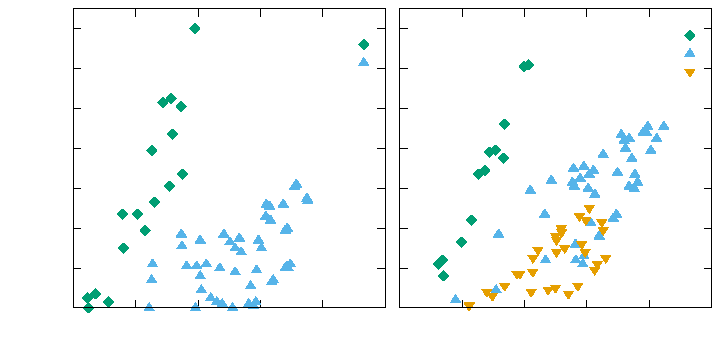
\includegraphics[width={325.00bp},height={127.00bp}]{Figs/DvsDBS}}%
    \gplfronttext
  \end{picture}%
\endgroup
 
    \caption[Q\textsubscript{0} and Q\textsubscript{1} DBS populations]{Q\textsubscript{0} and Q\textsubscript{1} DBS populations assigned to the DBS surfaces from Figures \ref{fig:Q0_maps} and \ref{fig:Q1_maps}.}
    \label{fig:D_vsDBS}
\end{figure}

\subsection{Interaction with small molecules}

Subsequent to the characterisation of the isolated quinones, the focus shifts to the interaction of their anionic states in the presence of small molecules. Recognising that chemical processes in nature do not occur in a vacuum and that environmental interactions are crucial, this work investigates these effects by considering small molecular clusters. Figure \ref{fig:scan_X} shows the interactions between Q\textsubscript{0} (region B, $\mathrm{\mu = 3.4~Debye}$, $\mathrm{EA_{DBS} = 6~meV}$), and selected molecules: methane ($\mathrm{\mu = 0~Debye}$), ammonia ($\mathrm{\mu = 1.47~Debye}$), water ($\mathrm{\mu = 1.85}$ Debye), and hydrogen fluoride ($\mathrm{\mu = 1.82~Debye}$). For these model systems, the dipole of the solvent molecule was oriented to interact either constructively or destructively with the quinone's dipole. In the case of methane, which has no dipole moment, it is shown in both cases for comparison. The intermolecular distance was systematically varied from 30 down to 4 \r{A}. The resulting effects on the VBS and DBS energies, are presented in Figure \ref{fig:scan_X}. It is important to note that none of these molecules support an anionic state on their own. The DBS of a representative Q\textsubscript{0} + water system for each of the two orientations is shown in Figure \ref{fig:Q1_dyson}.\\

\begin{figure}[th!]
    \centering
    \small
    % GNUPLOT: LaTeX picture with Postscript
\begingroup
  \makeatletter
  \providecommand\color[2][]{%
    \GenericError{(gnuplot) \space\space\space\@spaces}{%
      Package color not loaded in conjunction with
      terminal option `colourtext'%
    }{See the gnuplot documentation for explanation.%
    }{Either use 'blacktext' in gnuplot or load the package
      color.sty in LaTeX.}%
    \renewcommand\color[2][]{}%
  }%
  \providecommand\includegraphics[2][]{%
    \GenericError{(gnuplot) \space\space\space\@spaces}{%
      Package graphicx or graphics not loaded%
    }{See the gnuplot documentation for explanation.%
    }{The gnuplot epslatex terminal needs graphicx.sty or graphics.sty.}%
    \renewcommand\includegraphics[2][]{}%
  }%
  \providecommand\rotatebox[2]{#2}%
  \@ifundefined{ifGPcolor}{%
    \newif\ifGPcolor
    \GPcolortrue
  }{}%
  \@ifundefined{ifGPblacktext}{%
    \newif\ifGPblacktext
    \GPblacktexttrue
  }{}%
  % define a \g@addto@macro without @ in the name:
  \let\gplgaddtomacro\g@addto@macro
  % define empty templates for all commands taking text:
  \gdef\gplbacktext{}%
  \gdef\gplfronttext{}%
  \makeatother
  \ifGPblacktext
    % no textcolor at all
    \def\colorrgb#1{}%
    \def\colorgray#1{}%
  \else
    % gray or color?
    \ifGPcolor
      \def\colorrgb#1{\color[rgb]{#1}}%
      \def\colorgray#1{\color[gray]{#1}}%
      \expandafter\def\csname LTw\endcsname{\color{white}}%
      \expandafter\def\csname LTb\endcsname{\color{black}}%
      \expandafter\def\csname LTa\endcsname{\color{black}}%
      \expandafter\def\csname LT0\endcsname{\color[rgb]{1,0,0}}%
      \expandafter\def\csname LT1\endcsname{\color[rgb]{0,1,0}}%
      \expandafter\def\csname LT2\endcsname{\color[rgb]{0,0,1}}%
      \expandafter\def\csname LT3\endcsname{\color[rgb]{1,0,1}}%
      \expandafter\def\csname LT4\endcsname{\color[rgb]{0,1,1}}%
      \expandafter\def\csname LT5\endcsname{\color[rgb]{1,1,0}}%
      \expandafter\def\csname LT6\endcsname{\color[rgb]{0,0,0}}%
      \expandafter\def\csname LT7\endcsname{\color[rgb]{1,0.3,0}}%
      \expandafter\def\csname LT8\endcsname{\color[rgb]{0.5,0.5,0.5}}%
    \else
      % gray
      \def\colorrgb#1{\color{black}}%
      \def\colorgray#1{\color[gray]{#1}}%
      \expandafter\def\csname LTw\endcsname{\color{white}}%
      \expandafter\def\csname LTb\endcsname{\color{black}}%
      \expandafter\def\csname LTa\endcsname{\color{black}}%
      \expandafter\def\csname LT0\endcsname{\color{black}}%
      \expandafter\def\csname LT1\endcsname{\color{black}}%
      \expandafter\def\csname LT2\endcsname{\color{black}}%
      \expandafter\def\csname LT3\endcsname{\color{black}}%
      \expandafter\def\csname LT4\endcsname{\color{black}}%
      \expandafter\def\csname LT5\endcsname{\color{black}}%
      \expandafter\def\csname LT6\endcsname{\color{black}}%
      \expandafter\def\csname LT7\endcsname{\color{black}}%
      \expandafter\def\csname LT8\endcsname{\color{black}}%
    \fi
  \fi
    \setlength{\unitlength}{0.0500bp}%
    \ifx\gptboxheight\undefined%
      \newlength{\gptboxheight}%
      \newlength{\gptboxwidth}%
      \newsavebox{\gptboxtext}%
    \fi%
    \setlength{\fboxrule}{0.5pt}%
    \setlength{\fboxsep}{1pt}%
    \definecolor{tbcol}{rgb}{1,1,1}%
\begin{picture}(9060.00,9060.00)%
    \gplgaddtomacro\gplbacktext{%
      \csname LTb\endcsname%%
      \put(444,7172){\makebox(0,0)[r]{\strut{}-60}}%
      \csname LTb\endcsname%%
      \put(444,7603){\makebox(0,0)[r]{\strut{}-45}}%
      \csname LTb\endcsname%%
      \put(444,8034){\makebox(0,0)[r]{\strut{}-30}}%
      \csname LTb\endcsname%%
      \put(444,8465){\makebox(0,0)[r]{\strut{}-15}}%
      \csname LTb\endcsname%%
      \put(444,8896){\makebox(0,0)[r]{\strut{}0}}%
      \csname LTb\endcsname%%
      \put(1171,6852){\makebox(0,0){\strut{}}}%
      \csname LTb\endcsname%%
      \put(2745,6852){\makebox(0,0){\strut{}}}%
      \csname LTb\endcsname%%
      \put(4319,6852){\makebox(0,0){\strut{}}}%
      \csname LTb\endcsname%%
      \put(5892,6852){\makebox(0,0){\strut{}}}%
      \csname LTb\endcsname%%
      \put(7466,6852){\makebox(0,0){\strut{}}}%
      \csname LTb\endcsname%%
      \put(9039,6852){\makebox(0,0){\strut{}}}%
      \csname LTb\endcsname%%
      \put(4791,7229){\makebox(0,0){\strut{}DBS Opposing}}%
    }%
    \gplgaddtomacro\gplfronttext{%
    }%
    \gplgaddtomacro\gplbacktext{%
      \csname LTb\endcsname%%
      \put(444,4836){\makebox(0,0)[r]{\strut{}-2.6}}%
      \csname LTb\endcsname%%
      \put(444,5238){\makebox(0,0)[r]{\strut{}-2.4}}%
      \csname LTb\endcsname%%
      \put(444,5640){\makebox(0,0)[r]{\strut{}-2.2}}%
      \csname LTb\endcsname%%
      \put(444,6043){\makebox(0,0)[r]{\strut{}-2.0}}%
      \csname LTb\endcsname%%
      \put(444,6445){\makebox(0,0)[r]{\strut{}-1.8}}%
      \csname LTb\endcsname%%
      \put(444,6847){\makebox(0,0)[r]{\strut{}-1.6}}%
      \csname LTb\endcsname%%
      \put(1171,4660){\makebox(0,0){\strut{}}}%
      \csname LTb\endcsname%%
      \put(2745,4660){\makebox(0,0){\strut{}}}%
      \csname LTb\endcsname%%
      \put(4319,4660){\makebox(0,0){\strut{}}}%
      \csname LTb\endcsname%%
      \put(5892,4660){\makebox(0,0){\strut{}}}%
      \csname LTb\endcsname%%
      \put(7466,4660){\makebox(0,0){\strut{}}}%
      \csname LTb\endcsname%%
      \put(9039,4660){\makebox(0,0){\strut{}}}%
      \csname LTb\endcsname%%
      \put(4791,5037){\makebox(0,0){\strut{}VBS Opposing}}%
    }%
    \gplgaddtomacro\gplfronttext{%
    }%
    \gplgaddtomacro\gplbacktext{%
      \csname LTb\endcsname%%
      \put(444,2644){\makebox(0,0)[r]{\strut{}-80}}%
      \csname LTb\endcsname%%
      \put(444,3117){\makebox(0,0)[r]{\strut{}-60}}%
      \csname LTb\endcsname%%
      \put(444,3590){\makebox(0,0)[r]{\strut{}-40}}%
      \csname LTb\endcsname%%
      \put(444,4063){\makebox(0,0)[r]{\strut{}-20}}%
      \csname LTb\endcsname%%
      \put(444,4537){\makebox(0,0)[r]{\strut{}0}}%
      \csname LTb\endcsname%%
      \put(1171,2468){\makebox(0,0){\strut{}}}%
      \csname LTb\endcsname%%
      \put(2745,2468){\makebox(0,0){\strut{}}}%
      \csname LTb\endcsname%%
      \put(4319,2468){\makebox(0,0){\strut{}}}%
      \csname LTb\endcsname%%
      \put(5892,2468){\makebox(0,0){\strut{}}}%
      \csname LTb\endcsname%%
      \put(7466,2468){\makebox(0,0){\strut{}}}%
      \csname LTb\endcsname%%
      \put(9039,2468){\makebox(0,0){\strut{}}}%
      \csname LTb\endcsname%%
      \put(4791,2845){\makebox(0,0){\strut{}DBS Parallel}}%
    }%
    \gplgaddtomacro\gplfronttext{%
    }%
    \gplgaddtomacro\gplbacktext{%
      \csname LTb\endcsname%%
      \put(444,452){\makebox(0,0)[r]{\strut{}-2.0}}%
      \csname LTb\endcsname%%
      \put(444,1122){\makebox(0,0)[r]{\strut{}-1.8}}%
      \csname LTb\endcsname%%
      \put(444,1792){\makebox(0,0)[r]{\strut{}-1.6}}%
      \csname LTb\endcsname%%
      \put(444,2463){\makebox(0,0)[r]{\strut{}-1.4}}%
      \csname LTb\endcsname%%
      \put(1171,276){\makebox(0,0){\strut{}$5$}}%
      \csname LTb\endcsname%%
      \put(2745,276){\makebox(0,0){\strut{}$10$}}%
      \csname LTb\endcsname%%
      \put(4319,276){\makebox(0,0){\strut{}$15$}}%
      \csname LTb\endcsname%%
      \put(5892,276){\makebox(0,0){\strut{}$20$}}%
      \csname LTb\endcsname%%
      \put(7466,276){\makebox(0,0){\strut{}$25$}}%
      \csname LTb\endcsname%%
      \put(9039,276){\makebox(0,0){\strut{}$30$}}%
      \csname LTb\endcsname%%
      \put(4791,653){\makebox(0,0){\strut{}VBS Parallel}}%
    }%
    \gplgaddtomacro\gplfronttext{%
      \csname LTb\endcsname%%
      \put(4791,12){\makebox(0,0){\strut{}Distance (\AA)}}%
    }%
    \gplbacktext
    \put(0,0){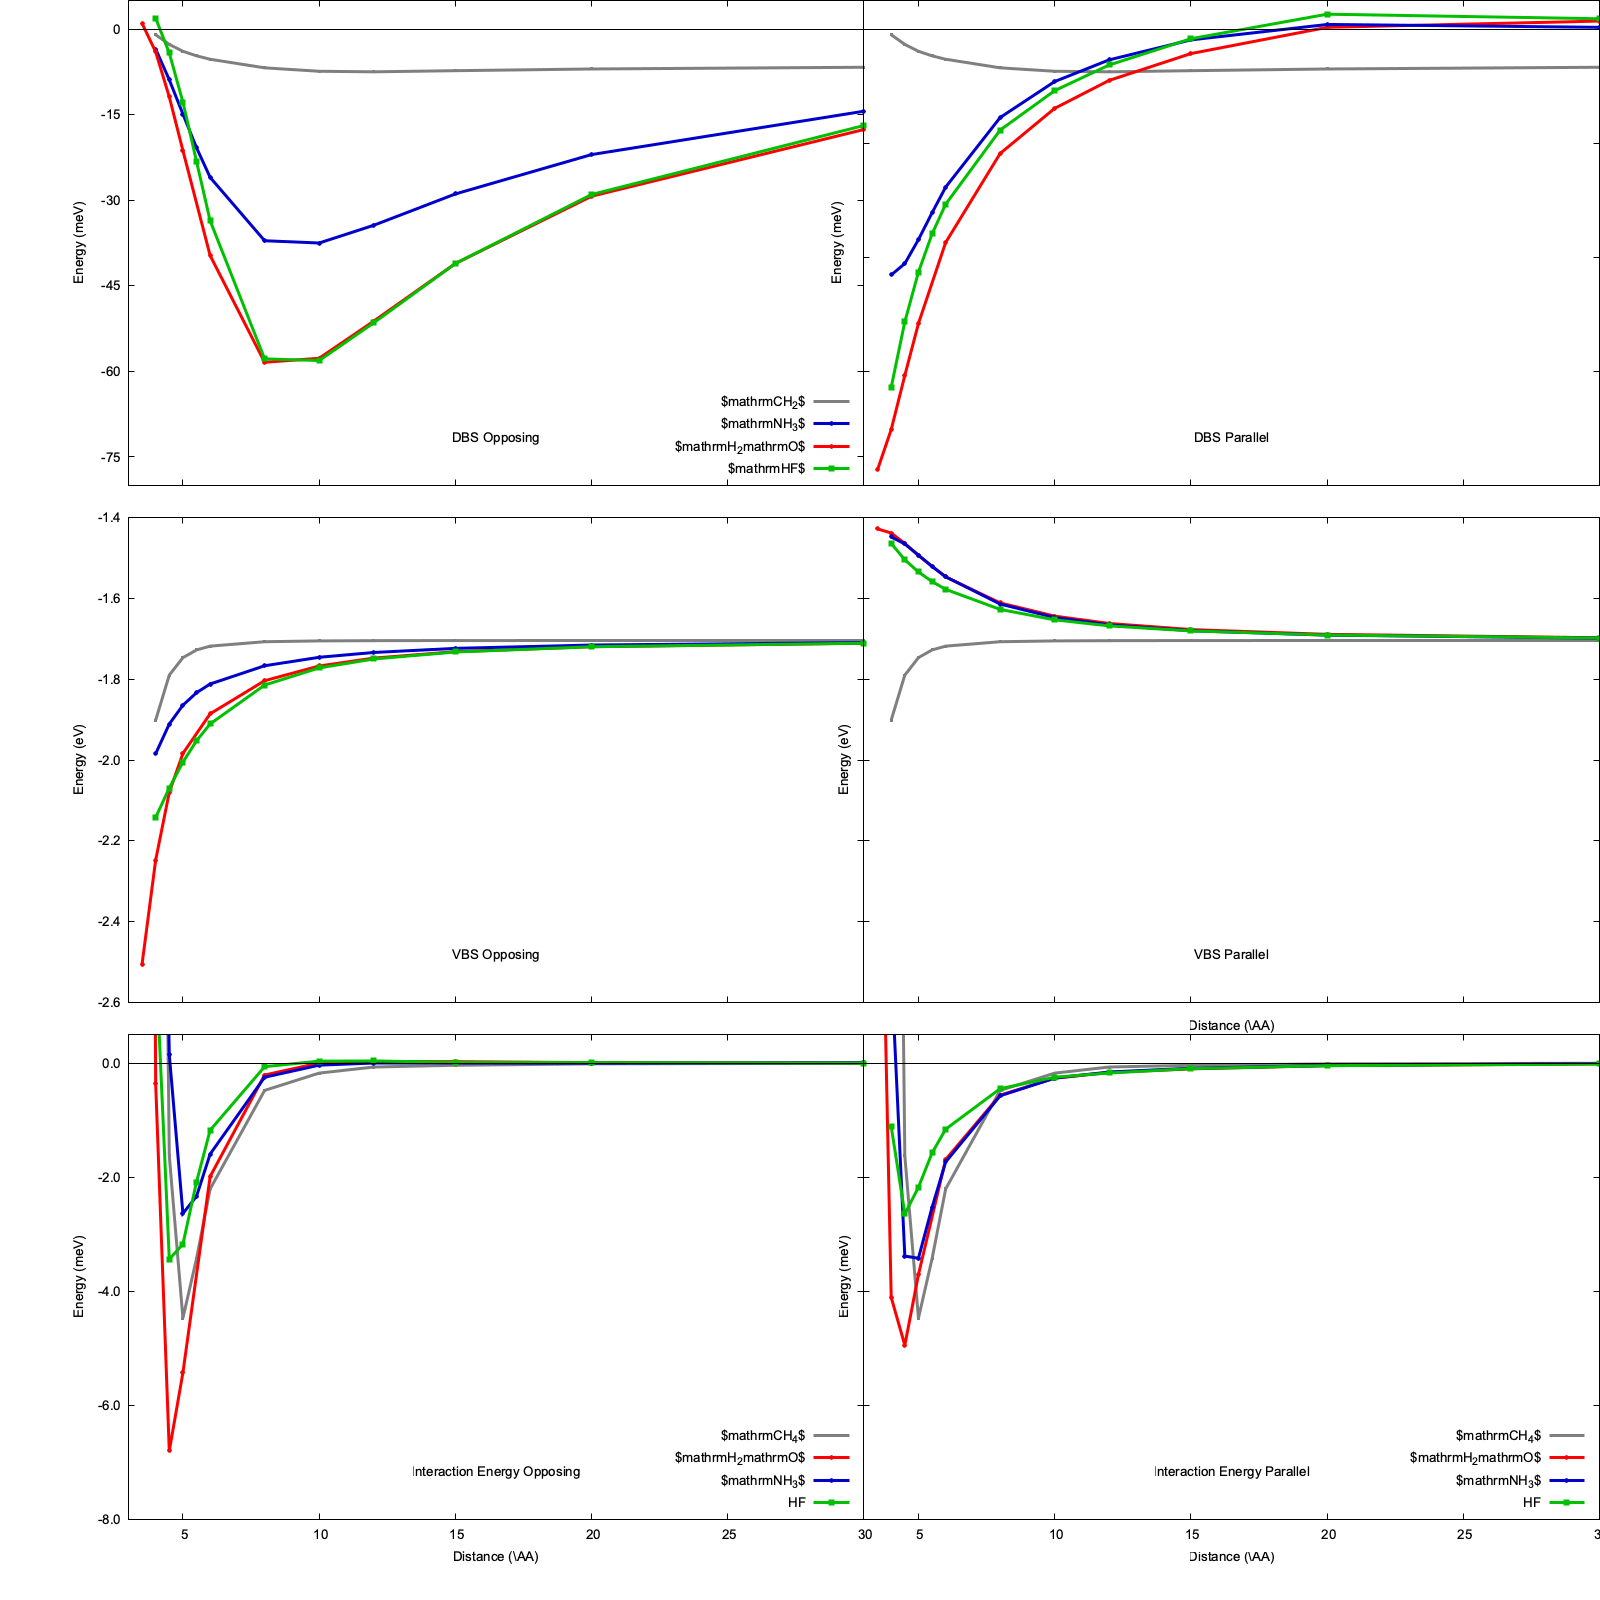
\includegraphics[width={453.00bp},height={453.00bp}]{chapters/results/image/scan_all}}%
    \gplfronttext
  \end{picture}%
\endgroup

    %% GNUPLOT: LaTeX picture with Postscript
\begingroup
  \makeatletter
  \providecommand\color[2][]{%
    \GenericError{(gnuplot) \space\space\space\@spaces}{%
      Package color not loaded in conjunction with
      terminal option `colourtext'%
    }{See the gnuplot documentation for explanation.%
    }{Either use 'blacktext' in gnuplot or load the package
      color.sty in LaTeX.}%
    \renewcommand\color[2][]{}%
  }%
  \providecommand\includegraphics[2][]{%
    \GenericError{(gnuplot) \space\space\space\@spaces}{%
      Package graphicx or graphics not loaded%
    }{See the gnuplot documentation for explanation.%
    }{The gnuplot epslatex terminal needs graphicx.sty or graphics.sty.}%
    \renewcommand\includegraphics[2][]{}%
  }%
  \providecommand\rotatebox[2]{#2}%
  \@ifundefined{ifGPcolor}{%
    \newif\ifGPcolor
    \GPcolortrue
  }{}%
  \@ifundefined{ifGPblacktext}{%
    \newif\ifGPblacktext
    \GPblacktexttrue
  }{}%
  % define a \g@addto@macro without @ in the name:
  \let\gplgaddtomacro\g@addto@macro
  % define empty templates for all commands taking text:
  \gdef\gplbacktext{}%
  \gdef\gplfronttext{}%
  \makeatother
  \ifGPblacktext
    % no textcolor at all
    \def\colorrgb#1{}%
    \def\colorgray#1{}%
  \else
    % gray or color?
    \ifGPcolor
      \def\colorrgb#1{\color[rgb]{#1}}%
      \def\colorgray#1{\color[gray]{#1}}%
      \expandafter\def\csname LTw\endcsname{\color{white}}%
      \expandafter\def\csname LTb\endcsname{\color{black}}%
      \expandafter\def\csname LTa\endcsname{\color{black}}%
      \expandafter\def\csname LT0\endcsname{\color[rgb]{1,0,0}}%
      \expandafter\def\csname LT1\endcsname{\color[rgb]{0,1,0}}%
      \expandafter\def\csname LT2\endcsname{\color[rgb]{0,0,1}}%
      \expandafter\def\csname LT3\endcsname{\color[rgb]{1,0,1}}%
      \expandafter\def\csname LT4\endcsname{\color[rgb]{0,1,1}}%
      \expandafter\def\csname LT5\endcsname{\color[rgb]{1,1,0}}%
      \expandafter\def\csname LT6\endcsname{\color[rgb]{0,0,0}}%
      \expandafter\def\csname LT7\endcsname{\color[rgb]{1,0.3,0}}%
      \expandafter\def\csname LT8\endcsname{\color[rgb]{0.5,0.5,0.5}}%
    \else
      % gray
      \def\colorrgb#1{\color{black}}%
      \def\colorgray#1{\color[gray]{#1}}%
      \expandafter\def\csname LTw\endcsname{\color{white}}%
      \expandafter\def\csname LTb\endcsname{\color{black}}%
      \expandafter\def\csname LTa\endcsname{\color{black}}%
      \expandafter\def\csname LT0\endcsname{\color{black}}%
      \expandafter\def\csname LT1\endcsname{\color{black}}%
      \expandafter\def\csname LT2\endcsname{\color{black}}%
      \expandafter\def\csname LT3\endcsname{\color{black}}%
      \expandafter\def\csname LT4\endcsname{\color{black}}%
      \expandafter\def\csname LT5\endcsname{\color{black}}%
      \expandafter\def\csname LT6\endcsname{\color{black}}%
      \expandafter\def\csname LT7\endcsname{\color{black}}%
      \expandafter\def\csname LT8\endcsname{\color{black}}%
    \fi
  \fi
    \setlength{\unitlength}{0.0500bp}%
    \ifx\gptboxheight\undefined%
      \newlength{\gptboxheight}%
      \newlength{\gptboxwidth}%
      \newsavebox{\gptboxtext}%
    \fi%
    \setlength{\fboxrule}{0.5pt}%
    \setlength{\fboxsep}{1pt}%
    \definecolor{tbcol}{rgb}{1,1,1}%
\begin{picture}(6980.00,3200.00)%
    \gplgaddtomacro\gplbacktext{%
      \csname LTb\endcsname%%
      \put(598,1728){\makebox(0,0)[r]{\strut{}-60}}%
      \csname LTb\endcsname%%
      \put(598,2048){\makebox(0,0)[r]{\strut{}-45}}%
      \csname LTb\endcsname%%
      \put(598,2369){\makebox(0,0)[r]{\strut{}-30}}%
      \csname LTb\endcsname%%
      \put(598,2689){\makebox(0,0)[r]{\strut{}-15}}%
      \csname LTb\endcsname%%
      \put(598,3009){\makebox(0,0)[r]{\strut{}0}}%
      \csname LTb\endcsname%%
      \put(1149,1445){\makebox(0,0){\strut{}}}%
      \csname LTb\endcsname%%
      \put(2283,1445){\makebox(0,0){\strut{}}}%
      \csname LTb\endcsname%%
      \put(3418,1445){\makebox(0,0){\strut{}}}%
      \csname LTb\endcsname%%
      \put(4552,1445){\makebox(0,0){\strut{}}}%
      \csname LTb\endcsname%%
      \put(5686,1445){\makebox(0,0){\strut{}}}%
      \csname LTb\endcsname%%
      \put(6820,1445){\makebox(0,0){\strut{}}}%
      \csname LTb\endcsname%%
      \put(3758,1771){\makebox(0,0){\strut{}DBS Opposing}}%
    }%
    \gplgaddtomacro\gplfronttext{%
      \csname LTb\endcsname%%
      \put(45,2369){\rotatebox{-270.00}{\makebox(0,0){\strut{}Energy (meV)}}}%
    }%
    \gplgaddtomacro\gplbacktext{%
      \csname LTb\endcsname%%
      \put(598,31){\makebox(0,0)[r]{\strut{}-2.6}}%
      \csname LTb\endcsname%%
      \put(598,330){\makebox(0,0)[r]{\strut{}-2.4}}%
      \csname LTb\endcsname%%
      \put(598,629){\makebox(0,0)[r]{\strut{}-2.2}}%
      \csname LTb\endcsname%%
      \put(598,928){\makebox(0,0)[r]{\strut{}-2.0}}%
      \csname LTb\endcsname%%
      \put(598,1227){\makebox(0,0)[r]{\strut{}-1.8}}%
      \csname LTb\endcsname%%
      \put(598,1526){\makebox(0,0)[r]{\strut{}-1.6}}%
      \csname LTb\endcsname%%
      \put(3758,181){\makebox(0,0){\strut{}VBS Opposing}}%
    }%
    \gplgaddtomacro\gplfronttext{%
      \csname LTb\endcsname%%
      \put(45,779){\rotatebox{-270.00}{\makebox(0,0){\strut{}Energy (eV)}}}%
    }%
    \gplbacktext
    \put(0,0){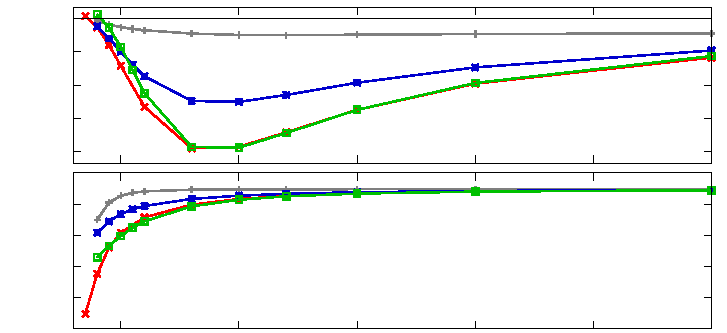
\includegraphics[width={349.00bp},height={160.00bp}]{scan_H}}%
    \gplfronttext
  \end{picture}%
\endgroup

    %% GNUPLOT: LaTeX picture with Postscript
\begingroup
  \makeatletter
  \providecommand\color[2][]{%
    \GenericError{(gnuplot) \space\space\space\@spaces}{%
      Package color not loaded in conjunction with
      terminal option `colourtext'%
    }{See the gnuplot documentation for explanation.%
    }{Either use 'blacktext' in gnuplot or load the package
      color.sty in LaTeX.}%
    \renewcommand\color[2][]{}%
  }%
  \providecommand\includegraphics[2][]{%
    \GenericError{(gnuplot) \space\space\space\@spaces}{%
      Package graphicx or graphics not loaded%
    }{See the gnuplot documentation for explanation.%
    }{The gnuplot epslatex terminal needs graphicx.sty or graphics.sty.}%
    \renewcommand\includegraphics[2][]{}%
  }%
  \providecommand\rotatebox[2]{#2}%
  \@ifundefined{ifGPcolor}{%
    \newif\ifGPcolor
    \GPcolortrue
  }{}%
  \@ifundefined{ifGPblacktext}{%
    \newif\ifGPblacktext
    \GPblacktexttrue
  }{}%
  % define a \g@addto@macro without @ in the name:
  \let\gplgaddtomacro\g@addto@macro
  % define empty templates for all commands taking text:
  \gdef\gplbacktext{}%
  \gdef\gplfronttext{}%
  \makeatother
  \ifGPblacktext
    % no textcolor at all
    \def\colorrgb#1{}%
    \def\colorgray#1{}%
  \else
    % gray or color?
    \ifGPcolor
      \def\colorrgb#1{\color[rgb]{#1}}%
      \def\colorgray#1{\color[gray]{#1}}%
      \expandafter\def\csname LTw\endcsname{\color{white}}%
      \expandafter\def\csname LTb\endcsname{\color{black}}%
      \expandafter\def\csname LTa\endcsname{\color{black}}%
      \expandafter\def\csname LT0\endcsname{\color[rgb]{1,0,0}}%
      \expandafter\def\csname LT1\endcsname{\color[rgb]{0,1,0}}%
      \expandafter\def\csname LT2\endcsname{\color[rgb]{0,0,1}}%
      \expandafter\def\csname LT3\endcsname{\color[rgb]{1,0,1}}%
      \expandafter\def\csname LT4\endcsname{\color[rgb]{0,1,1}}%
      \expandafter\def\csname LT5\endcsname{\color[rgb]{1,1,0}}%
      \expandafter\def\csname LT6\endcsname{\color[rgb]{0,0,0}}%
      \expandafter\def\csname LT7\endcsname{\color[rgb]{1,0.3,0}}%
      \expandafter\def\csname LT8\endcsname{\color[rgb]{0.5,0.5,0.5}}%
    \else
      % gray
      \def\colorrgb#1{\color{black}}%
      \def\colorgray#1{\color[gray]{#1}}%
      \expandafter\def\csname LTw\endcsname{\color{white}}%
      \expandafter\def\csname LTb\endcsname{\color{black}}%
      \expandafter\def\csname LTa\endcsname{\color{black}}%
      \expandafter\def\csname LT0\endcsname{\color{black}}%
      \expandafter\def\csname LT1\endcsname{\color{black}}%
      \expandafter\def\csname LT2\endcsname{\color{black}}%
      \expandafter\def\csname LT3\endcsname{\color{black}}%
      \expandafter\def\csname LT4\endcsname{\color{black}}%
      \expandafter\def\csname LT5\endcsname{\color{black}}%
      \expandafter\def\csname LT6\endcsname{\color{black}}%
      \expandafter\def\csname LT7\endcsname{\color{black}}%
      \expandafter\def\csname LT8\endcsname{\color{black}}%
    \fi
  \fi
    \setlength{\unitlength}{0.0500bp}%
    \ifx\gptboxheight\undefined%
      \newlength{\gptboxheight}%
      \newlength{\gptboxwidth}%
      \newsavebox{\gptboxtext}%
    \fi%
    \setlength{\fboxrule}{0.5pt}%
    \setlength{\fboxsep}{1pt}%
    \definecolor{tbcol}{rgb}{1,1,1}%
\begin{picture}(6980.00,3480.00)%
    \gplgaddtomacro\gplbacktext{%
      \csname LTb\endcsname%%
      \put(598,2006){\makebox(0,0)[r]{\strut{}-80}}%
      \csname LTb\endcsname%%
      \put(598,2332){\makebox(0,0)[r]{\strut{}-60}}%
      \csname LTb\endcsname%%
      \put(598,2658){\makebox(0,0)[r]{\strut{}-40}}%
      \csname LTb\endcsname%%
      \put(598,2983){\makebox(0,0)[r]{\strut{}-20}}%
      \csname LTb\endcsname%%
      \put(598,3309){\makebox(0,0)[r]{\strut{}0}}%
      \csname LTb\endcsname%%
      \put(1149,1830){\makebox(0,0){\strut{}}}%
      \csname LTb\endcsname%%
      \put(2283,1830){\makebox(0,0){\strut{}}}%
      \csname LTb\endcsname%%
      \put(3418,1830){\makebox(0,0){\strut{}}}%
      \csname LTb\endcsname%%
      \put(4552,1830){\makebox(0,0){\strut{}}}%
      \csname LTb\endcsname%%
      \put(5686,1830){\makebox(0,0){\strut{}}}%
      \csname LTb\endcsname%%
      \put(6820,1830){\makebox(0,0){\strut{}}}%
      \csname LTb\endcsname%%
      \put(3758,2145){\makebox(0,0){\strut{}DBS Parallel}}%
    }%
    \gplgaddtomacro\gplfronttext{%
      \csname LTb\endcsname%%
      \put(45,2698){\rotatebox{-270.00}{\makebox(0,0){\strut{}Energy (meV)}}}%
    }%
    \gplgaddtomacro\gplbacktext{%
      \csname LTb\endcsname%%
      \put(598,519){\makebox(0,0)[r]{\strut{}-2.0}}%
      \csname LTb\endcsname%%
      \put(598,980){\makebox(0,0)[r]{\strut{}-1.8}}%
      \csname LTb\endcsname%%
      \put(598,1441){\makebox(0,0)[r]{\strut{}-1.6}}%
      \csname LTb\endcsname%%
      \put(598,1902){\makebox(0,0)[r]{\strut{}-1.4}}%
      \csname LTb\endcsname%%
      \put(1149,343){\makebox(0,0){\strut{}$5$}}%
      \csname LTb\endcsname%%
      \put(2283,343){\makebox(0,0){\strut{}$10$}}%
      \csname LTb\endcsname%%
      \put(3418,343){\makebox(0,0){\strut{}$15$}}%
      \csname LTb\endcsname%%
      \put(4552,343){\makebox(0,0){\strut{}$20$}}%
      \csname LTb\endcsname%%
      \put(5686,343){\makebox(0,0){\strut{}$25$}}%
      \csname LTb\endcsname%%
      \put(6820,343){\makebox(0,0){\strut{}$30$}}%
      \csname LTb\endcsname%%
      \put(3758,657){\makebox(0,0){\strut{}VBS Parallel}}%
    }%
    \gplgaddtomacro\gplfronttext{%
      \csname LTb\endcsname%%
      \put(45,1210){\rotatebox{-270.00}{\makebox(0,0){\strut{}Energy (eV)}}}%
      \csname LTb\endcsname%%
      \put(3758,79){\makebox(0,0){\strut{}Distance (\AA)}}%
    }%
    \gplbacktext
    \put(0,0){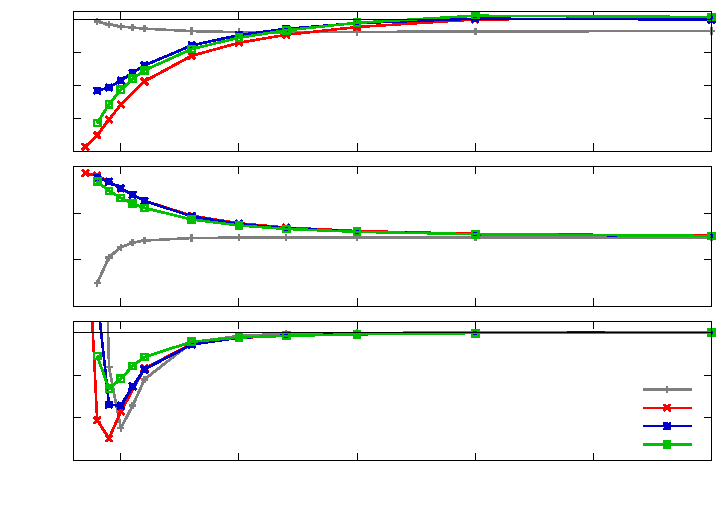
\includegraphics[width={349.00bp},height={174.00bp}]{scan_X}}%
    \gplfronttext
  \end{picture}%
\endgroup

    %figsize is set in image/test.gp 
    \caption[Q\textsubscript{0} interaction with small molecules]{Q\textsubscript{0} interaction with small molecules. From top to bottom: DBS with opposing dipoles, VBS with opposing dipoles, DBS with aligned dipoles, and VBS with aligned dipoles.}
    \label{fig:scan_X}
\end{figure}

Considering the DBS, when the solvent and quinone dipoles are opposed, polar molecules induce a wide well with a minimum at around 8 \r{A}. The electron binding energy of the DBS reaches 60 meV with both water and HF, and 37 meV with ammonia. This represents a more than tenfold increase compared to the 5.4 meV binding energy of the isolated quinone. Stabilisation by methane is considerably weaker, as it arises solely from dispersion forces. The similarity between the water and HF interaction curves is noteworthy; they overlap almost perfectly across most of the separation range. This congruence is attributed to their comparable dipole moments (1.85 D for water; 1.82 D for HF). At large separations, the specific electronic structures of these solvent molecules are less influential, and the DBS primarily experiences the effect of their dipole moments. The interaction with ammonia is weaker due to its smaller dipole moment of 1.47 D. This scenario is characteristic of a solvated electron within a `cavity' \cite{jordan2003theory,herbert2019structure}. At an intermolecular distance of approximately 4 \r{A}, the interaction becomes repulsive for all molecules studied due to steric interactions, causing the DBS to become unbound due to steric hindrance.\\

Conversely, with parallel dipole orientations, polar molecules exhibit repulsion at large distances. This is attributable to the negative end of the solvent dipole destabilising the DBS. At shorter ranges, however, the local dipoles combine constructively, thereby stabilising the binding energy. For water, which possesses the largest dipole moment, the DBS attains an electron binding energy of 80 meV, with the total system dipole moment being 6.1 Debye. Such configurations have recently been observed in photoelectron spectroscopy experiments \cite{clarke2025role} and are thought to play an important role in the transfer of a VBS to a solvated electron.\\

\begin{figure}[h]
  \centering
    \begin{minipage}[b]{0.3\textwidth}
    \centering
      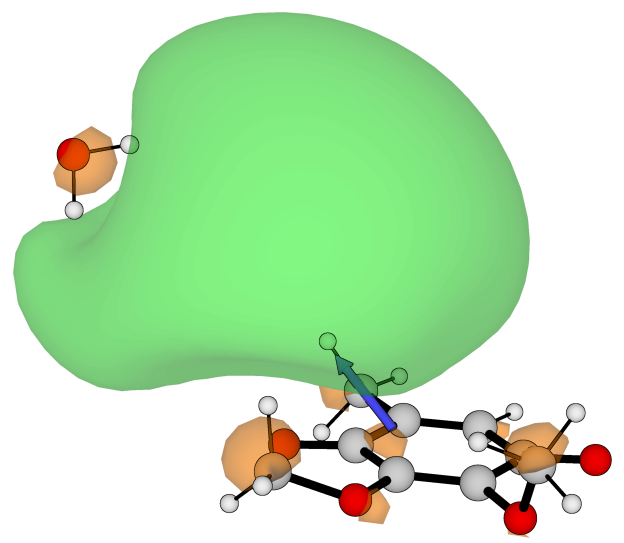
\includegraphics[width=0.9\textwidth]{chapters/results/image/Q0_H2O_H.png}
      %\small\emph{Region A \\$(0,0)~\mu=2.6~D$ E=12.2~meV}
  \end{minipage}
  \hfill
  \begin{minipage}[b]{0.3\textwidth}
    \centering
    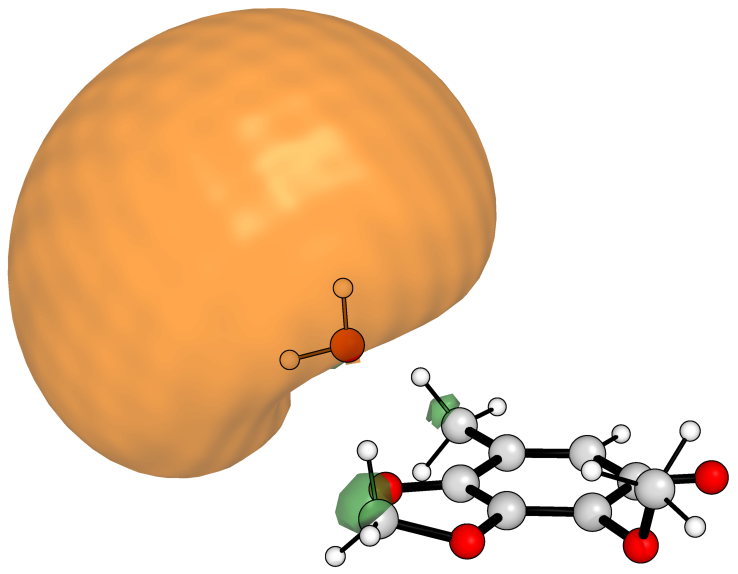
\includegraphics[width=1\textwidth]{chapters/results/image/Q0_H2O_O.png}
    %\small\emph{Region C \\$(-60,160)~\mu=2.9~D$, $E=5.0~meV$}
  \end{minipage}
  \hfill
  \begin{minipage}[b]{0.3\textwidth}
    \centering
    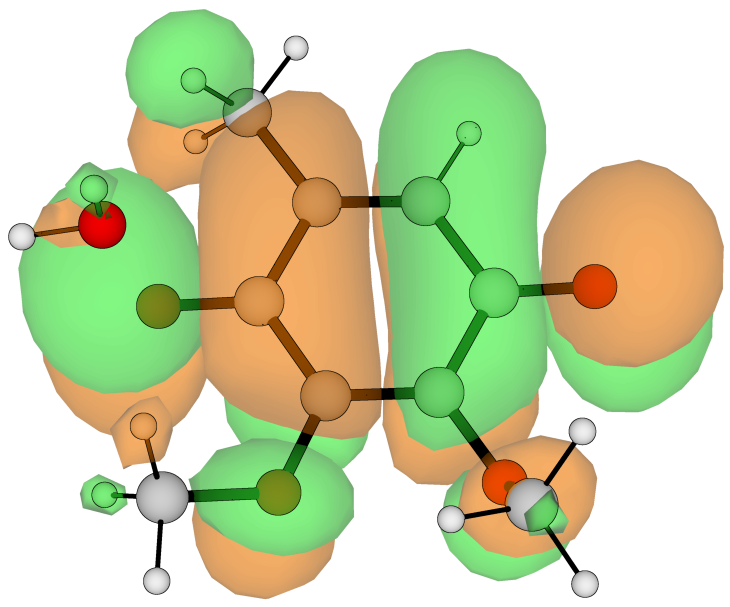
\includegraphics[width=0.9\textwidth]{chapters/results/image/Q0_H2O_VBS.png}
    %\small\emph{Region C \\$(-60,160)~\mu=2.9~D$, $E=5.0~meV$}
  \end{minipage}
  \caption[Dyson orbitals of Q0+water]{Dyson orbitals of Q0 + water calculated with RI-EA-EOM-CC2/aug-cc-pVDZ+6s3p. Left, system where the dipoles are pointing in opposite directions at an intermolecular distance of 8 \r{A}. Middle: dipoles aligned at an intermolecular distance of 4 \r{A}. Right: VBS of Q0 and a water molecule at 4 \r{A}. The isosurface is set to 0.01 a.u. and the dipole moment vector is shown as a blue arrow with origin at the centre of mass.}
  \label{fig:Q0_H2O_dyson}
\end{figure}

The interaction also significantly affects the VBS. When the dipoles are opposed, \textit{i.e.}, the positive end of the solvent dipole is oriented towards the excess electronic charge of the quinone, the VBS is strongly stabilised at short intermolecular distances. With water, the VBS achieves a VEA of 2.5 eV, an increase of over 0.8 eV compared to the isolated quinone. A similar effect is observed for HF, yielding a VEA of 2.5 eV, while the stabilisation is less pronounced for ammonia and methane. A comparison of the influence of surrounding molecules on the VBS with that of methoxy chain rotation, as discussed in section \ref{sec:Q0_maps}, reveals that intermolecular interactions can be considerably more influential. The protein environment has probably a larger effect on the CoQ EA than the orientation adopted by the methoxy chains.\\

If the dipoles are aligned, the negative end of the solvent dipole interacts with the VBS and is destabilised. A similar and unfavourable trend is observed for the three polar molecules. At an intermolecular distance of 4 \r{A}, the VEA decreases to approximately 1.4 eV. The destabilisation arises from the negative end of the solvent dipole repelling the excess electron density of the quinone.\\

Regarding the total interaction energy of the neutral system, it is important to note that the interaction with the solvent molecules is always attractive. Additionally the dipole-dipole interaction is not the main driver of the energy curve, as it can be observed how for the case of water of HF, opposing dipoles lead to a deeper well than aligned dipoles. This observation can be rationalised by a similar argument to that of the VBS, which is a \textpi \textsuperscript{*} state. The interactions of the dipole of the solvent molecule with the \textpi system of the quinone is stronger than that of the dipole-dipole energy.
%\subsection{Effect of Nearby Amionacids}


%%%%%%%%%%%%%%%%%%%%%%%%%%%%%%%%%%%%%%%%%%%%%%%%%%
% Keep the following \cleardoublepage at the end of this file, 
% otherwise \includeonly includes empty pages.
\cleardoublepage

% vim: tw=70 nocindent expandtab foldmethod=marker foldmarker={{{}{,}{}}}
% !TeX root = ../../thesis.tex
\chapter{Conclusion and Outlook}\label{ch:conclusion}
This thesis presents a theoretical investigation of anionic states of ubiquinone, which supports both a dipole-bound state and valence-bound states, primarily through equation-of-motion coupled-cluster (EOM-CC) techniques. The principal objectives included benchmarking EOM-CC2-based approaches, assessing basis set considerations for DBSs, implementating of Dyson orbitals for EOM-CC2, and applying these methods to ubiquinone (CoQ) analogues, Q\textsubscript{0} and Q\textsubscript{1}.\\

Scrutiny of basis set dependence for EA-EOM-CC2 revealed that, although larger cardinality sets (e.g.\ aug-cc-pVTZ) are often beneficial, the inclusion sufficiently diffuse functions is critical for describing the spatial extension of DBS orbitals. In general CC2 tends to overbind these states when compared to CCSD.\\

For VBSs, EA-EOM-CC2 was benchmarked against known quinones, showing that spin-component scaling (SCS) notably improves accuracy relative to uncorrected CC2. EA-EOM-CC2-SCS tends to slightly underbind the VBS states. However, unscaled CC2 has a consistent error and is able to recover the trends. The diffuse functions integral to DBSs had minimal impact on VBS energies, as they are much more localized in space.\\

A methodological advance was the implementation of EOM-CC2 Dyson orbitals. Their quality was assessed by comparing them to EOM-CCSD Dyson orbitals and HF orbitals in the calculation of photodetachment cross-sections. Validating EOM-CC2 Dyson orbitals as a resource-efficient alternative to EOM-CCSD.\\

Investigations of Q\textsubscript{0} revealed the interplay between methoxy chain conformations and the resulting potential energy, dipole moment, VBS, and DBS surfaces. Five minima were detected on the neutral PES, with methoxy group orientations dictating the dipole moment and hence affecting DBS energies.\\

Extending to Q\textsubscript{1}, the attached isoprene tail altered the overall molecular dipole to create changes in DBS binding, with constructive dipolar alignment enhancing DBS stability and destructive alignment reducing it. The VBS of Q\textsubscript{1} was not particularly sensitive to the isoprene tail's presence.  Different modes of DBS stabilization where observed, depending on their interaction with the rest of that electronic density. Within each mode, or region, the DBS binding strength seems to be correlated strongly with dipole magnitude.\\

Preliminary explorations of interactions between Q\textsubscript{0} and small molecules (methane, ammonia, water, HF) underscored the sensitivity of both VBSs and DBSs to the local environment. This outcome emphasises the importance of considering environmental effects, which is essential to model states in condensed-phase or biological settings.\\

Overall, this thesis advances the understanding of non-valence anionic states and the computational techniques applied to them. The benchmarking of EA-EOM-CC2 furnishes guidelines for those seeking cost-effective yet reliable estimates of electron affinities, DBSs, and VBSs, while confirming the utility of EOM-CC2 Dyson orbitals in photodetachment studies. The exploration of ubiquinone anion states underscores how molecular conformation and local electrostatic factors govern the stability and character of both VBSs and DBSs. The observation of DBSs supported by smaller dipole moments challenges common assumptions, highlighting the relevance of dispersion-type interactions in NVSs.\\

From a pedagogical perspective, this work comprehensively spans multiple facets of theoretical chemistry and computational modelling. Starting from the bottom with a derivation of an algebraic expression for EOM-CC2 Dyson orbitals, progresses to their implementation in commercial quantum-chemistry software, and culminates in their application to a sizeable \textit{(bio)}chemical challenge: the anionic states of ubiquinone.\\

Despite these contributions, several directions for further work remain:
\begin{itemize}
    \item \textbf{Advanced Solvation Models:} Though small-molecule interactions were considered, explicit solvation or hybrid QM/MM simulations could quantitatively characterise environmental influence on VBS and DBS formation in solution or protein settings. Other techniques that could be utilised is electrostatic embedding.
    \item \textbf{Dynamic Effects:} For larger systems that include more solvating molecules, introducing molecular dynamics simulations to account for structural fluctuations would offer insights into anion state energies and interconversions under realistic conditions.
    \item \textbf{Relating to Experimental Observables:} Future efforts could concentrate on predicting and interpreting experimental data, such as electron transmission, photoelectron angular distributions, or connecting VBS/DBS energies to redox properties in electrochemical or biochemical contexts. Specificaly, one could compute the nonadiabatic couplings between a potential electron donor state and the VBS and
\end{itemize}
    
In summary, this thesis offers a thorough computational analysis of non-valence anions, supplies methodological insights, and delivers a closer characterisation of ubiquinone anion states. These outcomes pave the way for further studies of the complex physics and chemistry associated with such species in larger or more intricate biological frameworks.


%%%%%%%%%%%%%%%%%%%%%%%%%%%%%%%%%%%%%%%%%%%%%%%%%%
% Keep the following \cleardoublepage at the end of this file, 
% otherwise \includeonly includes empty pages.
\cleardoublepage

% vim: tw=70 nocindent expandtab foldmethod=marker foldmarker={{{}{,}{}}}


\printbibliography

%\bibliographystyle{naturemag}
%\phantomsection
%\addcontentsline{toc}{chapter}{Bibliography}
%\bibliography{allpapers.bib}\fi


\appendix
% !TeX root = ../../thesis.tex
\chapter{Algebraic Expressions for the Dyson Orbitals}\label{ch:appendix:dyson}

\subsubsection{EOM-EA-CC Dyson orbitals}
Right EOM-EA-CC Dyson orbital, $\phi^\mathrm{EA,R}_\mathrm{D} = \sum_i^\mathrm{occ} \gamma^\mathrm{EA,R}_i \phi_i + \sum_a^\mathrm{vir} \gamma^\mathrm{EA,R}_a \phi_a$:
\noindent\begin{flalign}
    \qquad \gamma^\mathrm{EA,R}_{i} &= \langle EA | \hat{a}^{\dagger}_i | CC \rangle & \\ 
    & = l_a \\
    \gamma^\mathrm{EA,R}_{a} &= \langle EA | \hat{a}^{\dagger}_a | CC \rangle \notag \\
    & = - \sum_c t_{ic} l_c - \frac{1}{2} \sum_{kcd} t_{ki}^{dc} l_{dc}^k
\end{flalign}

Left EOM-EA-CC Dyson orbital, $ \phi^\mathrm{EA,L}_\mathrm{D} = \sum_i^\mathrm{occ} \gamma^\mathrm{EA,L}_i \phi_i + \sum_a^\mathrm{vir} \gamma^\mathrm{EA,L}_a \phi_a$:
\noindent\begin{flalign}
    \qquad \gamma^\mathrm{EA,L}_{i} &= \langle CC | \hat{a}_i | EA \rangle \notag & \\ 
    & = - \sum_c \lambda_{ic} r_{c} - \frac{1}{2} \sum_{kcd} \lambda_{ik}^{cd} r_{k}^{dc} \\
    \gamma^\mathrm{EA,L}_{a} &= \langle CC | \hat{a}_a | EA \rangle \notag \\
    & = r_a + \sum_{kc} \lambda_{kc} r_{ca}^k + \sum_k \gamma^\mathrm{EA,L}_k t_{ka} - \frac{1}{2} \sum_{klcd} \lambda_{lk}^{dc} t_{lk}^{da} r_{c}
\end{flalign}

\subsubsection{EOM-EA-EE-CC Dyson orbitals}
Right Dyson orbital, $ \phi^\mathrm{EA-EE,R}_\mathrm{D} = \sum_i^\mathrm{occ} \gamma^\mathrm{EA-EE,R}_i \phi_i + \sum_a^\mathrm{vir} \gamma^\mathrm{EA-EE,R}_a \phi_a $:

\noindent\begin{flalign}
    \qquad \gamma^\mathrm{EA-EE,R}_{i} &= \langle EA | \hat{a}^{\dagger}_i | EE \rangle \notag & \\
    & = r_0 \gamma^\mathrm{EA,R}_a - \sum_c r_{ic} l_c - \frac{1}{2} \sum_{lcd} r_{il}^{cd} l_{dc}^l - \sum_{lcd} l_{dc}^l t_{ic} r_{ld} \\
    \gamma^\mathrm{EE-EA,R}_{a} &= \langle EA | \hat{a}^{\dagger}_a | EE \rangle \notag &\\
    & = r_0 l_a + \sum_{kc} l_{ca}^k r_{kc}
\end{flalign}

Left Dyson orbital, $ \phi^\mathrm{EE-EA,L}_\mathrm{D} = \sum_i^\mathrm{occ} \gamma^\mathrm{EE-EA,L}_i \phi_i + \sum_a^\mathrm{vir} \gamma^\mathrm{EE-EA,L}_a \phi_a$:
\noindent\begin{flalign}
    \qquad \gamma^\mathrm{EE-EA,L}_{i} &= \langle EE | \hat{a}_i | EA \rangle \notag & \\
    & = - \sum_c l_{ic}r_{c} - \frac{1}{2} \sum_{kcd} l_{ik}^{cd} r_{k}^{dc} \\ 
    \gamma^\mathrm{EE-EA,L}_{a} &= \langle EE | \hat{a}_a | EA \rangle \notag \\
    & = \sum_{kc} l_{kc}r_{ca}^k + \sum_k \gamma^\mathrm{EE-EA,L}_k t_{ka} - \frac{1}{2} \sum_{klcd} l_{lk}^{dc} t_{lk}^{da} r_{c}
\end{flalign}

\subsubsection{EOM-IP-CC Dyson orbitals}
Right Dyson orbital, $ \phi^\mathrm{EE,R}_\mathrm{D} = \sum_i^\mathrm{occ} \gamma^\mathrm{IP,R}_i \phi_i + \sum_a^\mathrm{vir} \gamma^\mathrm{IP,R}_a \phi_a $:

\noindent\begin{flalign}
    \qquad     \gamma^\mathrm{IP,R}_{a} &= \langle CC | \hat{a}^{\dagger}_a | IP \rangle \notag \\
    &= \lambda_{ka}r_{k} + \frac{1}{2} \lambda_{lk}^{ca} r_{klc} \\
    \gamma^\mathrm{IP,R}_{i} &= \langle CC | \hat{a}^{\dagger}_i | IP \rangle \notag & \\
    &= r_i + \sum_{kc} \lambda_{kc}r_{ik}^c - \sum_c \gamma^\mathrm{IP,R}_c t_{ic} - \frac{1}{2} \sum_{klcd} \lambda_{lk}^{dc} t_{li}^{dc} r_{k}
\end{flalign}

Left Dyson orbital, $ \phi^\mathrm{IP,L}_\mathrm{D} = \sum_i^\mathrm{occ} \gamma^\mathrm{IP,L}_i \phi_i + \sum_a^\mathrm{vir} \gamma^\mathrm{IP,L}_a \phi_a$:
\noindent\begin{flalign}
    \qquad     \gamma^\mathrm{IP,L}_{i} &= \langle IP | \hat{a}_i | CC \rangle \notag \\
    &= l_i \\
    \gamma^\mathrm{IP,L}_{a} &= \langle IP | \hat{a}_a | CC \rangle \notag & \\
    &= \sum_k t_{ka} l_k + \frac{1}{2} \sum_{klc} t_{kl}^{ac} l_{kl}^c
\end{flalign}

\subsubsection{EOM-EE-IP-CC Dyson orbitals}
Right Dyson orbital, $ \phi^\mathrm{EE-IP,R}_\mathrm{D} = \sum_i^\mathrm{occ} \gamma^\mathrm{EE-IP,R}_i \phi_i + \sum_a^\mathrm{vir} \gamma^\mathrm{EE-IP,R}_a \phi_a $:

\noindent\begin{flalign}
    \qquad \gamma^\mathrm{EE-IP,R}_{i} &= \langle EE | \hat{a}^{\dagger}_i | IP \rangle \notag  &\\
    &= \sum_{kc} l_{kc}r_{ik}^c - \sum_c \gamma^{IP-EI}_c t_{ic} - \frac{1}{2} \sum_{klcd} l_{lk}^{dc} t_{li}^{dc} r_{k} \\
    \gamma^\mathrm{EE-IP,R}_{a} &= \langle EE | \hat{a}^{\dagger}_a | IP \rangle \notag \\
    &= l_{ka}r_{k} + \frac{1}{2} l_{lk}^{ca} r_{klc}
\end{flalign}

Left Dyson orbital, $\phi^\mathrm{IP-EE,L}_\mathrm{D} = \sum_i^\mathrm{occ} \gamma^\mathrm{IP-EE,L}_i \phi_i + \sum_a^\mathrm{vir} \gamma^\mathrm{IP-EE,L}_a \phi_a$:
\noindent\begin{flalign}
    \qquad \gamma^\mathrm{IP-EE,L}_{i} &= \langle IP | \hat{a}_i | EE \rangle \notag & \\
    &= r_0 l_i + \sum_{kc} l_{ik}^c r_{kc} \\
    \gamma^\mathrm{IP-EE,L}_{a} &= \langle IP | \hat{a}_a | EE \rangle \notag \\
    &= r_0 \gamma^\mathrm{IP,L}_a + \sum_k r_{ka} l_k + \frac{1}{2} \sum_{klc} r_{kl}^{ac} l_{kl}^c + \sum_{klc} l_{kl}^c t_{ka} r_{cl}
\end{flalign}

\chapter{Photoelectron Cross-sections}\label{ch:appendix:crosssection}

\centering
\subsection*{Sample Jobs from \textit{ezDyson} Package}
\vfill
\ch{CH2}, SF to IP [\ch{CH2} ($^1$A$_1$) $\to$ \ch{CH2+} ($^2$A$_1$)], Basis set: 6-31G*
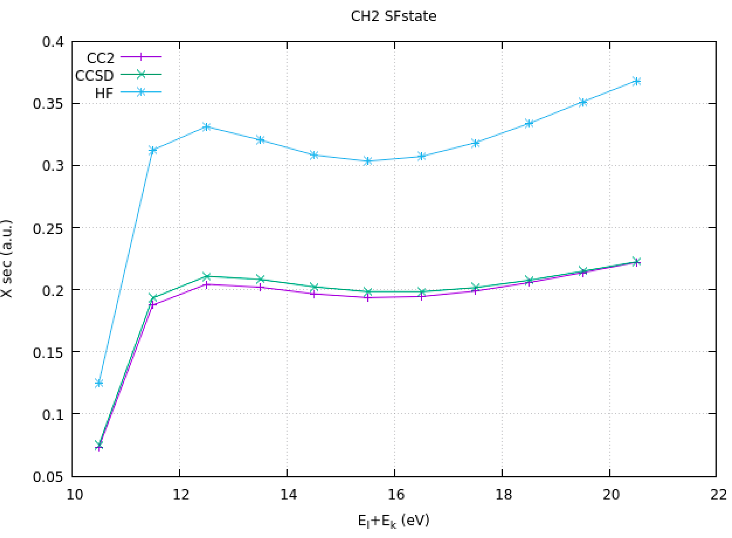
\includegraphics[width=0.6\textwidth]{chapters/appendix/image/Picture1.png}\\
\vfill
Formaldehyde, GS(HOMO)-IP, basis set: 6-31G*
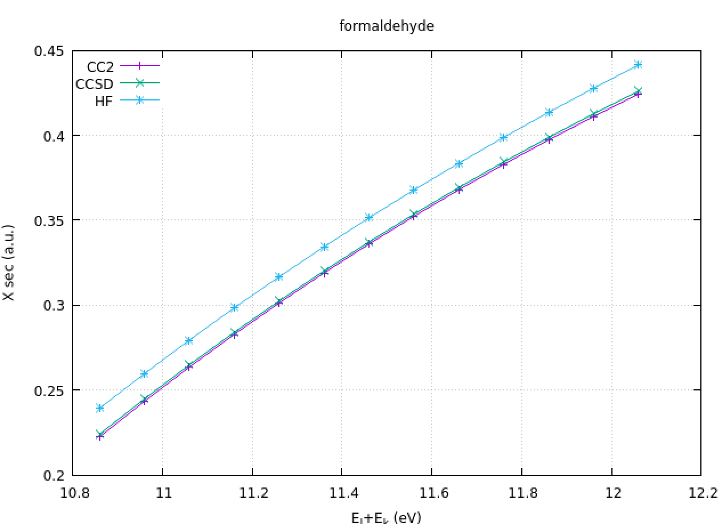
\includegraphics[width=0.6\textwidth]{chapters/appendix/image/Picture2.png}\\
\vfill
\clearpage

\vfill
\ch{OH-}, EE to IP [\ch{OH^{-*}} $\longrightarrow$ \ch{OH^{.}}], Basis set: 6-31G*
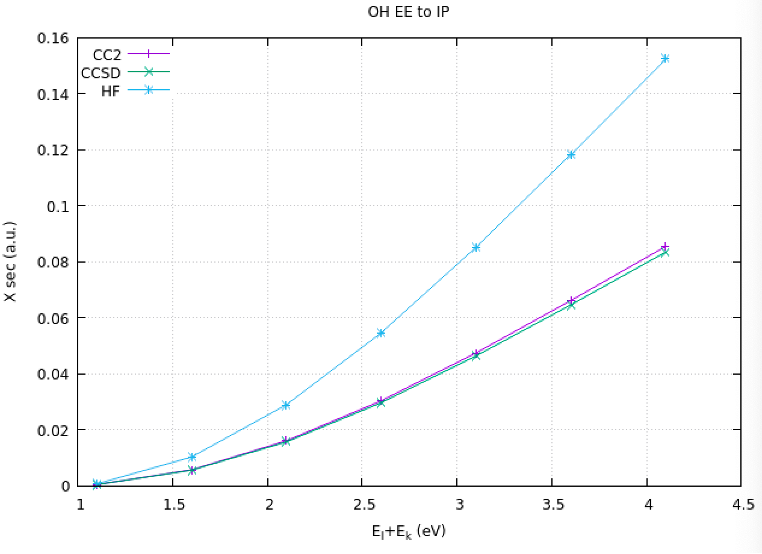
\includegraphics[width=0.6\textwidth]{chapters/appendix/image/OH-.png}\\
\vfill
\ch{NO}, EA($^2$B) -- GS [\ch{NO^*} $\longrightarrow$ \ch{NO+}], Basis set: aug-cc-pVTZ
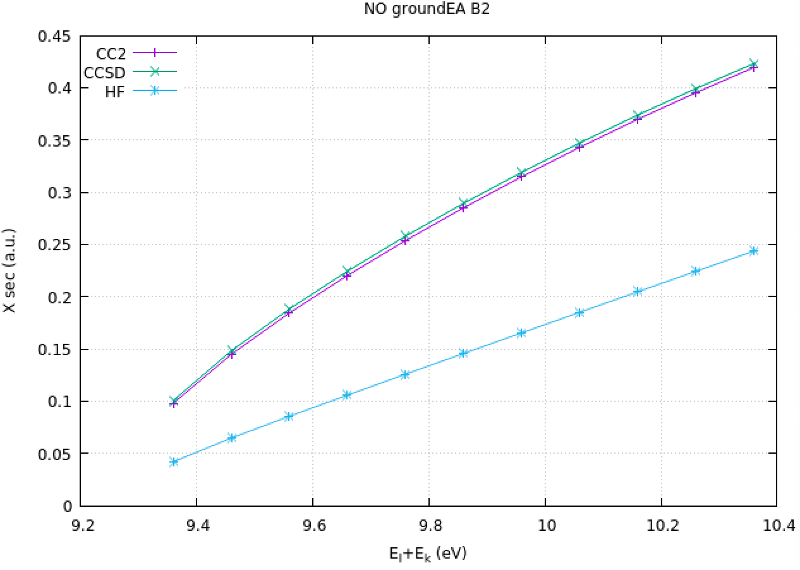
\includegraphics[width=0.6\textwidth]{chapters/appendix/image/NO.png}\\
\vfill
\ch{H2O}, GS(O 1s) -- IP [\ch{H2O} $\longrightarrow$ \ch{H2O^+}], Basis set: cc-pVTZ
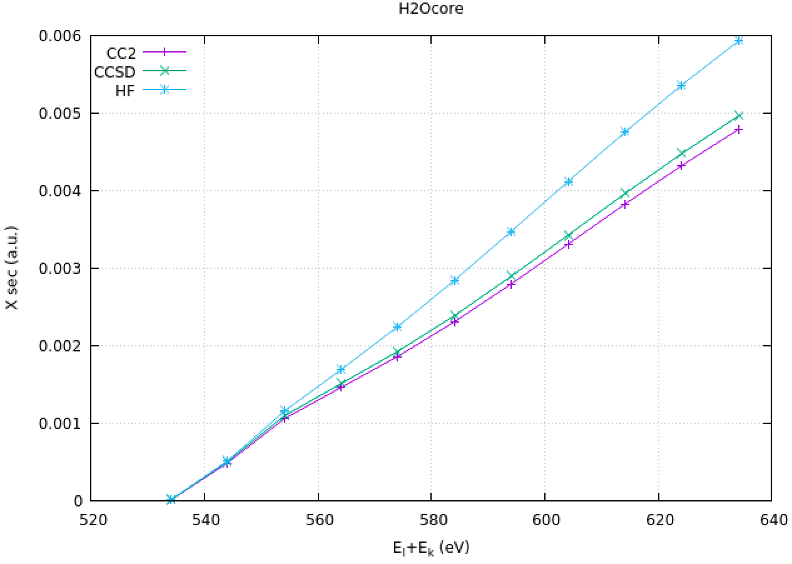
\includegraphics[width=0.6\textwidth]{chapters/appendix/image/H2O.png}\\
\vfill
\clearpage

\vfill
\ch{CO}, GS($^1$B or $^1$A) $\to$ IP [\ch{CO} $\longrightarrow$ \ch{CO^+}], Basis set: cc-pVDZ
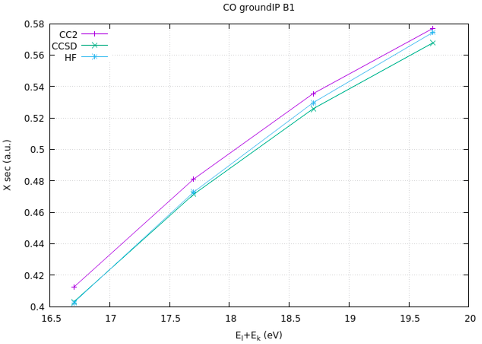
\includegraphics[width=0.5\textwidth]{chapters/appendix/image/CO1.png}
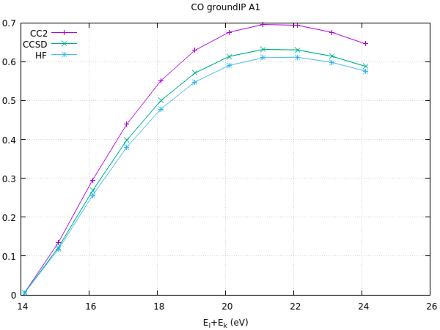
\includegraphics[width=0.49\textwidth]{chapters/appendix/image/CO2.png}\\
\vfill
\subsection*{Dipole-Bound Anions Photodetachment (aug-cc-pVTZ+6s3p)}
Acetone\\
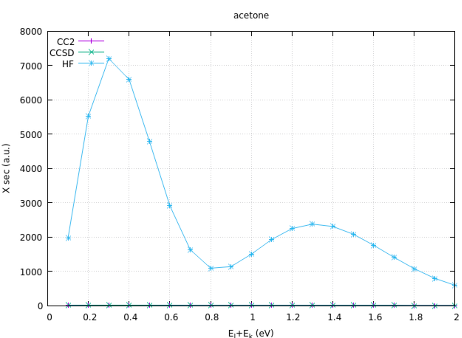
\includegraphics[width=0.49\textwidth]{chapters/appendix/image/Acetone1.png}
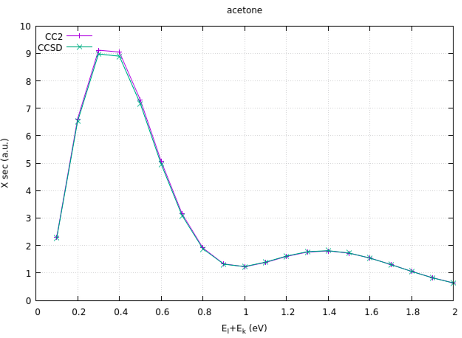
\includegraphics[width=0.49\textwidth]{chapters/appendix/image/Acetone2.png}\\
\vfill
Formamide\\
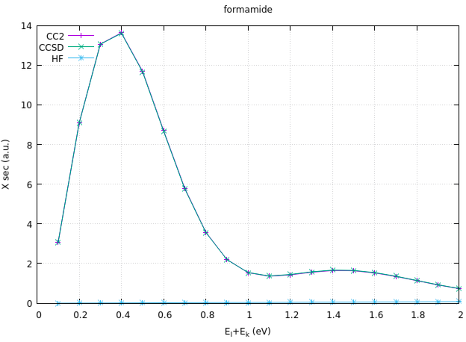
\includegraphics[width=0.48\textwidth]{chapters/appendix/image/Formamide1.png}
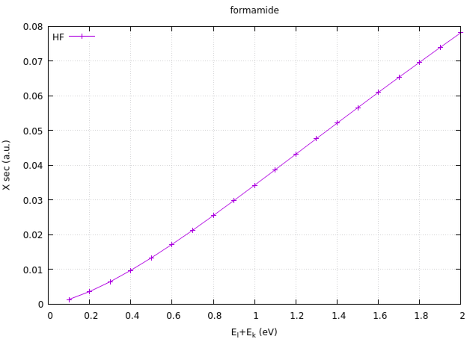
\includegraphics[width=0.48\textwidth]{chapters/appendix/image/Formamide2.png}\\
\vfill
\clearpage

\vfill
Nitrobenzene(DBS)\\
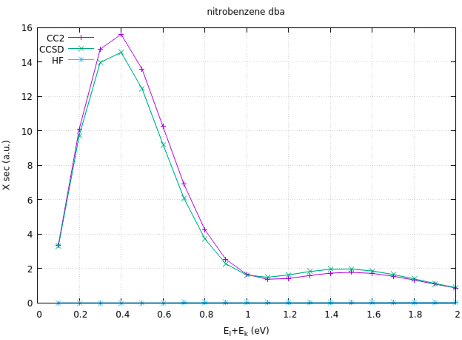
\includegraphics[width=0.49\textwidth]{chapters/appendix/image/Nitrobenzene1.png}
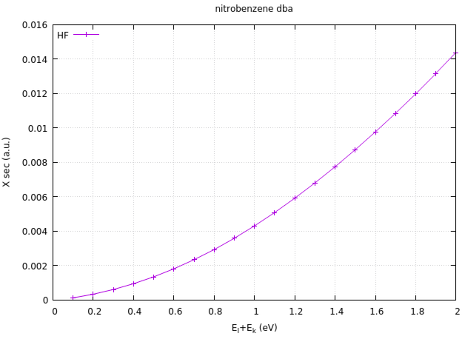
\includegraphics[width=0.49\textwidth]{chapters/appendix/image/Nitrobenzene2.png}\\
\vfill
\subsection*{Valence-Bound Anions Photodetachment (aug-cc-pVTZ)}
Benzoquinone\\
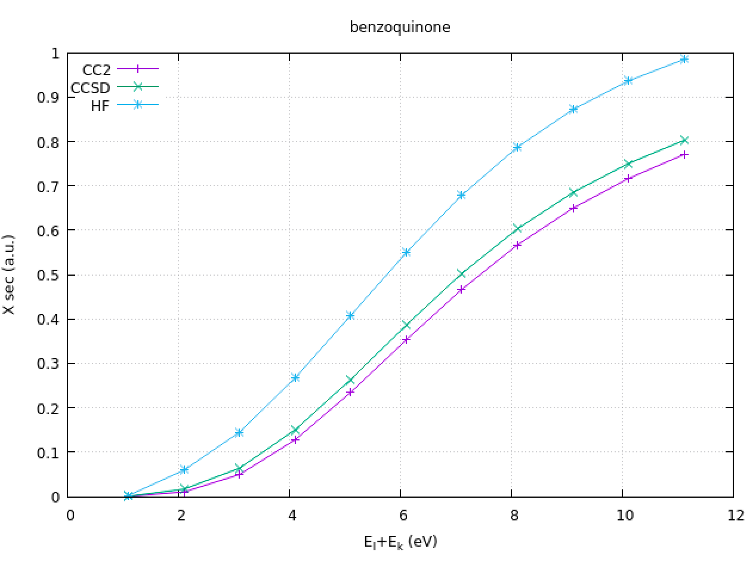
\includegraphics[width=0.6\textwidth]{chapters/appendix/image/benzoquinone.png}
\vfill
1,3-Dicyanobenzene\\
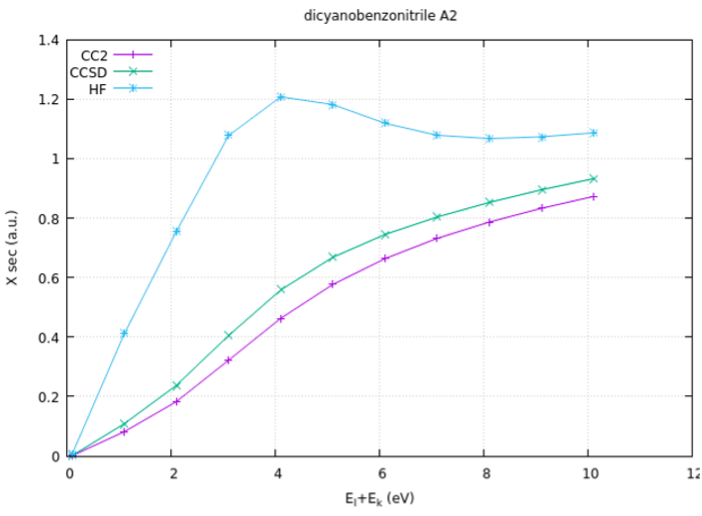
\includegraphics[width=0.49\textwidth]{chapters/appendix/image/diacyanobenzene1.png}
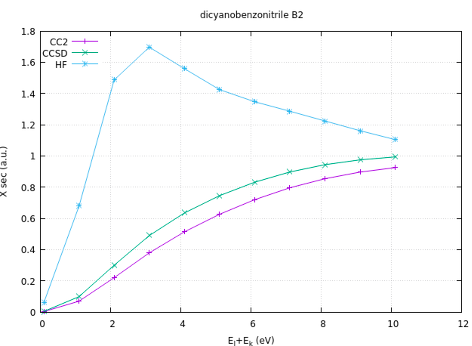
\includegraphics[width=0.49\textwidth]{chapters/appendix/image/diacyanobenzene2.png}\\
\vfill
\clearpage

\vfill
Maleic anhydride\\
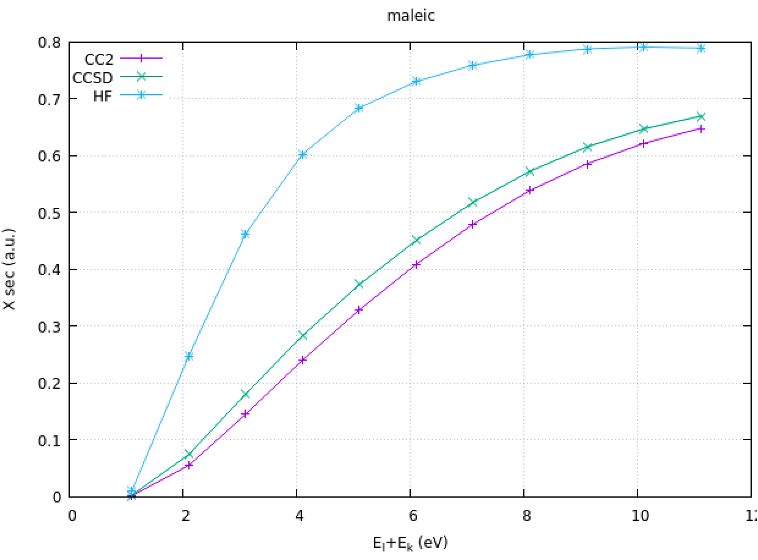
\includegraphics[width=0.6\textwidth]{chapters/appendix/image/maleic.png}
\vfill
Nitrobenzene(VBS)\\
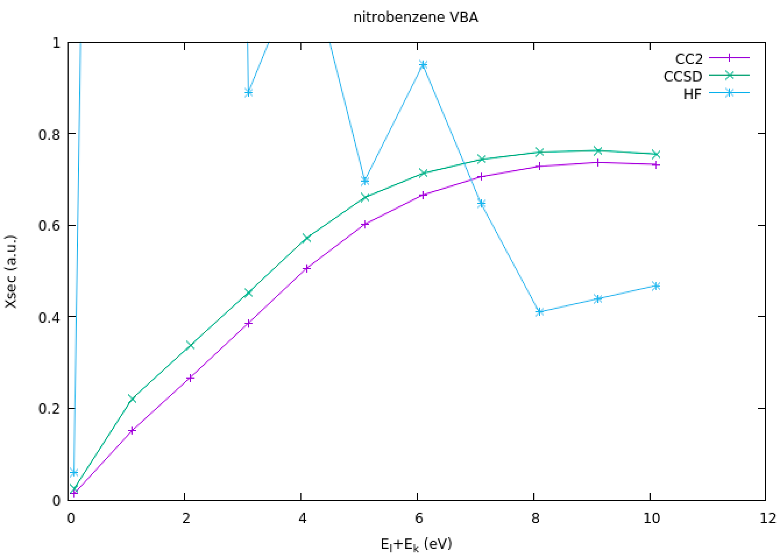
\includegraphics[width=0.6\textwidth]{chapters/appendix/image/nitrobenzeneVBA.png}\\
\vfill
Phenazine\\
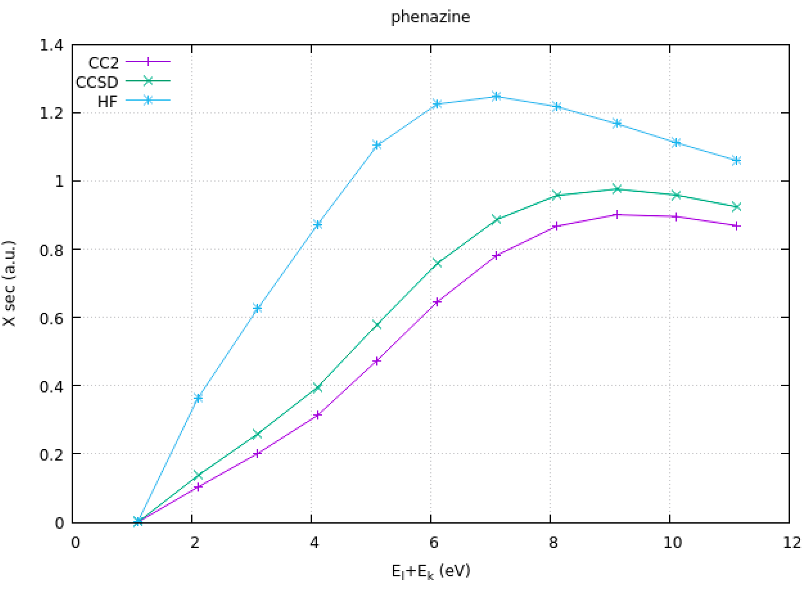
\includegraphics[width=0.6\textwidth]{chapters/appendix/image/phenazine.png}\\
\vfill




%%%%%%%%%%%%%%%%%%%%%%%%%%%%%%%%%%%%%%%%%%%%%%%%%%
% Keep the following \cleardoublepage at the end of this file, 
% otherwise \includeonly includes empty pages.
\cleardoublepage

% vim: tw=70 nocindent expandtab foldmethod=marker foldmarker={{{}{,}{}}}





\newpage
% ----------------------- Back cover ------------------------------
% Please fill in:
% - Department
% - Department's address
% - Telephone number and fax number
% -----------------------------------------------------------------
\thispagestyle{empty}
\sffamily
%
\begin{textblock}{191}(113,-11)
{\color{blueline}\rule{160pt}{5.5pt}}
\end{textblock}
%
\begin{textblock}{191}(168,-11)
{\color{blueline}\rule{5.5pt}{59pt}}
\end{textblock}
%
\begin{textblock}{183}(-24,-11)
\textblockcolour{}
\flushright
\fontsize{7}{7.5}\selectfont
\textbf{Quantum Chemistry and Physical Chemistry}\\
Celestijnenlaan 200F bus 2404\\
3001 LEUVEN, BELGI\"{E}\\
tel. + 32 16 37 21 98\\
jeremy.harvey@kuleuven.be\\
www.kuleuven.be\\
\end{textblock}
%
\begin{textblock}{191}(154,-7)
\textblockcolour{}
\includegraphics*[height=16.5truemm]{sedes}
\end{textblock}
%
\begin{textblock}{191}(-20,235)
{\color{bluetitle}\rule{544pt}{55pt}}
\end{textblock}
\end{document}
